\documentclass{article}


%%%%%%%%%%%% FORMATTING INCOMPATIBLE WITH UAI TEMPLATE %%%%%%%%%
%\usepackage[margin=1in]{geometry}
%\usepackage{parskip}

%\setlength{\skip\footins}{1cm}
%\setlength{\footnotesep}{0.4cm}


\usepackage{uai2020}
\usepackage[margin=1in]{geometry}
%\pagestyle{plain}

\usepackage{times}
	% Set the typeface to Times Roman
	% Not because it is better, but because it is UAI.
%joe3: it's a bad idea to use packages like this; 

%joe3: I don't have this package; it's probably a bad idea to use it	
\usepackage[backend=biber,
	style=authoryear,%alphabetic
%	citestyle=authoryear,
%	natbib=true,
	maxcitenames=1,
	url=true, 
	doi=true]{biblatex}
	

%joe3: all this should be unnecessary with a decent bibstyle
\DeclareCiteCommand{\parencite}[\mkbibparens]
	{\usebibmacro{prenote}}
	{\usebibmacro{citeindex}%
		\printtext[bibhyperref]{\usebibmacro{cite}}}
	{\multicitedelim}
	{\usebibmacro{postnote}}

        \usepackage[margin=1in]{geometry}
\usepackage{mathtools} %also loads amsmath
\usepackage{amssymb, bbm}

\usepackage[backend=biber,
	style=alphabetic,
	%	citestyle=authoryear,
	natbib=true,
	url=true, 
	doi=true]{biblatex}

%\usepackage{blkarray} % for matrices with labels
\usepackage{microtype}
\usepackage{relsize}
\usepackage{environ}% http://ctan.org/pkg/environ; for capturing body as a parameter for idxmats
\usepackage{tikz}
	\usetikzlibrary{positioning,fit,calc, decorations, arrows, shapes, shapes.geometric}
	\usetikzlibrary{cd}
	
	\pgfdeclaredecoration{arrows}{draw}{
		\state{draw}[width=\pgfdecoratedinputsegmentlength]{%
			\path [every arrow subpath/.try] \pgfextra{%
				\pgfpathmoveto{\pgfpointdecoratedinputsegmentfirst}%
				\pgfpathlineto{\pgfpointdecoratedinputsegmentlast}%
			};
	}}
	%%%%%%%%%%%%
	\tikzset{center base/.style={baseline={([yshift=-.8ex]current bounding box.center)}}}
	
	\tikzset{dpadded/.style={rounded corners=2, inner sep=0.9em, draw, outer sep=0.4em, fill=gray, fill opacity=0.08, text opacity=1}}
	\tikzset{active/.style={fill=blue, fill opacity=0.1}}
	\tikzset{square/.style={regular polygon,regular polygon sides=4, rounded corners = 0}}
	\tikzset{octagon/.style={regular polygon,regular polygon sides=8, rounded corners = 0}}
	
	
	\tikzset{alternative/.style args={#1|#2|#3}{name=#1, circle, fill, inner sep=1pt,label={[name={lab-#1},gray!30!black]#3:\scriptsize #2}} }
	
	
	\tikzset{bpt/.style args={#1|#2}{alternative={#1|#2|above}} }
	\tikzset{tpt/.style args={#1|#2}{alternative={#1|#2|below}} }
	\tikzset{lpt/.style args={#1|#2}{alternative={#1|#2|left}} }
	\tikzset{rpt/.style args={#1|#2}{alternative={#1|#2|right}} }
	\tikzset{pt/.style args={#1}{alternative={#1|#1|above}} }
	

	\tikzset{mpt/.style args={#1|#2}{name=#1, circle, fill, inner sep=1pt,label={[name={lab-#1},gray]\scriptsize #2}} }
	\tikzset{pt/.style args={#1}{name=#1, circle, fill, inner sep=1pt,label={[name={lab-#1},gray]\scriptsize #1}} }
	
		
		 %\foreach \x in {#1}{(\x) (lab-\x) } 
		 
	\tikzset{Dom/.style args={#1 (#2) around #3}{dpadded, name=#2, label={[name={lab-#2},align=center] #1}, fit={ #3 } }}
	\tikzset{bDom/.style args={#1 (#2) around #3}{dpadded, name=#2, label={[name={lab-#2},align=center]below:#1}, fit={ #3 } }}
	\tikzset{arr/.style={draw, ->, thick, shorten <=3pt, shorten >=3pt}}
	\tikzset{archain/.style args={#1}{arr, every arrow subpath/.style={draw,arr, #1}, decoration=arrows, decorate}}
	%\tikzset{every label/.append style={text=red, font=\scriptsize}}
	\tikzset{dpad/.style args={#1}{every matrix/.append style={nodes={dpadded, #1}}}}
	\tikzset{light pad/.style={outer sep=0.2em, inner sep=0.5em, draw=gray!50}}
	
	
	\newcommand\cmergearr[4]{
		\draw[arr,-] (#1) -- (#4) -- (#2);
		\draw[arr, shorten <=0] (#4) -- (#3);
	}
	\newcommand\mergearr[3]{
		\coordinate (center-#1#2#3) at (barycentric cs:#1=1,#2=1,#3=1.2);
		\cmergearr{#1}{#2}{#3}{center-#1#2#3}
	}

\NewEnviron{ctikzpicture}{\begin{center}\expandafter\begin{tikzpicture}\BODY\end{tikzpicture}\end{center}}
%\newenvironment{ctikzpicture}
%	{\begin{center}\begin{tikzpicture}}
%	{\end{tikzpicture}\end{center}}

\usepackage{color}
\definecolor{deepgreen}{rgb}{0,0.5,0}

\usepackage[colorlinks=true, citecolor=deepgreen]{hyperref}


\setlength{\skip\footins}{1cm}
\setlength{\footnotesep}{0.4cm}


\usepackage{stmaryrd}
\usepackage{trimclip}

\makeatletter
\DeclareRobustCommand{\shortto}{%
	\mathrel{\mathpalette\short@to\relax}%
}

\newcommand{\short@to}[2]{%
	\mkern2mu
	\clipbox{{.5\width} 0 0 0}{$\m@th#1\vphantom{+}{\shortrightarrow}$}%
}
\makeatother

\usepackage{parskip}
\usepackage{amsthm, thmtools}
\usepackage{
	nameref,%\nameref
	hyperref,%\autoref
	% n.b. \Autoref is defined by thmtools
	cleveref,% \cref
	% n.b. cleveref after! hyperref
}

\hypersetup{colorlinks=true, linkcolor=blue, urlcolor=magenta}

\begingroup
\makeatletter
\@for\theoremstyle:=definition,remark,plain\do{%
	\expandafter\g@addto@macro\csname th@\theoremstyle\endcsname{%
		\addtolength\thm@preskip\parskip
	}%
}
\endgroup
\makeatother

\theoremstyle{plain}
\newtheorem{theorem}{Theorem}[section]
\newtheorem{coro}{Corollary}[theorem]
\newtheorem{prop}[theorem]{Proposition}
\newtheorem{lemma}[theorem]{Lemma}
\newtheorem{fact}[theorem]{Fact}
\newtheorem{conj}[theorem]{Conjecture}

\theoremstyle{definition}
\newtheorem{defn}{Definition}[section]
\newtheorem*{defn*}{Definition}
\newtheorem{examplex}{Example}[section]
\newenvironment{example}
	{\pushQED{\qed}\renewcommand{\qedsymbol}{$\triangle$}\examplex}
	{\popQED\endexamplex\vspace{-1em}\rule{1cm}{0.7pt}\vspace{0.5em}}

\theoremstyle{remark}
\newtheorem*{remark}{Remark}

\usepackage{xstring}
\usepackage{enumitem}

\DeclarePairedDelimiterX{\infdivx}[2]{(}{)}{%
	#1\;\delimsize\|\;#2%
}
\newcommand{\kldiv}{D_\mathrm{KL}\infdivx}
%\DeclarePairedDelimiter{\norm}{\lVert}{\rVert}

%\newcommand\duplicat[1]{\gdef\mylist{}\foreach \x in {#1}{\xdef\mylist{\mylist (\x) (lab-\x) }}\mylist} %% this doesn't work :((
\newcommand\lab[1]{(#1)(lab-#1)}


\newcommand{\CI}{\mathrel{\perp\mspace{-10mu}\perp}}
\newcommand\E{{\mathbb E}}


\newcommand{\todo}[1]{{\color{red}\large\textbf{[}{\normalsize\texttt{todo:} \itshape#1}\textbf{]}}}
\newcommand{\note}[1]{{\color{blue}\large\textbf{[}{\normalsize\texttt{note:} \itshape#1}\textbf{]}}}

\newcommand\geqc{\succcurlyeq}
\newcommand\leqc{\preccurlyeq}
\newcommand\mat[1]{\mathbf #1}
\newcommand{\indi}[1]{\mathbbm{1}_{\left[\vphantom{\big[}#1 \vphantom{\big]}\right]}}
\newcommand\m[1]{\mathbf m_{\mathsf #1}}
\def\cpm#1(#2|#3){\mathbf #1 \left[ #2 \middle|#3\right]}


\newcommand\recall[1]{\expandarg\cref{#1}:\vspace{-1em} \begingroup\small\color{gray!80!black}\begin{quotation} \expandafter\csname #1\endcsname* \end{quotation}\endgroup }

%OMG THIS WORKS

\def\wrapwith#1[#2;#3]{
	\expandafter#2{\expandarg\StrBefore{#1}{,}}
	\expandarg\StrBehind{#1}{,}[\tmp] 
	\xdef\tmp{\expandafter\unexpanded\expandafter{\tmp}}
	#3
	\expandarg\IfSubStr{\tmp}{,}{\wrapwith{\tmp}[#2;{#3}]}{ \expandafter#2{\tmp} }
}
\def\hwrapcells#1[#2]{\wrapwith#1[#2;&]}
\def\vwrapcells#1[#2]{\wrapwith#1[#2;\\]}



\newsavebox{\idxmatsavebox}
\def\makeinvisibleidxstyle#1#2{\phantom{\hbox{#1#2}}}
\newenvironment{idxmatphant}[4][\footnotesize\color{gray}\text]{%
	\def\idxstyle{#1}
	\def\colitems{#3}
	\def\rowitems{#2}
	\def\phantitems{#4}
	\begin{lrbox}{\idxmatsavebox}$
	\begin{matrix}  \begin{matrix} \hwrapcells{\colitems}[\idxstyle]  \end{matrix} \\[0.1em]
		\left[ 
		\begin{matrix}
			\hwrapcells{\phantitems}[\expandafter\makeinvisibleidxstyle\idxstyle]  \\[-1em]
	}{
		\end{matrix}\right]		&\hspace{-0.5em}\begin{matrix*}[l] \vwrapcells{\rowitems}[\idxstyle] \end{matrix*}
	\end{matrix}
	$\end{lrbox}
	\raisebox{0.75em}{\usebox\idxmatsavebox}
%	\vspace{-0.5em}
}

\newenvironment{idxmat}[3][\footnotesize\color{gray}\text]
	{\begingroup\idxmatphant[#1]{#2}{#3}{#3}}
	{\endidxmatphant\endgroup}

\newenvironment{sqidxmat}[2][\footnotesize\color{gray}\text]
	{\begingroup\idxmat[#1]{#2}{#2}}
	{\endidxmat\endgroup}
	
	
%%%%%%%%%%%%
% better alignment for cases
\makeatletter
\renewenvironment{cases}[1][l]{\matrix@check\cases\env@cases{#1}}{\endarray\right.}
\def\env@cases#1{%
	\let\@ifnextchar\new@ifnextchar
	\left\lbrace\def\arraystretch{1.2}%
	\array{@{}#1@{\quad}l@{}}}
\makeatother
%        \usepackage[margin=1in]{geometry}
\usepackage{mathtools} %also loads amsmath
\usepackage{amssymb, bbm}

\usepackage[backend=biber,
	style=alphabetic,
	%	citestyle=authoryear,
	natbib=true,
	url=true, 
	doi=true]{biblatex}

%\usepackage{blkarray} % for matrices with labels
\usepackage{microtype}
\usepackage{relsize}
\usepackage{environ}% http://ctan.org/pkg/environ; for capturing body as a parameter for idxmats
\usepackage{tikz}
	\usetikzlibrary{positioning,fit,calc, decorations, arrows, shapes, shapes.geometric}
	\usetikzlibrary{cd}
	
	\pgfdeclaredecoration{arrows}{draw}{
		\state{draw}[width=\pgfdecoratedinputsegmentlength]{%
			\path [every arrow subpath/.try] \pgfextra{%
				\pgfpathmoveto{\pgfpointdecoratedinputsegmentfirst}%
				\pgfpathlineto{\pgfpointdecoratedinputsegmentlast}%
			};
	}}
	%%%%%%%%%%%%
	\tikzset{center base/.style={baseline={([yshift=-.8ex]current bounding box.center)}}}
	
	\tikzset{dpadded/.style={rounded corners=2, inner sep=0.9em, draw, outer sep=0.4em, fill=gray, fill opacity=0.08, text opacity=1}}
	\tikzset{active/.style={fill=blue, fill opacity=0.1}}
	\tikzset{square/.style={regular polygon,regular polygon sides=4, rounded corners = 0}}
	\tikzset{octagon/.style={regular polygon,regular polygon sides=8, rounded corners = 0}}
	
	
	\tikzset{alternative/.style args={#1|#2|#3}{name=#1, circle, fill, inner sep=1pt,label={[name={lab-#1},gray!30!black]#3:\scriptsize #2}} }
	
	
	\tikzset{bpt/.style args={#1|#2}{alternative={#1|#2|above}} }
	\tikzset{tpt/.style args={#1|#2}{alternative={#1|#2|below}} }
	\tikzset{lpt/.style args={#1|#2}{alternative={#1|#2|left}} }
	\tikzset{rpt/.style args={#1|#2}{alternative={#1|#2|right}} }
	\tikzset{pt/.style args={#1}{alternative={#1|#1|above}} }
	

	\tikzset{mpt/.style args={#1|#2}{name=#1, circle, fill, inner sep=1pt,label={[name={lab-#1},gray]\scriptsize #2}} }
	\tikzset{pt/.style args={#1}{name=#1, circle, fill, inner sep=1pt,label={[name={lab-#1},gray]\scriptsize #1}} }
	
		
		 %\foreach \x in {#1}{(\x) (lab-\x) } 
		 
	\tikzset{Dom/.style args={#1 (#2) around #3}{dpadded, name=#2, label={[name={lab-#2},align=center] #1}, fit={ #3 } }}
	\tikzset{bDom/.style args={#1 (#2) around #3}{dpadded, name=#2, label={[name={lab-#2},align=center]below:#1}, fit={ #3 } }}
	\tikzset{arr/.style={draw, ->, thick, shorten <=3pt, shorten >=3pt}}
	\tikzset{archain/.style args={#1}{arr, every arrow subpath/.style={draw,arr, #1}, decoration=arrows, decorate}}
	%\tikzset{every label/.append style={text=red, font=\scriptsize}}
	\tikzset{dpad/.style args={#1}{every matrix/.append style={nodes={dpadded, #1}}}}
	\tikzset{light pad/.style={outer sep=0.2em, inner sep=0.5em, draw=gray!50}}
	
	
	\newcommand\cmergearr[4]{
		\draw[arr,-] (#1) -- (#4) -- (#2);
		\draw[arr, shorten <=0] (#4) -- (#3);
	}
	\newcommand\mergearr[3]{
		\coordinate (center-#1#2#3) at (barycentric cs:#1=1,#2=1,#3=1.2);
		\cmergearr{#1}{#2}{#3}{center-#1#2#3}
	}

\NewEnviron{ctikzpicture}{\begin{center}\expandafter\begin{tikzpicture}\BODY\end{tikzpicture}\end{center}}
%\newenvironment{ctikzpicture}
%	{\begin{center}\begin{tikzpicture}}
%	{\end{tikzpicture}\end{center}}

\usepackage{color}
\definecolor{deepgreen}{rgb}{0,0.5,0}

\usepackage[colorlinks=true, citecolor=deepgreen]{hyperref}


\setlength{\skip\footins}{1cm}
\setlength{\footnotesep}{0.4cm}


\usepackage{stmaryrd}
\usepackage{trimclip}

\makeatletter
\DeclareRobustCommand{\shortto}{%
	\mathrel{\mathpalette\short@to\relax}%
}

\newcommand{\short@to}[2]{%
	\mkern2mu
	\clipbox{{.5\width} 0 0 0}{$\m@th#1\vphantom{+}{\shortrightarrow}$}%
}
\makeatother

\usepackage{parskip}
\usepackage{amsthm, thmtools}
\usepackage{
	nameref,%\nameref
	hyperref,%\autoref
	% n.b. \Autoref is defined by thmtools
	cleveref,% \cref
	% n.b. cleveref after! hyperref
}

\hypersetup{colorlinks=true, linkcolor=blue, urlcolor=magenta}

\begingroup
\makeatletter
\@for\theoremstyle:=definition,remark,plain\do{%
	\expandafter\g@addto@macro\csname th@\theoremstyle\endcsname{%
		\addtolength\thm@preskip\parskip
	}%
}
\endgroup
\makeatother

\theoremstyle{plain}
\newtheorem{theorem}{Theorem}[section]
\newtheorem{coro}{Corollary}[theorem]
\newtheorem{prop}[theorem]{Proposition}
\newtheorem{lemma}[theorem]{Lemma}
\newtheorem{fact}[theorem]{Fact}
\newtheorem{conj}[theorem]{Conjecture}

\theoremstyle{definition}
\newtheorem{defn}{Definition}[section]
\newtheorem*{defn*}{Definition}
\newtheorem{examplex}{Example}[section]
\newenvironment{example}
	{\pushQED{\qed}\renewcommand{\qedsymbol}{$\triangle$}\examplex}
	{\popQED\endexamplex\vspace{-1em}\rule{1cm}{0.7pt}\vspace{0.5em}}

\theoremstyle{remark}
\newtheorem*{remark}{Remark}

\usepackage{xstring}
\usepackage{enumitem}

\DeclarePairedDelimiterX{\infdivx}[2]{(}{)}{%
	#1\;\delimsize\|\;#2%
}
\newcommand{\kldiv}{D_\mathrm{KL}\infdivx}
%\DeclarePairedDelimiter{\norm}{\lVert}{\rVert}

%\newcommand\duplicat[1]{\gdef\mylist{}\foreach \x in {#1}{\xdef\mylist{\mylist (\x) (lab-\x) }}\mylist} %% this doesn't work :((
\newcommand\lab[1]{(#1)(lab-#1)}


\newcommand{\CI}{\mathrel{\perp\mspace{-10mu}\perp}}
\newcommand\E{{\mathbb E}}


\newcommand{\todo}[1]{{\color{red}\large\textbf{[}{\normalsize\texttt{todo:} \itshape#1}\textbf{]}}}
\newcommand{\note}[1]{{\color{blue}\large\textbf{[}{\normalsize\texttt{note:} \itshape#1}\textbf{]}}}

\newcommand\geqc{\succcurlyeq}
\newcommand\leqc{\preccurlyeq}
\newcommand\mat[1]{\mathbf #1}
\newcommand{\indi}[1]{\mathbbm{1}_{\left[\vphantom{\big[}#1 \vphantom{\big]}\right]}}
\newcommand\m[1]{\mathbf m_{\mathsf #1}}
\def\cpm#1(#2|#3){\mathbf #1 \left[ #2 \middle|#3\right]}


\newcommand\recall[1]{\expandarg\cref{#1}:\vspace{-1em} \begingroup\small\color{gray!80!black}\begin{quotation} \expandafter\csname #1\endcsname* \end{quotation}\endgroup }

%OMG THIS WORKS

\def\wrapwith#1[#2;#3]{
	\expandafter#2{\expandarg\StrBefore{#1}{,}}
	\expandarg\StrBehind{#1}{,}[\tmp] 
	\xdef\tmp{\expandafter\unexpanded\expandafter{\tmp}}
	#3
	\expandarg\IfSubStr{\tmp}{,}{\wrapwith{\tmp}[#2;{#3}]}{ \expandafter#2{\tmp} }
}
\def\hwrapcells#1[#2]{\wrapwith#1[#2;&]}
\def\vwrapcells#1[#2]{\wrapwith#1[#2;\\]}



\newsavebox{\idxmatsavebox}
\def\makeinvisibleidxstyle#1#2{\phantom{\hbox{#1#2}}}
\newenvironment{idxmatphant}[4][\footnotesize\color{gray}\text]{%
	\def\idxstyle{#1}
	\def\colitems{#3}
	\def\rowitems{#2}
	\def\phantitems{#4}
	\begin{lrbox}{\idxmatsavebox}$
	\begin{matrix}  \begin{matrix} \hwrapcells{\colitems}[\idxstyle]  \end{matrix} \\[0.1em]
		\left[ 
		\begin{matrix}
			\hwrapcells{\phantitems}[\expandafter\makeinvisibleidxstyle\idxstyle]  \\[-1em]
	}{
		\end{matrix}\right]		&\hspace{-0.5em}\begin{matrix*}[l] \vwrapcells{\rowitems}[\idxstyle] \end{matrix*}
	\end{matrix}
	$\end{lrbox}
	\raisebox{0.75em}{\usebox\idxmatsavebox}
%	\vspace{-0.5em}
}

\newenvironment{idxmat}[3][\footnotesize\color{gray}\text]
	{\begingroup\idxmatphant[#1]{#2}{#3}{#3}}
	{\endidxmatphant\endgroup}

\newenvironment{sqidxmat}[2][\footnotesize\color{gray}\text]
	{\begingroup\idxmat[#1]{#2}{#2}}
	{\endidxmat\endgroup}
	
	
%%%%%%%%%%%%
% better alignment for cases
\makeatletter
\renewenvironment{cases}[1][l]{\matrix@check\cases\env@cases{#1}}{\endarray\right.}
\def\env@cases#1{%
	\let\@ifnextchar\new@ifnextchar
	\left\lbrace\def\arraystretch{1.2}%
	\array{@{}#1@{\quad}l@{}}}
\makeatother
        
%\usepackage{subcaption}
\usepackage{comment}
%\usepackage{proof-at-the-end}


%%%% Version knobs %%%%%. 
%\includecomment{vfull}
\excludecomment{vfull}

%\includecomment{vcat}
\excludecomment{vcat}
\definecolor{notationcolor}{rgb}{0.9,0.9,.9} % purple

%\includecomment{vnotation}
\excludecomment{vnotation}

\newcommand{\notation}[2][]{#1}
\begin{vnotation}
	\renewcommand{\notation}[2][]{{\color{notationcolor} #2}}
\end{vnotation}

\newcommand{\commentout}[1]{\ignorespaces}
\newcommand{\vfullfootnote}[1]{}
\begin{vfull}
	\renewcommand{\vfullfootnote}[1]{\footnote{#1}}
\end{vfull}
%\excludecomment{nonintro}


%%%%%%% Commands to highlihght changes in the document.%%%%%%%%%%%%%%%%%%%%%
%\definecolor{note-fg}{rgb}{0.0,.4,0.2} % green
\definecolor{note-fg}{rgb}{.2,0,.4} % purple

%\newcommand\changed[1]{\colorbox{light gray}{\parbox{\linewidth}{#1}}}
\newcommand\changed[1]{{\color{note-fg} #1}}
\newcommand\changeon{\color{note-fg} }
\newcommand\changeoff{\color{black} }

\usetikzlibrary{external}
\tikzexternalize[prefix=tikz/]  % activate!

\AtBeginEnvironment{tikzcd}{\tikzexternaldisable} %... except careful of tikzcd...
\AtEndEnvironment{tikzcd}{\tikzexternalenable}

\newcommand\numberthis{\addtocounter{equation}{1}\tag{\theequation}}
%\crefname{section}{\S\!}{\S\!}

%joe3
%\usepackage[nointegrals]{ wasysym }

%\addbibresource{../refs.bib}
%\addbibresource{../uncertainty.bib}
%\addbibresource{../maths.bib}
%\addbibresource{graphical-models.bib}

% symbols for genders, hour glass.
%\newcommand{\mfem}{\mathclap\female\male}
%\newsavebox{\hourglassbox}
%\savebox{\hourglassbox}{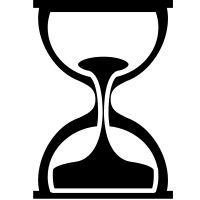
\includegraphics[height=.8em]{hourglass.png}}
%\newcommand\hourglass{\usebox{\hourglassbox}}

%%%%%%%%%%%%%%%% SHORTCUTS FOR COMMONLY USED THINGS %%%%%%%%%%%%%%

\newcommand\Set{\textbf{Set}}
\newcommand\FinSet{\textbf{FinSet}}
\newcommand\MeasSet{\textbf{MeasSet}}

% Semantics
%joe3: using lower case, to match text
%\newcommand\SD{_{\text{SD}}}
\newcommand\SD{_{\text{sd}}}
%\newcommand\Weighted{_{\text{WD}}
		
%\newcommand\MaxEnt{{\substack{\mathbf{Max}\\\mathbf{Ent}}}}
\newcommand\MaxEnt{_{\mathbf H}}


\newcommand{\none}{\varobslash}
\def\sheq{\!=\!}
\newcommand{\lowrightarrow}[1]{\mathrel{\raisebox{-2pt}{$\xrightarrow{#1}$}}}
\DeclareMathOperator\dcap{\mathop{\dot\cap}}
\newcommand{\doubleheadrightarrow}{%
	\rightarrow\mathrel{\mspace{-15mu}}\rightarrow}


%\def\bmu[#1|#2]{\boldsymbol\mu\boldsymbol{[} #1 \boldsymbol{|} #2 \boldsymbol{]}}

\newcommand\bb[1]{\mathbbm{#1}}

\newcommand{\bmu}{\boldsymbol{\mu}}
\newcommand{\V}{\mathcal V}
\newcommand{\N}{\mathcal N}
\newcommand{\Ed}{\mathcal E}
\newcommand{\sfM}{\mathsf M}

%%%%%%%%%%%%%%%%%%%%%%%%%%%%%%%%%%%%%%%%%%%%%%%%%%%%%%%%%%%%%%%%%%


%%% What do I even call them anyway?
\newcommand{\ModelName}{Probabilistic Dependency Graph}
\newcommand{\modelname}{probabilistic dependency graph}
\newcommand{\modelnamehyper}{probabilistic dependency hypergraph}
\newcommand{\modelnames}{\modelname s}
\newcommand{\MN}{PDG}
\newcommand{\MNH}{PDH}
\newcommand{\MNs}{\MN s}

\numberwithin{equation}{section}

\title{\ModelName s}

\author{} % LEAVE BLANK FOR ORIGINAL SUBMISSION.

%% UAI  reviewing is double-blind.
%
%% The author names and affiliations should appear only in the accepted paper.
%%
%\author{
%	{\bf Oliver E. Richardson%\thanks{Footnote for author to give an alternate address.}
%		}\\
%%	Computer Science Dept. \\
%	Cornell University\\
%	Address\\
%\And
%	{\bf Joseph Y. Halpern}  \\
%	Cornell University      \\
%	Address \\
%}
%


\begin{document}
	\maketitle
	
	\begin{abstract}
		We introduce a new type of graphical model, \emph{\ModelName s} (\MNs).  
		They can capture inconsistent beliefs in a natural way and are, in a precise sense, more modular than standard
		approaches such as Bayesian networks (BNs), 
		in that they make it easier for	a modeler to incorporate new information 
		%oli1: this feels like the wrong sense: they make it
		%easier to re-structure information! 
		\commentout{without having to restructure
			the representation of current information.}
		%joe2: Sorry, Oliver, I don't like this. I don't know what it means to
		%``finalize'' a distribution.   I doubt anyone else will either.  I
		%also don't see why it's true, under any reasonable interpretation.  
		and restructure the representation, without having to
		finalize a distribution. 
		%joe1*: this is a point you should trumpet loudly
		%oli1: untangle the sentence
		\commentout{As we show, when viewed as a \MN, a BN $G$
			represents many}
		%joe2: the names don't help; changing the name doesn't convert it from
		%being a PDG to a BN                
		%		As we show, a BN $G$, when viewed as a \MN\ $\sfM$,
		As we show, a BN, when viewed as a \MN,
		may represent many 
		%joe2
		%	 distributions, but we can recover the one given by the
		distributions, but we can recover the distribution given by the
		semantics of BNs as 
		the one that maximizes entropy among all the distributions consistent
		with $\sfM$.  
		%joe1: we may want to say a bit more, or beef up this sentence
		We show by example how \MNs\ are a natural modeling tool.
		%joe2: it's not clear that we need to say more in the abstract,
		%although I don't have strong feelings about it
		\todo{add more of the results we agree go in the final version}
	\end{abstract}

%	\tableofcontents

	\section{INTRODUCTION}

	\commentout{We introduce the \ModelName\ (\MN), a directed graphical model for specifying local beliefs. They are strictly more expressive and modular than existing directed graphical models, and in particular this allows them represent inconsistent belief states.
	
	
	To be clear, inconsistencies are bad. Still, constantly examining every possible interaction between beliefs is taxing and restrictive, making them difficult to avoid: reasonable people are often simultaneously unaware of any inconsistencies in their beliefs, and yet still think it probable that they are not entirely consistent.%
%oli1: what do you think of the point in this footnote? Do you think it's worth bringing up somewhere? 
%joe2: I don't think it adds much, and I think there are many other
%reasons that arguments exist.
		\footnote{In some sense, this is the reason arguments exist: it is possible to get a person to agree to premises and reject a conclusion, revealing inconsistency---inconsistency which can then be used to change someone else's mental state. }		
	Most graphical models eliminate the possibility of inconsistency by fiat, 
	making them poorly suited to representing inconsistent belief states.
	While we do not endorse inconsistency, we nonetheless think it important to represent: in addition to modeling an overwhelmingly common feature of humans, the possibility of inconsistency 
	allows our model (called a \modelname\ or \MN)
	to portray intermediate stages of belief updating (\Cref{sec:belief-update}), 
	provides a rationale for providing multiple justifications 
	(corroborating evidence means more in the presence of possible conflict; see \Cref{ex:corrob}),
	and	recasts standard algorithms such as belief propagation and conditioning on evidence as resolutions of inconsistency (\Cref{sec:algorithms}). }

%joe1*: the first paragraph is where you grab the reader.  You need to
%tell a story.  This is not telling our story.  I've rewritten the
%whole beginning
In this paper we introduce yet another graphical for modeling beliefs,
\emph{Probabilistic Dependency Graphs} (PDGs).  
There are already many such models in the literature, including 
%joe1: we probably should add some standard references to these
%approaches.  
%oli1: I've added some, but perhaps these are not ideal
%joe2: perhaps we can ust say ``See \cite{KF09} [that's the
%Koller-Friedman ref in joe.bib] for an introduction to and discussion
%of these representations.
%oli2: I'm ok with this, except this was before directed factor graphs.
%oli2: edited.
Bayesian networks (BNs), factor graphs \parencite{koller2009probabilistic},
unifications of 
these such as directed factor graphs \parencite{frey2012extending},
and conditional versions of all three. 
Why does the world need one more?

Our original motivation for introducing PDGs was to be able to capture
inconsistency.  
While being inconsistent is clearly not a good thing,
we wanted to be able to model the process of resolving inconsistency;
to do so, we had to be able to model the inconsistency itself.  
But our approach to modeling inconsistency has many other advantages.
%oli1: I've taken most of your suggestions and merged some of my old points back in
% that I think deserve a spot in the story.
%joe2: I'm afraid that we're not converging.  As you'll see, I've
%undone your changes.  I try to explain why.
% that I think deserve a spot in the story.
%joe3: removed paragraph break

In particular, as we shall see, \MN s are significantly more modular
than other approaches.
%joe3*: I don't know how we modify the graph without changing it's
%informational content.  That doesn't make sense to me.  I also don't
%now what it means to add information ``efficiently''
%We can efficiently both add new information to a graph
%without changing the existing structure, 
%and also modify the graph without changing its informational content.
% Though we may incur inconsistency by doing so, relaxing this
% coupling makes it easier to talk about representational learning.
We can easily add new information to a graph
without changing the existing structure. 
%joe2: Cut; I don't understand what it means to ``consolidate
%computational costs'', and we don't discuss this issue. 
%oli2: Rather than paying the update cost for every observation and
%thought, you can just incorporate observations and think about them
%later. This seems very congruous with the story, and in particular
%with the ``you may not want to resolve conflicts right away'' bit,
%partly because it's expensive. I don't know the bit I wrote
%specifically about this is still in the document or not. 
%joe2: I also don't know what it would mean for a representation to be
%more dramatic. 
%This is a case of ``show, don't tell''.  Let the examples do the talking.
%oli2: I agree and I should probably get some more examples. Still I
%wanted this paragraph to go somewhere: it seems to me the reason it's
%beneficial to the things you're keeping track of, and the processing
%you need to make sense of it, is because you can do weirder graph
%transformations and resolve all of the inconsistency at once, rather
%than ensuring things are up-to-date at all times. 
%oli2*: Analogy: constantly making sure the document has the right
%formatting. Ultimately the formatting may help but making sure it's
%corretly formatted after every character you type is `taxing and
%restrictive'. Fixing your habits allows you to make bigger
%modifications to the document, and consolidate the cost of fixing the
%formatting.
%joe3: maybe so, but if you're going to claim this, you have to give
%examples.   You can't just make the claims
%	As a result, we can make more dramatic transformations of
%        representation, and consolidate the computational costs of
%        resolving them. 
%
%
%joe2: Oliver, instead of spraying the reader with a lot of
%unexplained bullets, you need to go over these points carefully
%later, and explain them.  I assume that by ``theoretical backing''
%you mean semantics.
%oli2: I am really referring to how nicely the energy and composition
%bits work out, compared to some other graphical models which I view
%as hackier: by thinking of the tables as being in the edges, lots
%things seem to magically fall into place. Most of these things I know
%I won't be able to explain in this space, but I want to get to at
%least the energy and composition. I know I need to support this later
%if I want it in the intro. If I can't get to convincing examples by
%the end I agree we need to cut it.
%joe3: not only do you have to support it.  You shouldn't bring it up
%until you've illustrated it.
%joe2: The semantics is discussed later.  If you mean something else, you
%have to make it clear.  I don't know what it means to ``promise
%deeper parallels''.  Let the examples show how PDGS are a natural
%etension, rather than saying it. 
%oli2: While examples are definitely be better than hand waving,
%though this would not be the place for them. We are advertising the
%story at a high level here; I'm trying to mark this as something I
%want in the story, in the same way that we're trying to advertise
%modulairty without examples at this point.
%joe3: You don't ``advertise'' modularity just by saying you have it.
%Sometimes you can get away with saying ``As we shall show, ...'', but
%you want to minimize that
%joe2: We really don't want to talk about
%type thoery here, nor do we want to make mysterious claims about
%locality.  That's not what an introduction is for.  I cut all this.
%	Furthermore, the theoretical backing is clean, promising
%        deeper parallels to other fields.  
%	\MNs\ themselves are natural extensions of BNs, and the nature
%of this extension complements both the information theoretic
%foundations of graphical models (\Cref{sec:thermo}) and the type
%theory we gesture towards. 
%	The modifications we make also bring graphical models in line
%        with other notions of locality in mathematics,  
%joe1: If you're going to bring these up, you would have to explain
%the connection.  We do not want to do that here (maybe somewhere much
%later in the full paper), so we shouldn't mention it here.  If you
%mention it, you need to add references.
%oli1: why should it here? We haven't fully explained anything yet. I mention it again when I the union precisely.
%oli1: I've now added one possible reference but I'm not really leaning on it. There are a bunch of 
% related constructions and I call out manifolds because everyone has heard of them, but if you can read the reference
% you probably also know this happens all over the place. You might not have realized that this was similar to the union
% construction if I don't mention it though.
%joe2: NO! we don't want to bring this up in the second paragraph of
%the introduction, before you've given the reader some
%intuitions. Maybe you can hint at some of this stuff in the
%discussion section at the end.  But it definitely shouldn't go here
%oli2: Ok. I'm now on the same page about cutting this, but I'm still
%confused about how this is different from the sentence advertising
%and then explaining modularity.
%joe3: in that case, you explained it right away.  Here you don't
%	such as manifolds \parencite[e.g.,][p.12]{atlases}, in which
%        multiple restricted pictures can be glued together to form
%        something with global structure. 
%
%	We start by giving some examples that motivate PDGs and display some of their advantages over Bayesian Networks in particular.
	We start with some examples to motivate \MNs\ and display some
%joe3: it's OK to recap some advantages at the ed, but many of the
%ones on your list are ones we won't get to in the paper.
%        of these advantages; those looking for a more comprehensive
        %        list can skip to \Cref{sec:list-of-benefits}.
of these advantages.
%	We use the rest of the section to give some of examples focusing on the benefits of this improved modularity, motivate the design of agents that might , and highlight the failure of Bayesian Networks to capture what we have in mind (we compare to other graphical models in \Cref{sec:other-graphical-models,sec:many-relations-graphical-models}). \MNs\ have other desirable features as well; for a complete list, see \Cref{sec:list-of-benefits}.
	
	\begin{example}\label{ex:guns-and-floomps}
		You arrive in a foreign country known for having very clear laws. From prior reading, you ascribe probability 0.95 to owning guns being against the law. Upon arrival, you end up talking to some teenagers who use the local slang, 
		after which you believe that with probility .1, the law prohibits floomps. 
		
		The obvious way to represent this as a BN involves two binary random variables, $F$ (taking values $\{f, \overline f\}$), indicating the legality of floomps, and $G$ (taking values $g, \overline g$) indicating the legality of guns. 
		The semantics of a Bayes Net offer us two choices:
		we either assume that $F$ and $G$ are independent and give
%oli1: `priors' seems wrong, I want to say marginals.
%joe2: people talk about them as priors.  The key point is that they're unconditional
%oli2: I'm also ok with priors, which is shorter. I also thought
%marginals were almost always unconditional, 
% 	which is why `marginal constraint graph' felt like the wrong name for PDGs.
%		priors for $F$ and $G$, or we choose a
%joe3: actually, on further though, marginal imply that there's a
%probability on a big space which is being marginalized.  While that's
%true, that's not how it's presented.  I just went with the sipmler
%``probability'' 
%they're unconditional (unconditional) marginals of $F$ and $G$, or we choose a
		(unconditional) probability of $F$ and $G$, or we choose a
		direction of dependency,
%joe3: incorporate one of the two what?  what does ``incorporate''
%mean here?
%                in which case we can only incorporate one of the two,
                and must give a conditional probability table.           
		As there is no reason to believe that either variable depends on the
		other, the natural choice is to assume independence, giving us the
		following BN:
		
		
		\begin{center}
			\scalebox{0.9}{
			\begin{tikzpicture}[scale=0.8,ampersand replacement=\&]
	
				\node[dpadded, circle] (floomp) at (-1.2,0) {$F$};
				\node[dpadded, circle] (gun) at (1.2,0) {$G$};
	
				\matrix [table with head, column 1/.style={leftrule},
					 column 2/.style={rightrule}, row 2/.style={bottomrule}] at (-3.5,0)	{
					\vphantom{$\overline f$} $f$ \& $\overline f$\\
					.9 \& .1\\
				};
				\matrix [table with head, column 1/.style={leftrule},
					 column 2/.style={rightrule}, row 2/.style={bottomrule}] at(3.5,0)	{
					 \vphantom{$\overline g$}$g$ \& $\overline g$\\
					 .05 \& .95\\
				};
			\end{tikzpicture}
			}
		\end{center}
		
		Now suppose that you later discover that ``floomp'' is likely to be another word for gun, and come to believe that if floomps are legal (resp., illegal), then there's a 92\% chance guns are as well.
		Let $T$ be the conditional probability table (cpt) that describes this belief.
		A first reaction might be to simply incorporate this conditional information by
		adding $F$ as a parent of $G$, and then associating the cpt $T$ with $G$.
		But then what should we do with the original probability we had
		for $G$?  Should we just discard it?
			% which amounts to throwing out our old prior distribution on $G$; 
			% another instinct might be to perform a Bayesian update, but this new information is conditional and probabilistic, not an event.
		It is easy to check that there is no probability distribution that is
		consistent with the two original priors on $F$ and $G$ and also the cpt
		$T$, so if we are to represent our information with a BN, we must
		resolve the inconsistency.  
%		In fact, $E$ conflicts with the other two tables, in the sense that there is no joint distribution on $\{F, G\}$ such that all three tables are accurate. 
%		Therefore, there is no Bayes Net that contains all three pieces of information exactly: one has to resolve the inconsistency first.
			
		%There are three different dimensions along which this could be resolved: rejecting either prior belief, or $E$; in general any mixture would do. 
                %joe3: removed paragraph break, and discussion of
                %``your interests'', which are largel irrelevant
%		
%However, it may not be in your best interest to sort this out right away.
However, it may be better not to sort this out right away.
		How to resolve it may be clearer if you can get confirmation
		that guns are indeed floomps, or read the laws more carefully.


		By way of contrast, consider the corresponding \MN. In a \MN, the cpts
		are attached to edges, rather than nodes of the graph.  
		The cpt associated with an edge $e$ is a matrix
		$\mat e$, where the element $\mat e_{a,b}$ at row $a$ and column $b$
		is the conditional probability $\Pr(B \!\!=\!\!b \mid A \!\!=\!\! a)$.  
%		We will represent the cpt for a edge $L \!\colon\! A\!\to\! B$ as matrices $\mat L$, whose element $\mat L_{a,b}$ at row $a$, column $b$ is the conditional probability $\Pr(B \!\!=\!\!b \mid A \!\!=\!\! a)$. 		
		In order to represent unconditional probabilities% (among other things; see section \ref{sec:algebra})
		, we introduce a \emph{unit variable} $\mathsf 1$ %, or `$\mathrm{true}$',
		which takes on only one possible value,	which we denote $\star$.
%joe3: removed paragraph break		
%		
		Thus, we have the \MN\ depicted in \Cref{fig:gun-floomp-diagram}, where the edges from $\mathsf 1$ to $F$ and $G$ are
		associated with the unconditional probabilities of $F$ and
		$G$, and the edge from $F$ to $G$ is associated with
		the cpt $T$.
		\begin{figure}[h]
			\centering
			\scalebox{0.9}{
			\begin{tikzpicture}
				\node[dpadded] (true)  at (0,1.7) {$\mathsf 1$};
				\node[dpadded] (floomp) at (-1.5,0) {$F$};
				\node[dpadded] (gun) at (1.5,0) {$G$};			
				
				\draw[arr] (true) -- coordinate(A) (floomp);
				\draw[arr] (true) -- coordinate(B) (gun);
	
				\node[above left=0.5em of A] {
					\begin{idxmat}{$\star$}{$f$, $\overline f$}
						.90 & .10 \\
					\end{idxmat}
				};
				\node[above right=0.5em of B] {
					\begin{idxmat}{$\star$}{$g$, $\overline g$}
						.05 & .95 \\
					\end{idxmat}
				};
	
				\definecolor{heldout}{rgb}{0.7,0.7,1}	
				\draw[heldout, dashed, arr] (floomp) -- coordinate(C) (gun);
				\node[below=1em of C] {
					\color{heldout}
					T =\begin{idxmat}[\footnotesize\color{heldout}\text]{$f$,$\overline f$}{$g$, $\overline g$}
						0.92 & 0.08 \\ 0.08 & 0.92 \\
					\end{idxmat}
				};
			\end{tikzpicture}
			}
			\caption{An inconsistent \MN, requiring resolution}
			\label{fig:gun-floomp-diagram}
		\end{figure}
                %joe3
%		
		The original state of knowledge consists of all three
                nodes and the two black edges  e  $\mathsf 1$. This is
%joe3
%                like our Bayes Net from before, except we no longer
   like Bayes Net that we considered abovefrom before, except we no longer
                assume that $F$ and $G$ are independent; 
	%oli2: I implemented your change but personally I like "assume
        %... to be indep" much more than "assume that ... are indep" 
		we merely record the constraints imposed by the given probabilities.
	
		\begin{vfull}
		\note{\emph{(This is from our discussion but parts of it seem out of the way so I haven't integrated it yet. It probably needs to be moved.)}
			
			A proponent of Bayes Nets might argue: sure, we've assumed independence, but that was on purpose! We get a lot of mileage out of independence assumptions, and they're expensive to encode explicitly.
			
			Sure enough, if we wanted to explicitly encode such an independence assumption without making it part of the the background machinery for all diagrams, one would need to either give a edge $F \to G$ (or vice versa) whose table has an identical distribution over $G$ every row, or specify the joint distribution directly, as below...
			
			\centerline{\scalebox{0.8}{
			\begin{tikzpicture}
				\node[dpadded] (true)  at (0,1.7) {$\mathsf 1$};
				\node[dpadded] (floomp) at (-1.5,0) {$F$};
				\node[dpadded] (gun) at (1.5,0) {$G$};
				\unmergearr{true}{floomp}{gun}
			\end{tikzpicture}
			}}
		
			These tactics save no representational space, making them useless for compressing distributions, may not even then may not display the dependency structure we had in mind. 
			
			Fortunately, the multiple semantics of \MNs\ allow us to eat our cake and have it too: by recording only the constraints, we avoid leaning too hard on independence assumptions, but can still reap the benefits through maximum-entropy semantics: the maximum entropy distribution associated with the constraints is the one prescribed by the Bayesian Network.
		}
		\end{vfull}
	
		The key point here is that we can incorporate the new information into
		our original representation (the graph in \Cref{fig:gun-floomp-diagram}
		without the edge from $F$ to $G$) simply  by adding the edge from $F$
		to $G$ and the associated cpt.  Doing so does not change the meaning
		of the original edges.  The added modularity lets us simply include
		information, and resolve inconsistencies later. Unlike a Bayesian
		update, the operation is even reversible: all we need to do recover
		our original belief state is delete the new edge, effectively making
		it possible to mull over and then reject an observation.
	\end{example}

	It may seem that, while our approach has advantages, we have lost a
	key benefit of BNs: the ability to exploit (conditional)
	independencies, which, as \textcite{pearl2014probabilistic} has argued
	forcefully, are omnipresent.  As we shall see, this is not the case.  
  %joe3: added
We can recover the (probability distribution represented by the)
Bayes Net from the set of distribution consistent the PDG.
We returnto this point below; for now, we show that 
	%joe1: 	shortened.  Please don't talk about coloring out of the blue.
	%oli: I've modified but not used your replacement paragaph.
%joe2: we should be consistent about single quote vs. double quotes.
%You later use double quotes.  Moving up a level, whats the difference
%between ``over-constrained'' and inconsistent?  Why distinguish
%them.  
%oli2: see my new note after definition 3.2
%joe3: I'm afraid that didn't help at all.  See below.
%joe2: Moreover, it's notthe ability to represent
%inconsistency/over-constrained states that's useful when there's no
%inconsistency, but the modularity.  Reverting back.  
%oli2: It's both. The over-constrainedness is helpful for slightly different
% reasons though: like I wrote earlier in the intro at some point,
% there's a benefit in corroborating evidence, and agreement is more meaningful
% if there could have been non-agreement.
%joe3: It might be OK to say this if you then gave an example.  
%In general, 
%	The ability to represent these ``over-constrained'' states of
%        belief, in which inconsistency is possible, can also be
%joe2
%   valuable even when there isn't any.
%joe3
%The modularity of PDGs is useful even when there is no
%inconsistency, as the following example shows. 
the modularity of PDGs can be useful even when there is no
inconsistency.
%joe2: Cut; what do ``observed nodes'' have to do with
%under-constrained beliefs.  What makes a conditional belief
%underconstrained?   There's a simple clean story here, and you're
%bringing in all bunch of issues and spraying the reader with them,
%without explaining them in context. I cut this again.
%	Unlike standard conditional models, which require a special
%        selection of `observed' nodes, \MNs\ also cleanly represent
%        `under-constrained' beliefs, such as conditional ones,   without
%              selection of `observed' nodes, \MNs\ also cleanly represent
%        `under-constrained' beliefs, such as conditional ones, without
%        modification. 
%	Our next example illustrates both, and highlights one more way
%in which BNs fail to be as modular as we might hope. 
%oli1: what we lose in this shortening:
% 1. beginning to introduce `over-constrained' and `under-constrained'
% terminology. I think this is useful for understanding why the set
% semantics are not enough, and drawing a parallel to
%joe2: we've alrady introduced over-constrainedness.  You're not
%introducing under-constrainedness; you're just using a word without
%explaining it.
% 2. no segue into conditional models, or acknowledgement that they
% are the standard solution to under-constrainedness
%joe2: I strongly disagree that the conditional models are the
%standard representation of unconstrainedness.  If by ``conditional
%models'' you just mean ``leaving out cpts at some nodes'', then say
%that.  But, at best, it's only one of many ways to represent sets of
%probability measures.  And if taht's what you want to talk about, say so.
% 3. no signposting on the difficulty of adding parents in BNs
%joe2: It's hard to ``signpost'' without explaining the issue to the
%reader first.  
% Your original replacement is below.
%joe2: And i reveerted back to it.  I feel quite strongly that
%less is more here.
\commentout{The modularity of PDGs is useful even when there is no inconsistency, as the following example shows. } 

	
	\begin{example} \label{ex:planet}
		Suppose that an astrobiologist has beliefs about how 
		likely we are to find life on a
		planet, given its size (big or small) and
		its composition (mostly made of rocks vs. gas), as represented
		in the cpt on the right of \Cref{fig:planet-initial} (where $S$ and
		$C$ stand for ``Size'' and ``Composition''%
	%oli1: this is not part of the cpt on the right, and we also say it below.
	%; ignore the faint node labeled $W$ for now
		): 
%		Suppose we have a belief about how size and composition affect the habitability of a planet: say we're astrobiologists, and we have some sense of how likely we are to find life on a given planet, supposing we knew its size (big or small) and its composition (mostly made of rocks vs gas), resulting in the cpt from \Cref{fig:planet-initial}.
		
		\begin{figure}[h]
			\centering
			\scalebox{0.8}{
				\begin{tikzpicture}[center base]
				\node[dpadded,light pad,fill opacity=.25, minimum width=1.8em] (SS) at (0.4, 1.2) {S};
%joe1*: please remove the coloring; it's unnecessary, and a
%distraction.  
%oli1: it is necessary to distinguish the observed nodes for this diagram to make any sense.There is a very clear standard for how to do this: to make them darker. Not disitinguishing them could be confusing for people who use conditional graphical models
% I also think it's subtle enough not to bother people who aren't looking for it, and those who do notice will be able to get satisfying results from google.
%joe:You have what seems like a shaded box around S and C.  Please
%remove it.  We don't mention it in the text. Why
%confuse the reader?   
			\node[dpadded,light pad,fill opacity=.25, minimum width=1.8em] (CC) at (2.4, 1.2) {C};
				\node[dpadded,light pad,fill opacity=0.08] (LL) at (1.4,0) {L};
				\node[dpadded,light pad,fill opacity=.1, dashed, text opacity=0.3] (WW) at (-0.5, 0) {W};
				\draw[arr] (CC) -- (LL);
				\draw[arr] (SS) -- (LL);
				\draw[arr, dotted, opacity=0.5] (WW) -- (LL);
				\end{tikzpicture}	
			}%		
			\hspace{2em}\scalebox{0.8}{
%			$\Pr(\text{Life} ~|~ \text{Size}, \text{Comp}) =$\\
			$\begin{idxmat}{{big, rocks}, {small,rocks}, {big, gas}, {small,gas}}{life, no life}
				.1 & .9 \\
				.2 & .8 \\
				.05 & 0.95 \\
				0.001 & 0.999
			\end{idxmat} $}
%joe2
%			\caption{cpt and desired new node in \Cref{ex:planet}}
			\caption{Adding a node to a BN.}
			\label{fig:planet-initial}
		\end{figure}
		\vspace{1em}

%joe2*: we haven't said that W stands for water yet.  More importantly,
%why bother adding the W to the diagram at all.  You have it in the
%next one, which is the only place we need it.  I would just cut the
%phrase, and the W from the diagram.
%oli2: I find it helpful to see all three arrows and realize the
%diagram has a symmetry we didn't intend. What do you think of adding
%a reference to the diagram in our discussion below of why the BN
%doesn't work?
%joe3: I don't want to make a big fuss about this, since there are so
%many other problems, but I still don't see benefit of having the W
%and then saying ``ignore it'', when you have it in the next figure.
%You're just making life harder for the reader.  I have no problem
%with adding this to the discussion of why the BN doesn't work if you
%have omething useful to say.  
		Ignoring the faint node labeled $W$ for now, the diagram on the left
		% corresponds to the \emph{conditional} Bays Net for this table%
%joe1: you have to say more about what a conditional Bayes net is and
%add a reference; I've now done this
%		---note that the nodes `Size' and `Composition' would need tables of their own to be fully interpreted as a Bayesian Network. Without any such beliefs, we would have to use a \emph{conditional} Bayes Net, and explicitly mark both nodes as `observed'---a rigid distinction enforced 
%joe1: why talk about ``type level''?? You're throwing unnecessary words
%at the reader.  
%oli1: From the modeler's perspective, you have to know for sure what the inputs are to your conditional BN, which is intended to present the inputs as an abstraction, but here it's a liability: what are the observed nodes if you remove and add some edges? graph operations will change the type of the object you're working with, which illustrates the lack of modularity. It turns out that this type-level tracking, which I imagine make implementations and formal manipulations of graph operations trickier, is unnecessary.
%joe2: I'm afraid that I don't understand the comment above at all.  I
% understand the individual words, but not the sentences.  For example,
% I don't understand in what sense a BN ``is intended to present the
% inputs as an abstraction''.  I don't even know what it means to
% present inputs as an abstraction.   
%oli2: "intended to present inputs as an abstraction"--- a CBN is
%sometimes thought of as abstracting away the inputs and just
%providing function inputs -> joint distributions. Figure 5.15 (pg
%193) of KF09 illustrates this better. If you modify the graph (e.g.,
%delete the Age -> Dead link in the Motor diagram in Fig 5.15) the
%things that are supposed to be ``inputs'' might change. This requires
%a lot of book-keeping to do if you take the formal construction
%(explicitly identifying observed nodes) serioiusly.
%joe3: I stand by my comment: I didn't know what you were talking
%about and I expect most readers won't. Readers can't read your mind
%to know what you're thinking of here.  For the (I suspect very few)
%readers who do now, this will be a distraction.  
%oli2: However, there is probably an easy fix, and it turns out PDGs also don't get quite as much as I thought for free (though they still get more from the set semantics than BNs would); example 7 shows part of this. 
%		at a type level which is unnecessary in \MNs.
		corresponds to the \emph{conditional} Bayes Net \parencite{koller2009probabilistic} for this table.
		While a BN would require us to associate prior beliefs with $S$ and
		$C$, a conditional BN allows us to view these nodes as
		observations; observed nodes do not have associated beliefs.
		In the \MN, since there is no edge leading to $S$ and $C$, we
		do not require a cpt; we do not need a special distinction between
		observation nodes and other nodes.
				
		\begin{vfull}
			A proponent of BNs will have no trouble getting this to work by using \emph{conditional} BNs, which represent conditional distributions rather than joint ones, with two slight inconveniences: (1) they would have to commit which variables are conditioned up-front, and so adding or removing information changes the type of mathematical object represented, and (2) there is no graphical distinction between having a distribution over $\sf Size$ or not, and so we have to color certain nodes and keep track of this additional information. \MNs\ have neither of these issues, but the bigger payoff is in representing \textit{over-constrained} states.
		\end{vfull}
	
%		Now our biologist friend now reminds us that life requires water, and computes probabilities for the existence of life on a planet, with and without water. We trust this friend completely. We'd like to introduce a new node, `Water', but if we make it a parent of `Life', because we don't know how this information interacts with size, and composition; neither are we prepared to give a probability of live given a full description of the three, and this table would be much larger.
%joe1*: this is a distraction.  If we had the information, we should
%represent it, despite the increased cost. If we don't have the
%information, we're stuck, quite independent of size concerns. 
%oli: I'm not sure I agree. If you are only ever estimating L from W or (S,C), there's no reason to store it.
% Secondly, it's not too bad to cheaply invent a table that does marginalize out properly to all 3, if they're consistent, 
% thought this would be asserting something of the flavour of independence between L and S,C----this is the thing that 
% someone who uses BNs right now would do. Why not do it? Partly because you're asserting something about independence but
% people who use BNs have already made peace with this. Another reason: it's a lot bigger.
%				\footnote{If \textit{Size} and \textit{Composition} each had $\approx\sqrt{N}$ elements, and \textit{Water} had $\approx N$ elements, it would be $O(N^2)$ to store a full joint table, compared to $O(N)$ for the two individual ones.} %At this point the Bayesian Network is not at all a convenient way of storing the information at hand.
	
%oli1: using the word astrobiologist multiple times is space consuming. by using 1st person plural, it's shorter because we can unambiguously use pronouns, and avoid gender. Is using 1st person plural (or 2nd person singular) like I did in example 1, taboo?
%joe2: You've got two agents.  I'm not a big fan of ``we'' as a way of
%avoiding gender, but in any case, since you are referring to the
%astrobiologist in the third person, you would have to use ``they''
%(which strikes me as exceeingly strange).  
%oli2: not a big deal but originally the astrobiologists were first
%person plural, which is why I asked.
%joe3: No; it's third person plural                  
		Now suppose that the astrobiologist is reminded by a biologist that life
		requires water, and is given probabilities (which he views as
		reliable) for the existence of life on a planet, with and 
		without water. Of course, we would now like to incorporate this
		information in he representation.  The first step is clearly to add a
		new node labeled $W$, for ``water''.  But if we make $W$ a parent of
		$L$ (as clearly seems appropriate, given that life depends on water), we
		will have a problem representing this information using a BN, since 
		we cannot construct the cpt that we would need to associate with $L$;
		we do not know the probability of life given all setting of the
		variables  $S$, $C$, and $W$.
		

%joe1*: Oliver, this is bad.  The only difference between this picture
%and the one above is the hyperedge between S and C, which you barely
%mention in passing and don't explain at all.  We should either cut
%this, or explain the issue.  The key point is the issue is not the
%new edge from W to L; we've already explained that.  It's the fact
%that the two separate edges from S to C are not right.  This is also
%an issue in Example 3.  You could tell a story somewhat along the
%lines of ``The PDG given in Figure 2 is actually not the best
%representation of our beliefs.  The problem is that we actually have
%beliefs about L conditional on both S and C; the PDG above would
%require us to associate with the edge from S to L only the
%probability of L given S, and similarly from the edge from S to L.
%For now, the we capture the joint dependency is by using a
%\emph{hyperedge}, as shown in Figure 3 [put in your figure here].
%And keep going from there.  You could perhaps cute Eample 3
%altogether, since it seems that this discussion would subsume it.
%oli1: ah, you're right. I will fix---but I do think the rewrite made the problem worse, as before the diagram above was clearly a conditional BN, and we haven't shown what the PDG looks like yet (and there's no precedent to think they're the same because the one in example 1 looks very different from the BN counterpart).
%oli1: as for example3: there is one additional independence. The tables alone uniquely determine a distribution here, but there are still many in example3 because of the correlations. This example has the benefit of also showing the under-constrained representation and being smaller. I think for now I'll describe more here and dramatically reduce example3. 


%joe2: We can't ``keep'' the joint dependence; the point is that the
%previous graph did not capture the joint dependence.  You have to
%explain that carefully.  Slow down and tell a story!    You're still
%not doing that.   I rewrote it.
%oli2: We ``keep'' it in the sense that we had it in the BN before we 
% started trying to add things and mess with the information. As far as 
% the story goes, we still know about that table.
%oli2: I also don't know why my version doesn't count as a story. If anything,
% I've given intuition and pointed unambiguously to the issue without
% being overly  
% technical. The paragraph you wrote is
% technically very clear, but I find it hard to parse, and I start to get lost
% due to the repeated symbols and short words. I can
% see why this could be considered better but I don't understand the story
% analogy here at all. 
%oli2: My experience explaining this concept suggests that, drawing
%the hyper-edge alone  
% is enough to get people to immediately see why it is necessary and
% what it represents. 
%		Of course, we also want to keep the joint dependence
%                on both $S$ and $C$ together; the graph in
%                \Cref{fig:planet-initial} is not the right way to do
%                this in a \MN.
%joe3: Why don't you ask a friend to read both version and see what
%they say.
We can avoid these problems if we represent the situation using a
PDG.  Adding a node from $W$ to $L$ in a PDG does not require us to
give the probability of $L$ conditional on $S$, $C$, and $W$. That
said, the graph is Figure~\ref{fig:planet-initial} (with the node $W$
added) is not a correct representation of the situation as a PDG.  The
problem is that, in a PDG, the edges from $S$ to $L$ and from $C$ to
$L$ would require us to give only the probability of $L$ conditional
on $S$ and the probability of $S$ conditional on $C$.  We want to
indicate that $L$ actually depends jointly on $S$ and $C$.
To distinguish the joint dependence on
%joe2: back to your story, except that I want to suggest that this is a
%temporary fix.
%$S,C$ from our separate dependence on $W$, we draw an
$S$ and $C$ from the separate dependence on $W$, for now, we draw an
edge with two tails, sometimes called a
%joe2
%hyper-edge. The resulting \MN\ is shown in
\emph{hyperedge}. The resulting \MN\ is shown in
\Cref{fig:plannet-pdg}. 

		\begin{figure}
			\centering
			\scalebox{0.9}{
			\begin{tikzpicture}
				\node[dpadded] (S) at (0.2, 1.4) {$S$};
				\node[dpadded] (C) at (2.4, 1.4) {$C$};
				\node[dpadded] (L) at (1.3,0) {$L$};
				\node[dpadded] (W) at (-1,0) {$W$};
				\cmergearr{S}{C}{L}{1.3,0.95}
				\draw[arr] (W) -- (L);
			\end{tikzpicture}}	
			\caption{the \MN\ for \Cref{ex:planet}}
			\label{fig:plannet-pdg}
		\end{figure}
	
	%joe2: The first sentence isn't saying anything new, I don't know what
	%you mean when you talk about combining beliefs in the next sentence.
	%oli2: I accept the cut, but this seems like an unfair criticism given that the reason it's not new is because of the new text you just wrote above it.
	%oli2: Relatedly, perhaps one point of miscommunication is
	%that you explain figures beforehand, and I have a habit of
	%introducing a figure, and then explaining it in the paragraph
	        %that follows?
%joe3: maybe, although I think there's more to it ...                
		% The two edges in \Cref{fig:plannet-pdg} correspond to the two
		%conditional distributions we have on $L$: one from $S \times C$ and
		%%the other from $W$. We can now combine our two beliefs, without also
		%providing information about the correlations between $W$ and $S\times C$.
		As with the previous example, there is now a possibility of being
		inconsistent, in the sense that there exist cpts for the two edges
		that are not compatible with any joint distribution---for instance, if
		all estimates of $L$ from the $W$ are strictly smaller than any
		probability estimate of $L$ from $S \times C$. 
%	
	\end{example}
	
	%	\MNs\ are strictly more expressive than BNs, and there is a straightforward conversion from a BN to a \MN\ (\Cref{sec:bn-convert}). 
%joe2: We aren't introducing a new semantics, since we haven't
%introduced a semantics so far.  This is the wrong story for this example.
%What I think is the ``right'' story was already in the text of the
%example (at least to some extent)
%	We have seen two major differences between the interpretations
%        of BNs and \MNs: the way they view colliding arrows, and the
%        independence assumptions they make. We now put the two
%        together and introduce a new \MN\ semantics, to illustrate how
%        \MNs\ naturally simulate BNs, a process we formalize in
%        \Cref{sec:bn-convert}.  %\Cref{ex:smoking}.	 
	We now return to the issue of independence.
	The BN achieves a compact representation of a joint distribution by
	%joe2
	assuming a number of (conditional) independencies (specifically, 
	that every node is independent of its non-descendants given its
	parents).  
	%joe2
	%Most of the time, we do not make the independence assumption in a BN
	Typically, when using a BN, we do not know for certain that these
	independencies hold.  Rather, we believe that we get a reasonable
	approximation of reality  by assuming them.  In PDG's, we can, in a
	sense, both make the assumption and allow for the possibility that it
	does not hold.
	%oli2*: We need to address the following complaint: sure, we
        %could also use sets of distributions for BNs and not assume
        %anything about indpendence as well; it's even a thing that
        %people do regularly, in the context of moment matching. It's
        %even standard to then pick out the maximum entropy one. But
        %the set of distributions is kind of useless, and so people
        %just haven't thought about BNs this way for a while. What
        %does this have to do with PDGs?
%joe3*: I don't know what they do in the moment matching literature
%(this is the first that I've heard about it), but in the standard way of
%thinking about BN's qualitatively, without specifying the
%cpts, you still make all the independence assumptions.  That is, you
%consider all the distributions that satisfy the independence
%assumptions; you just leave the exact conditional probabilities
%unconstrained.   If someone has viewed a BN as just the set of distributions
%the set of distributions whose marginals satisfy the cpts, then this
%is very close to what we're doing and we absolutely have to give a
%reference to it.  And if someone has applied max entropy to that set
%of distributions and recovered the BN, then we have to reference that
%too, and tone down the hype in our paper.   In any case, I wouldn't
%say that this set of distibutions is at all useless.  It's the set
%that's consistent with our beliefs.  If you want to work with a
%particular distribution in this set, you need to explain why you're
%picking that one and not any other.
	%oli2: my personal feeling is the following: we don't actually
	%need the set of distributions semantics.
%joe3:In what sense don't we need it?  It seems to me extremely natural.
        %I really just
	%introduced it to tie this to sets of distributions, but it
	%can be recovered as a special case of the weighted
	%distributions anyway, and I'm not convinced it's at all useful.
%joe3: I think it's worth understanding what your constraints are
%telling you, without making further assumptions.  The weights seems
%awfully ad hoc to me.
        %The weighted distributions, on the other hand, are:
	%they're secretly a way of customizing free energy landscapes
	%over distributions, and when viewed as such offer a lot more
	%levers to do this than other graphical models
%joe3: I guess I'm not at all convinced that free energy landscapes
%solve all of our problems ...       
	
	%oli2: [Referring to the paragraph above] I moved the commented-out original here. Here's why I like it better:
	%oli2: (1) It frames links as having a level of `importance',
	%which is going to be useful for the weighted semantics.
%joe3: If we're going to talk about that, then we have to introduce
%and motivate the issue, and not sneak into the middle of someting else.       
%joe3: might want to believe what?
	%oli2: (2) Pointing out that you might want to actually beleive
	%	Most of the time, we do not make the independence
	%assumption in a BN because we know for certain that the
	%variables are independent; rather, we just suspect that the
	%identified edges are by much more important than the
	%others. Determining for sure that smoking  and second hand
	%smoke are independent, controlling for parents' smoking
	%habits, would extremely difficult, and would require
	%empiricism to validate. 
	

	\begin{example}\label{ex:smoking}
		Consider the classic example used to introduce Bayesian nets, with four binary variables indicating whether a person ($C$) develops cancer, ($S$) smokes, ($SH$) is exposed to second hand smoke, and ($PS$) has parents who smoke, presented graphically in \Cref{subfig:smoking-bn}.
		\begin{figure*}[ht!]
			\centering
			
			\begin{subfigure}[b]{0.3\textwidth}
				\scalebox{0.9}{
				\begin{tikzcd}[center base, column sep=1.8em, row sep=1em, dpad={fill opacity=0, draw=gray}, 
					ampersand replacement=\&]
				\& S \ar[dr] \\
				PS \ar[ur]\ar[dr] \&\& C \\
				\& SH \ar[ur]
				\end{tikzcd}}
				\caption{Bayesian Network}
				\label{subfig:smoking-bn}
			\end{subfigure}%			
			\hspace{2em}\vline\hspace{2em}
			\begin{subfigure}[b]{0.5\textwidth}
				\scalebox{0.9}{
				\begin{tikzpicture}[center base]
				\node[dpadded] (1) at (0,0) {$\mathsf 1$};
				\node[dpadded] (PS) at (1.65,0) {$PS$};
				\node[dpadded, fill opacity=0.16] (S) at (3.3, 0.8) {$S$};
				\node[dpadded, fill opacity=0.16] (SH) at (3.3, -0.8) {$SH$};
				\node[dpadded, fill opacity=0.16] (C) at (4.8,0) {$C$};
				
				\draw[arr] (1) -- (PS);
				\draw[arr] (PS) -- (S);
				\draw[arr] (PS) -- (SH);
				\mergearr{SH}{S}{C}
				
				\node[dpadded, fill opacity=0.05,dashed] (T) at (6.5,0) {$T$};
				\draw[arr,dashed] (T) -- (C);	
				\end{tikzpicture}}
				\caption{Corresponding \MN}
				\label{subfig:smoking-pdg}
			\end{subfigure}
		
			\caption{Both graphical models representing the conditional relationships in \Cref{ex:smoking}}
			\label{fig:smoking-bn+pdg}
		\end{figure*}
		
%		The BN is a compact representation of a joint distribution over all four variables, which achieves compactness by taking advantage of independence between variables. 
		The BN achieves a compact representation of a joint
%joe3: a BN is just a graph; it's not ecnoding anything
%                distribution by encoding the an assumption that every
        distribution by assuming that every
                node is independent of its non-descendants given its
                parents. 
%joe3: removed paragraph break. Rewrote sentences; we're not using
%different lenses, but giving differentsemantics
%
%A \MN\ does not make these assumptions. However, by viewing the
%\MN\ through a different lens (we offer several in
%\Cref{sec:semantics}), we can further interpret the constraints. In
%particular, the maximum entropy distribution consistent with the
We do not make these assumptions when giving semantics to a PDG.
There may be many distributions consistent with the marginal
probabilities described by the PDG, and the independences presumed by
the BN need not hold for them.   However, if we consider the PDG $G_P$
that naturally correspond to a BN $G$, we show that we can recover the
unique distribution characterized by $G$ that exhibits all the
independencies as the distribution that maximizes entropy among 
all those consistent with $G_P$.   
%constraints, displays the independence properties assumed by BN, and
%in this sense, \Cref{subfig:smoking-pdg} (again ignore $T$ for now)
For example, the distribution that maximizes entropy among all those
consistent with the PDG in 
\Cref{subfig:smoking-pdg} (ignoring the node $T$)
%joe3
%represents the same distribution as \Cref{subfig:smoking-bn}. 
is exactly the dstribution that is represented by the BN in
\Cref{subfig:smoking-bn}.  
%oli1: I added the following sentence, but I'm not
                %sure how worried people will be and the current plan
%is not to talk about sampling in the abstract.
%joe3: definitely not for here
%		\begin{vfull}
%			On might worry that we've merely constructed
%some object we have no computational access to, but note that in this
%case, sampling is no harder in the \MN, We discuss this problem in
%more depth in \Cref{sec:sampling}. 
		\end{vfull}
				
		Now, suppose you read a very thorough empirical study
                which demonstrates that people who use tanning beds
                have a 10\% incidence of cancer, compared with 1\% in
                the control. Just as in the previous example, this
                cannot be encoded directly into the Bayesian Network.  
		The \MN\, once again has no trouble:
%joe3: I have no clue what graphs you're merging.  There is only one
%graph in sight; you're add a node to it
%                we can simply
%                merge the graphs, as in \Cref{subfig:smoking-pdg}. 
We can simply add the node $T$ with an edge to $C$ that is associated with the
appropriate cpt.
                %		\begin{center}
%			\scalebox{0.9}{
%			\begin{tikzpicture}
%			\node[dpadded] (1) at (0,0) {$\mathsf 1$};
%			\node[dpadded] (PS) at (1.65,0) {$PS$};
%			\node[dpadded, fill opacity=0.16] (S) at (3.3, 0.8) {$S$};
%			\node[dpadded, fill opacity=0.16] (SH) at (3.3, -0.8) {$SH$};
%			\node[dpadded, fill opacity=0.16] (C) at (4.8,0) {$C$};
%			\node[dpadded, fill opacity=0.05,dashed] (T) at (6.5,0) {$T$};
%			
%			\draw[arr] (1) -- (PS);
%			\draw[arr] (PS) -- (S);
%			\draw[arr] (PS) -- (SH);
%			\mergearr{SH}{S}{C}
%			\draw[arr,dashed] (T) -- (C);
%			\end{tikzpicture}}
%		\end{center}		
	        As before, in a BN, simply adding $T$ to the parents
%joe3
%                of $C$ makes it impossible to use the old table, and
%                require us to guess at the interactions between
                of $C$ requires updating the cpt, and, in particular,
                requires us to guess at the interactions between
                tanning beds and smoking. 
		% This is again an illustration of the modularity and the possibility for inconsistency; compare the right half of the diagram (shaded slightly darker) with the topological equivalent in example \ref{ex:planet}.
	\end{example}	



	
	%joe1*: I don't understand the 	story here.  Let's discuss it when we meet
	%oli1: I've removed it. I have other things I want to illustrate but I don't know if we have space / time for another example here or not.
	\begin{vfull}
	For our final introductory example, we will show how we can use the modularity and this interpretation of arrows to do more complicated reasoning.

	% Worry: this example may be too first-order, and I might not understand the 
	% connections to first order logic well-enough to put them in the UAI paper.
		% But: It does help explain why sub-stochasticity is natural. I'm not really relying on it being full FoL; it might be expressible with modalities and is probably much weaker still
	\begin{example} \label{ex:teacher}
		You're a math teacher. You used to teach at $A$, which is in a poorer area and rated more poorly, and now teach at $B$, where the students care more about education. The institutions both teach differential equations, but in different ways: $A$ focuses on numerics, whereas $B$ focuses on analytic solutions.
		
		You you're about to give a test on Laplace transforms.
		You have some distribution $G_B$ of likely grades for students in $B$, but you also have a good model of the distribution $G_A$ of grades a student from $A$ might get. We want to model this epistemic state.

		Here are two alternative modeling choices: we can either (1) use a single variable $\cal I$ whose values are possible institutions, (2) have separate variables for each institution.
		
		\begin{center}
			\todo{diagram of (1) and (2)}
%			\begin{tikzpicture}
%				\node[dpadded] (I) at (0,0) {$I$};	
%				\node[dpadded] (L) at (0,2) {$\Ed$};
%			\end{tikzpicture}
		\end{center}
		
		If you do (1), and want to express $G_A$ and $G_B$ as a edge $\mathcal  I \to G$, where $G$ is the resulting grade, then you must also supply a distribution on $G$ for every other institution you think a person could be from. $\mathsf {Inst}$ cannot only take values $\{A,B\} $, because obviously you know of other schools, but you may not have a good sense of what they do, nor even what kinds of students they attract. 
			Note that this would be ok for modeling a game where we first select an institution from $\{A, B\}$, and then a grade from some true underlying distribution. We would also have been ok modeling the situation in which $\cal I$ were used as the target of another edge, like which institution a given student were looking over --- 
		
		We can try to get around this by letting $\mathcal  I$
                take values $A$, $B$, and ``other'', but now you need
                to supply a distribution on grade given ``other'';
                maybe this is just like an unconditional distribution
                on grades. You might not know whether which school is
                more ``average'' nor even what the appropriate
                reference frame is: do you take an average by state,
                or country? And how much do you need to correct your
                estimate given that ``other'' does NOT include $A$ or
                $B$? This is implausible to estimate. 		 
	
	
		\todo{wrap this up, discuss (2). }
		%TODO (2): using indicator variables
		
		%TODO (3): using two G vars
		
		Ultimately the problem is a lack of expressive power and modularity: we need a way of describing a belief which may not always be applicable. 		
		
%		You really have no idea how well a student would do from other institutions would do, as you're not familiar with their material or the kind of people they attract. 
		

	\end{example}
	\end{vfull}

	%oli1: edited.
%joe2: rewrote.  Again show, don't tell.  I don't think it's useful to
%say ``approach X suffers from a bunch of problems''
%	Thus far, we have given a taste
%        of why \MNs\ could be valuable: they can represent under and
%        over-constrained epistemic states, allow us to avoid making
%        unnecessary assumptions, and allow structural changes to the
%        underlying graph with fewer assumptions.	 
%	Other graphical representations, such as factor graphs, suffer
%        from related but different issues (\Cref{sec:factor-graphs}).
These examples give a taste of the power of \MNs.  In the coming
sections, we formalize \MNs and relate them to other approaches.		

%	\begin{enumerate}[nosep]
%		\item This representation more naturally matches what humans are aware of, encoding small locally consistent models rather than one giant probability distribution
%		\item It is a strictly more general representation--- we can easily convert BNs to these diagrams (section \ref{sec:convert2bn})
%		\item This allows composition of arrows to be defined, and gives meanings to paths (section \ref{sec:composition}).
%		\item Allowing variables to be added and removed makes
%		\item Changing and partially determining arrows is more reasonable.
%		\item We can now represent inconsistency, which will allow us to capture mental states which, and . While we agree with the classical picture in that inconsistency is bad, now we can talk about it
%	\end{enumerate}


	% Redundency is important: types in programming languages, more data in ML systems.
	% Puts gurads
	% Makes it possible to combine knowledge without destroying old knowledge.
	% preference updating
	
	
	\section{FORMALISM AND SYNTAX}\label{sec:formal+syntax}
	
	We have seen some examples of \MNs; we now provide the formal definitions.
%	\moveme{Rather than representing a probability distribution, \MNs\ can be thought of as \emph{constraints} on distributions.}
% joe2: I cut this.  What is the point of the example?  Why is it here? What does it tell me that other examples haven't already told me.
% oli2: It is not particularly helpful. It is here because I was told
% many times not to go straight into the definitions; to slow down and
% motivate things, and then once I put this in you stopped mentioning
        % it.
%joe3: you certainly shouldn't go straight into the definitions, and
%you should certainly slow down and motivate things.  I stand by that!
%But you need to have in mind the big picture story.  Every example
%has to carry it's weight.            
	\commentout{Compared to a Bayesian Network, a \MN\ still consists of a directed graph, and the edges still inform conditional probability tables, but now each edge is interpreted individually. Consider the graph
	\[ A \!\rightarrow\! C \!\leftarrow\! B,\]
	which would be interpreted as three tables $\Pr(C\mid A, B), \Pr(A), \Pr(B)$ in a BN. Interpreting it as a \MNs, there are no distributions on $A$ or $B$, and the arrows into $C$ would be split into two separate tables $\Pr(C \mid A)$ and $\Pr(B \mid A)$, rather than a joint one. }

	\def\mnvars[#1]{(\N#1, \Ed#1, \V#1, \bmu#1)}
	\begin{defn}[\MN]\label{def:model}
		A \emph{\modelname} is a tuple $\mnvars[]$ where
		\begin{itemize}[nosep]
			\item $\N\notation{:\Set}$~is a finite collection of nodes, corresponding to variables
			
		%joe1*: NO!  Unless you have a compeling reason for parallel edges
		%(which should then be introduced via an example), you should cut
		%this.  Make things as simple as possible! 
		%oli1: the union doesn't work out if they're not labeled. There are definitely examples where you have parallel edges (two candidate probabilities b/c you've deleted a node and haven't resolved it, or two conflicting observations...). Having parallel edges will make the formalism cleaner as well, because we will definitely have parallel paths. 
	%joe2: I don't want union in any case, so this is not loss. If you think parallel edges make things cleaner, give me an example.
		%oli2: I don't understand your oppostion to the union
		%at all. It could even be taken as the very definition
		%of ``modularity''. What do I need to motivate this better?
%joe3: While I can see the modularity as meaning ``I'm taking the
%union of two graphs'', if that's you're motivation for modularity,
%you have to explain it!  Tell the story!  Don't assume that the
%reader knows the story you had in your head.  (I certainly didn't.)
%Moreover, I'm far from convinced that this definition is worth it.
%If you have a good example of how thinking in terms of union helps
%clarify things, it would be worth adding it, BUT NOT HERE!  This is
%the syntax section.  Talking about union is a distraction from the
%main task (syntax followed by semantics).  I could imagine a separate
%section on ``useful operations on PDGs'' that would come (much)
%later, but each such operation would have to be motivated.  You
%ahven't done the motivating.  
                          %Litterally all of the examples are implicitly
		%using a graph union. They can be done by just "adding
		%edges", but why restrict to this super simple case of
		%graph union when it makes sense for all graph unions?
		%I could add a bigger example of graph union (e.g.,
		%you add a bunch of nodes and edges at once, or you
		%are trying to arbitrare a discussion between two
		%experts, ...), but these have a lot of additional
		%complexity that I've tried to remove from the
		%introduction. Doing this for the graph union is more
		%general, the construction always applies for
		%multi-graphs, and has an obvious
		%interpretation. Interaction with graph unions
		%provides technical backing, illustrating modularity
		%for our (non-unique-distribution) semantics.  
		%oli2: Up a level, I don't understand why you're
		%attacking this part so aggressively. Without this
		%supporting construction, I'm finding it very
		%difficult to write up all of the the bits of the
		%story later on, and I feel like you're kicking out
		%pieces of my definitions from underneath me while I'm
		          %trying to write and motivate the later sections.
%joe3: You're not motivating the later sections at all!  You're
%putting an unmotivated definition of union in the middle of the
%section on syntax.  If you need union for something (and I have yet
%to be convinced of that) you can introduce it when you need it.  If
%there's a compelling reason to have 2-3 constructions, I could
%imagine a section on construction before you get to whatever examples
%are the real motivation, but if you did that, you'd need to apologize
%to the reader for the digression, and explain why you're doing it.
%In any case, this section is definitely not the place for it.                          
		%oli2: Your version had the entire line commented out,
		%so I've put it back in.  
%joe3: (a) no labels, (b) it's too complicated
%			\item $\Ed \notation{\subseteq \N \times \N
%                          \times \mathit{Label}}$~~is a set of
%                          directed edges, each of which has a source
%                          and target in $\N$.
%joe3: no labels.
%and a (possibly empty) label\notation{$\ell \in \mathit{Label}$}.
\item $\Ed$ is a set of directed edges between the nodes in   $\N$.
%  \footnote{Though likely to be
%  inconsistent, a \MN\ might admit parallel edges, in which we need to
%  tag edges with a label to identify them, but in most cases, we will
%  use empty labels.} 
%joe2: CUT! graphs don't have ``parallel edges''  Multigraphs (which we are not considering) do except that they're not called parallel edges.
%oli2: I think the footnote was already cut. I know they're called
%multi-graphs. It is commmon to say "graph" when they mean
%"multi-graph" (from a topological perspective, multi-graph is the
%standard object, and called a graph) and to not deal with the edge
%definitions carefully; after being told my formal symbolic
%definitions were too much I was trying here to follow the more
%cavalier style (I would have totally said multi-graph, but
%hyper-graph was so taboo so I just said graph). Unimportant, but I am
%certain that `parallel edges' is a fairly standard term for two edges
%with the same terminals in a multi-graph; Bobby used it in lecture
%yesterday, and a google result reveals tons of these use cases; I
%don't care what we call them though. 
% In any case, I still feel strongly that a multigraph is much more natural here in particular. I know this is not the best use of my time to respond here now, but since we keep clashing on this, and a bunch of my results later on hinge on this definition, I'll try to explain more carefully. Some reasons:
% (1) When combining two graphs that share a link, you want to be able to combine them even if you don't know for sure that the eges are disjoint. Doing otherwise would be structurally enforcing consistency in the way that we are trying to argue against.
% (2) There's a nice special case of resolving parallel edges (of the same temperature): interpreting two parallel edges from 1 in the max entropy semantics is exactly Dempster's rule of combination. I think this is very cool. We decided to leave it out of the abstract b/c it's no longer something people care about as much, but it's true, and not possible to even frame this without parallel edges. There are are other similar cases.
% (3) Composition of directed edges, which I want to talk about all over the place, almost invariably will result in parallel edges. In particular:
% (3.1) When we use inconsistency to modify beliefs later on. In figure 8, $p'$ and $p$ are parallel. 
% (3.2) THe whole story of being able to use "cached beliefs" which we have kind of dropped for this paper but will be important for the discussion of preferences, and is still applicable here, relies on 
% (3.3) We can define ``strong consistency'' (Dexter's suggested term, not mine; this is the alternate notion of inconsistency arising from having different paths?) as the special case where the path multi-graph is just a normal graph
% (4) Many other ideas I haven't presented to you yet require multi-edges to do properly. Doing this leaves open the possibility of keeping belief histories, for example. 
% Who knows if I can motivate the multi-graph to your satisfaction, but I don't want to write a bunch of hacky case work to define things later on, when this _slightly_ more general version gives me so much more. 
%joe3: I don't think that any of the above is going to make it into
%the paper.  If and when we find a need for multigraphs, I'm happy to
%have them, with the appropriate motivation.
\item $\V$ associates each node $N \in
%joe3: stick to one noataion.  Why confuse the reader with two.
%Either one is fine with me, so feel free to change this choice
%                          \mathcal N$ with a set $\V(N)$ or $\V_N$,
                          \mathcal N$ with a set $\V(N)$,
                          \mathcal N$ with a set $\V(N)$ or $\V_N$,
                          representing the values that node $N$ can
                          take. 
%joe1*: NO!!!  No sub-probabilities.  If you absolutely must introduce
%them, there needs to be serious discussion of them.  Most readers
%won't know what a sub-probability is.  Again, this is a distraction.  
%oli2: I did introduce them, just below---but I have now removed them.
%joe2: I would still prefer a symbol other than \mu here, but since you're using a macro, we can worry about that later
%oli2: A different symbol is totally fine with me. I can't think of
%something better right now though; I would like it to remind one of
%matrices and probability if possible.
%Joe3: I certainly don't think of \mu for matrix, and later you also
%use \mu for probability (I'll point out where), which is a bad idea.      
			\item $\bmu\notation{\colon \big(\!({A,B,\ell})\colon \! \Ed \big) \to \V(A) \to \Delta\V(B)}$
			% HYPERGRAPH \bmu TYPE: $\colon\!\big(\!({\bf A,B})\colon \! \Ed \big) \to \prod\limits_{A\in \bf A} \!\! \V(A) \to \underline\Delta\left[\prod\limits_{B \in \bf B}\!\!\V(B)\right]$
	%joe2: edges don't have labels
	%oli2: ... I deleted the \ell for now, but I strongly disagree
        %with this. 
%joe3: \ell not deleted.  As I said, I don't think that any of your
%intended uses will make it into the paper.
%			  associates, for each edge $(X,Y, \ell) \in
			  associates, for each edge $(X,Y) \in
                          \Ed$ and $x \in \V(X)$ a distribution on $B$. 
%oli1: the above now might be confusing without the type of \Ed, because an edge is not just a pair (X,Y) but also has an identity \ell, which I now need to write down or else I'm lying and people will get confused later. I'm honestly just not sure how to resolve this.
%[deleted comment on wanting to keep notation]
%joe1*: I strongly disagree.  Compare the simplicity and ease of
%comprehensibility of what I wrote (which I claim is completely
%precise -- there are no questions to be answered) with what you wrote
%oli1: it requires natural language to parse. Also, is there a difference between associating to each element of x a distribution on B and associatinga  distribution on B with each element x?. I also cant express my preferred currying: I immediately see that \mu_L is a distribution on B --- and I now need more text to explain what I mean by \bmu_L(a). 
% You've addressed my more general concerns in the email.

		\end{itemize}
		
	\end{defn}

	%oli1: here's where I defined it but it's commented out now. I'll remove it in the next iteration
	%TODO remove
	\commentout{Here $\underline\Delta(X)$ is the collection of sub-distributions on $X$ --- i.e., distributions on $X \cup \{\none\}$, where $\none$ is a `null' element. We will call a \MN\ \emph{strict} if $\bmu$ never assigns mass to $\none$. So far only example \ref{ex:teacher} makes use of this, but we explore the implications carefully in \Cref{sec:full-model}.}
	
%	\begin{defn}[\MNH]\label{def:hypermodel}
%		A \emph{\modelnamehyper} is a tuple $\mnvars[]$ where
%		\begin{itemize}[nosep]
%			\item $\N$~~is a finite collection of nodes
%			\item $\Ed \subseteq 2^{\N} \times 2^{\N} \times \mathrm{Label}$~~is a set of directed edges, each of which has a source and target subset of $\N$.
%			\item $\V$ associates each node $N \in \mathcal N$ with a set $\V(N)$ or $\V_N$, representing the values that node $N$ can take.
%			\item $\bmu$
%			 % $\colon\!\big(\!({\bf A,B})\colon \! \Ed \big) \to \prod\limits_{A\in \bf A} \!\! \V(A) \to \underline\Delta\left[\prod\limits_{B \in \bf B}\!\!\V(B)\right]$
%			%%% Above is the type of $\bmu$. I think it's important to have it there.
%			associates conditional probability (sub)-distributions on the joint settings of $\bf B$ indexed by the joint settings of variables in $\bf A$ for every edge $({\bf A,B}) \in \Ed$ %
%			\note{The type of $\bmu$ is $\big(\!({\bf A,B})\colon \! \Ed \big) \to \V(A) \to \underline\Delta\V(B)$. It doesn't take up much space and answers lots of questions about the words above.}
%		\end{itemize}
%
%	\end{defn}

	While the definition above is sufficient to represent the
        class of all legal \MNs,
%joe3        
%	we will often use two additional bits of syntax to represent
	we often use two additional bits of syntax to represent
        common constraints:  
	\begin{itemize}
		\item A special variable $\sf 1$ that always takes its unique value $\star$. It is used to represent unconditional distributions, as in \Cref{ex:guns-and-floomps,ex:smoking}. 
%joe2: no more strict \MNs
		% For strict \MNs, this is no different from any other variable that can take only a single value. 
	%oli1: I've removed these examples in accordance with your recommendation, but I think they  might be a useful visualization for the full paper?
%joe3*: I'll take any addition compelling examples. I didn't find them
%compelling before
		  \begin{vfull}
		\begin{examplex}\label{ex:worldsonly}
			A probability distribution $p$ over a measurable set $W$ of possible worlds is represented as 
			\begin{center}
				\scalebox{0.8}{
				\begin{tikzpicture}
					\node[dpadded] (1) at (0,0) {$\sf 1$};
					\node[dpadded] (W) at (3,0) {$W$};
					
					\draw[arr] (1) to node[fill=white]{$p$} (W);
				\end{tikzpicture}}
			\end{center}
		\end{examplex}
		\end{vfull}
		%oli2: I feel like I need more examples; I only use
		%this once... even though my own notes are full of
		%them. 
		\item Double-headed arrows $A \doubleheadrightarrow B$ indicating the degenerate special case of a cpt corresponding to a deterministic function $f : A \to B$, the distribution assigning a point mass to $f(a)$ for each $a \in A$.
	\end{itemize}


%oli1: this second one in particular is useful. People don't usually do this visually in a BN, even if it's the standard  construction and it might help people see how we're going to use these.
%joe2: Don't introduce more notation until you give an example showing
%how it is used.  If such an example fits in the paper, we can add
%it.  Otherwise, definitely not.
%oli2: Are you referring to the probability space? I think this is
%actually the cannonical example of using a PDG to represent a
%classical agent. I decided to refer to it later, so I put it back in
%and tried to make the notation friendlier and add some words
%beforehand to introduce it. 
%joe3*: I cut this example.  I couldn't understand the point you were
%making at all. (See further comments below.)  
\commentout{
	\begin{example}\label{ex:randomvars}
		Consider random variables $X_1$, $X_2$  on a set
                $\Omega$ of outcomes (distributed according to $p$),
                taking values in the set $\mathcal X$. This can be
                represented as the \MN\ below. 
		\begin{center}
			\scalebox{0.8}{
				\begin{tikzpicture}
				\node[dpadded] (1) at (0,0) {$\sf 1$};
				\node[dpadded] (W) at (2.5,0) {$\Omega$};
				\node[dpadded] (X1) at (5,1) {$X_1$};
				\node[dpadded] (X2) at (5,-1) {$X_2$};
				
				\draw[arr] (1) to node[fill=white]{$p$} (W);
				\draw[arr, ->>] (W) to node[fill=white]{$X_1$} (X1);
				\draw[arr, ->>] (W) to node[fill=white]{$X_2$} (X2);
				\draw[arr, gray] (X1) to node[right] {$p$} (X2);
				\end{tikzpicture}}
		\end{center}
		The setup so far, in black above, can be captured with
%joe3: What else would you want to do?  You have to give a compelling example of
%something you want to do at the same time but can't.
                a BN, but it is impossible to do anything else at the
                same time: in a BN, once we add $\Omega$ as a parent
%joe3: it's true that there's no point in adding additional
%dependencies, because it would be redundant information.  But why is
%that bad?
                of a variable (e.g., $X_2$), there is no point in
                adding additional dependencies. Intuitively we would
%joe3: Why would you like to draw this?  What aditional information
%are you trying to capture that the BN hasn't already captured?  As
%written, I find this completely uncompelling and inconvincing.  It
%seems to me completely clear what an edge from X_2 to X_1 would mean
%in a BN.  There's nothing stopping you from adding this add, and
%adding a cpt, although the result may be inconsistent.  If you're
%just saying that you might have different sources of information
%telling you different (possibly inconsistent) things, that's a point
%we've already made in earlier examples.  I don't see what this is adding
                like to draw the cpt $p(X_2 \mid X_1)$ as an edge, but
                it is not clear what this would mean.		 
		If an agent has explicit beliefs about the world
%joe3: I have no idea what this next sentence is saying.  What does it
%mean to ``internalize probability theory''.  What does it mean to add
%something as ``scaffolding''?
                working in terms of random variables, this structure
                can actually be added as scaffolding the outside of
                any \MN, making it possible to internalize probability
                theory without disrupting the parent relations of the
                variables that matter. 
	\end{example}
}
%joe3: \end{commentout}
%joe1: correct if we cut; also, either avoid \cref, or capitalize
%``Figure'', ``Appendix'', and so on.  The general rule is that if
%you're referring to a specific
%figure/theorem/section/example/definition, the word is 
%capitalized (as in ``Theorem 4.3.2'', but ``that's a lovely theorem'')
%oli1: This mostly makes sense. It feels strange for for section or page, as in 
% ``as seen in Section 3.4'', and ``continuing from Page 5?''?
%joe2: For ``Section'' it's uite standard.  For reasons I can't
%explain, it's never done with page.    If you look at the
%stackoverlfow thread, the first answer (above the one that talks
%about the Chicago Manual of Style) is the one that I recommended.  I
%think it is by far the most common appraoch in math journals,
%whatever the Chicago Manual says (although Springer is often weird in
%this respect, as well as many others).
% Stackoverflow page that suggests Chicago Manual of Style 
% that suggests chapter, lemma, figure are un-capitalized
% [https://mathoverflow.net/questions/27693/capitalization-of-theorem-names]
%oli1: I've also changed cref to Cref which capitalizes things; other customizations
% are also straightforward.



	We can now explain how we capture the multi-tailed edges that were used in 
%	An astute reader is probably wondering how \Cref{def:model} can capture the multi-tailed arrows we needed in
	\Cref{ex:planet,ex:smoking}.
%joe2: I can't parse the next sentence. I rewrote it 
%oli2: oh, the reason you couldn't parse it is because I didn't finish
%writing it from the middle. I fixed it. 
%
%	While it is possible to model this directly, we instead  use
%this notation as shorthand for a new product node, at the junction,
%with projections. For instance, the \MN\ in \Cref{ex:planet} is
%translated as follows:  
%oli2: General stylistic comment: I really don't like using "This" as
%the subject of sentencess so often. I would rather say "This
        %notation", and much rather begin sentences in more varied ways.
        %joe3: fine wit hme
%This can be viewed as shorthand for the graph that results by
That notationcan be viewed as shorthand for the graph that results by
        adding a new
%oli2: `cartesian product' is better than cross product here. Since you
% carefully describe it below, I want to remove the "representing..."
% bit entirely 
node at the junction representing the cross-product of the 
nodes at the tails, with projections going back.  For
instance,  the \MN\ in \Cref{ex:planet}
%joe3
%represents the following PDG:
is really shortahnd for the following PDG:
	\begin{center}
		\scalebox{0.8}{
			\begin{tikzpicture}
				\node[dpadded] (L) at (1.3,0) {$L$};
				\node[dpadded] (W) at (-0.5,0) {$W$};
				
				\node[dpadded,light pad] (SC) at (3, 0){\footnotesize $S \times C$};
				\node[dpadded] (S) at (4.8, 0.6) {$S$};
				\node[dpadded] (C) at (4.8, -0.6) {$C$};
				
%				\node[dpadded, dashed,color=violet] (X) at (6.5,0) {$X$};
%				\draw[arr, color=violet] (X) -- (S);
%				\draw[arr, color=violet] (X) -- (C);
%				\draw[arr, dashed, color=violet] (X) -- (SC);
				
				\draw[arr, ->>] (SC) -- (S);
				\draw[arr, ->>] (SC) -- (C);
				\draw[arr] (SC) -- (L);
				\draw[arr] (W) -- (L);
		\end{tikzpicture}}
	\end{center}
%	The guarantee is in purple, says that given 
%joe1*: slow down!
%joe2: slowing down some more
That is, we inserted a node labeled $S \times C$ at the junction.  As
the notation suggests, $\V( S \times C) = \V(S) \times \V(C)$.
%joe2: this is not the time to start talking about matrices
%Thus, $\V(S \times C) = \V(S) \times \V(C)$; the matrix associated with
The cpt for $(s,c) \in \V(S \times C)$  associated with 
the edge from $S \times C$ to $S$ gives probability 1 to $s$;
similarly, the cpt for $(s,c)$  associated with 
the edge from $S \times C$ to $C$ gives probability 1 to $c$.
%	given an input $(s,-) \in S \times C$, and symmetrically for
%the other edge.  
%joe2*: cut.  Why introduce hypergraphs only to show that you didn't
%need to?  It's only worth doing if you actually make good use of
%them.  This is a distraction.
%oli2*: I still disagreee. There is a very substantive claim here:
%that the intuition that comes from visually modeling it as a hyper
%graph is the same as this construction with bizarre projections (in
%the opposite direction as would be intuitive). Why should the two be
%even remotely the same? I feel like it is our duty to defend
%this. Doing so in the text would take up a lot of space but otherwise
%why do it this way? Why draw it the other way? How is this the same
%thing? The alternate construction and theorem would be much more
%convincing than any specific case.
%joe3: I don't I understand what you're saying, and I'm not sure is to
%defend.  The cross-product + projection approach seems to me very
%natural.   We are saying that, by definition, it is what we mean.
%Now we could define a new construct (a hyperedge), give it semantics,
%and then prove that it's equivalent to what we had originally, but I
%don't see in what way you would be defending anything.  (I'm not even
%sure what it would be mean to defend a visual intuition.)  So from my
%perspective, you would be adding a lot of overhead (a lot of new
%definitions) for no gain (sice you'll prove that it's equivalent to
%what we already had).
%It is also possible to have done this with hyper-graphs directly; to
%see how both approaches work 
%	out in more detail, see \Cref{sec:hyper-convert}.

	
	%oli1: is this a useful comment? I know at the very least it's currently in the wrong place.
	%joe2: no, this is not at all useful
	\vfullfootnote{In the factor graph literature, especially with regard to loopy belief propagation \parencite{wainwright2008graphical}, it is common to call a collection of marginals that are not necessarily all compatible with a distribution \emph{pseudomarginals}, making a \MN\ in some sense a collection of `conditional' pseudomarginals. This gives an alternate, more technically precise expansion of \MN\ as ``Pseudomarginal Dependency Graph''.}



%	You may have noted that this only includes data for the normal arrows, rather than the multi-tailed ones described in the examples. This can be achieved either by generalizing $\Ed$ to higher orders, or introducing product nodes; we opt for the latter as it simplifies the formalism and paves the way for additional special nodes in \Cref{sec:algebra}.

%joe1*: I cut this whole subsection; see below for more specific comments
%joe2: yet again, I cut this subsection.  Before you add any of this
%stuff, show the reader it's useful.  Don't add it for the sake of
%adding it.  If we actually use it, it should probably be added where we use
%it, not here.  It's a distraction here.  The reader will want to get
%right to the good stuff (the semantics)
%oli2: We can redistribute it later. I agree this this is lazy
%organization, but it is a temporary fix. I will use it eventually, I
%wanted to slow down and do things with enough riggor that you
%wouldn't complain. I need the notation to write effectively and I
%couldn't find a place out of the way of the story to put
%it. Evidently need to slow down a lot and be very careful before I
%use technical concepts that I borrow from places. I also need to tell
%a story. I put the extra notation here for now.  
% I'll leave this section commented out because you've cut the whole
% thing three times now and I don't want to just directly oppose it
% but I still have use it later to tell my story. Don't complain when
        % the links in section 3 are broken.
        %joe3: I will say again that the story that you seem to want
        %to tell won't make it into the paper.  If it makes it into
        %the full paper (or another paper), then you can reorganize.
\commentout{\subsection{NOTATION AND GRAPH OPERATIONS}

	We introduce some simplifying conventions and notation:
	% $M$ is always a \MN\ unless otherwise specified, and $M = \mnvars[]$; similarly, $M' = \mnvars[']$, and so on. 
%joe1*: I have absolutely no clue of what the rest of this paragraph
%is saying.  I don't know what ``internals'' are.  I just cut it.
%oli2: this should be way clearer now.
	If $\sfM$ is a \MN, we will reserve the names $\mnvars[^\sfM]$ for its components, so that we may reference one (e.g., $\V^\sfM$) without naming them all explicitly. When the choice of $\sfM$ is clear we may omit the subscript.

%joe1: I  also have no clue of what this means or why we need it.	
%oli2: maybe I don't need it... but I was using it when I was using equations...
	Next, if $\sfM$ is a \MN\ and $S \subseteq \N^\sfM$ is a subset of its variables, then let 
	$$\V^\sfM(S) :=  \!\!\prod_{N \in S} \!\!\V^\sfM_N%
		\begin{vfull}
			,\quad \V^{\sfM}_\none(S) = \!\!\prod	_{N \in S \setminus \{\sf 1\}}
			\!\!\!\! \Big(\V^\sfM_N \cup \{\none\} \Big)\footnote{We leave ${\sf 1}$ out in the second case because it cannot take $\none$, and the sets are isomorphic either way.}
		\end{vfull}
	$$
	be the joint settings of the variables in $S$, and $\V(\sfM)$ be shorthand for the settings of all variables, $\V^\sfM(\N^\sfM)$.	
	%oli2: I wrote this becuase I felt like I need 
	For instance, if $\sfM$ is as in \Cref{ex:guns-and-floomps}, 
	$\V(\sfM)= \{fg, \bar f g, f \bar g, \bar f \bar g \}$.
	
%joe1*: While I understand this, I think you can explain union where
%it's first used in literally two sentences (take the union of the
%nodes and edges.  The notion of the union of two graphs is pretty
%standard.  The notation makes it seem far too complicated
%oli1*: Yeah, I agree the notation is a lot but I was trying to do it carefully. Part of the reason for doing it carefully is that this is actually NOT a standard graph union because we take unions of vertices and disjoint unions of edges. 
% The most common graph union is a disjoint union of both vertices and edges; this will not work at all because vertices need to line up.
% Still used but less common and we should be more careful is a union of both vertices and sets. This will be equivalent in some cases and might be better if we rule out parallel edges. The hybrid union here is going to turn out way better in the presence of parallel edges.
% Before you take this as evidence that both this and parllel edges aught to be eliminated, note that doing things this way also has the significant technical benefit of being defined without a very comprehensive equality check of tables, making it easier to implement and also to deal with mathematically: because you don't need to deal such a common operation not being undefined when the two argument graphs both have edge (but with different cpts) between the same pair of vertices (X->Y), every time you do this operation. 
% If we allow unioins of graphs with an overlapping edge which IS the same (like a graph with itself), the computational complexity of an equality check is O( |V(X)| * |V(Y)| ) if we store cpts in a table (which we presumably are b/c we've thrown out probabilistic programs), which might actually be enough to resolve the inconsistency.
% I've removed the formal notation, but I'm worried it will not be totally clear what's going on with the labels...
% I just don't think there's enough information there to be careful with labels without it.
%oli2: I didn't get a response to the above. I don't understand why
%the below doesn't count as motivating unions... 
%joe3: In the examples, there were no ``fragments of diagrams''.  This
%needs much better motivation.  
	In each of the examples in the introduction, something occurred that caused us to combine fragments of diagrams. The formal underpinning of this process is a \emph{union} of \modelnames.

	\begin{defn}[union] \label{def:model-union}
		If $\sfM, \sfM'$ are \MN s such that $\V^\sfM(N) = \V^{\sfM'}(N)$ for every $N \in  \N^{\sfM} \cap \N^{\sfM'}$, then $\sfM \cup \sfM'$ is a \MN\ with the ordinary union of their nodes (necessary to align and glue \MNs\ together), and disjoint union of their edges. \notation{Explicitly,
		\begin{align*}
			\N^{\sfM \cup \sfM'} &= \N^\sfM \cup \N^{\sfM'},  \\
			\Ed^{\sfM \cup \sfM'} \!=& \Ed^\sfM \sqcup \Ed^{\sfM'}\!
				=  \{ (A, B, \text{inl}(\ell) : (A,B,\ell)\in \Ed^\sfM \}  \\
					&\qquad\qquad \cup \{ (A, B, \text{inr}(\ell) : (A,B,\ell)\in \Ed^{\sfM'} \} \\ 
			\V^{\sfM \cup \sfM'} (N) &= \begin{cases}
					\V^{\sfM}(N) & \text{if }N \in \N^\sfM \\
					\V^{\sfM'}(N) &\text{if }N \in \N^{\sfM'} 
				\end{cases}\\
			\bmu^{\sfM \cup \sfM'}_L &= \begin{cases}
				\bmu^{\sfM}_{A, B, \ell} &\text{if } L = (A, B, \text{inl} (\ell)) \\
				\bmu^{\sfM'}_{A, B, \ell} &\text{if } L = (A, B, \text{inr} (\ell)) 
			\end{cases}
		\end{align*}}
	\end{defn}
	The condition that $\V^\sfM$ and $\V^{\sfM'}$ agree on the shared variables is necessary for $\V^{\sfM\cup \sfM'}$ or $\bmu^{\sfM \cup \sfM'}$ to be well-defined.%
		\vfullfootnote{For those familiar with manifolds, it is analogous to a gluing condition for an atlas of charts, or the sheaf gluing condition}
	
	\begin{example}[continues=ex:guns-and-floomps]
		In reference to \Cref{fig:gun-floomp-diagram}, let $\sfM$ be the initial knowledge \MN, represented by the subgraph 
			%the variables and $\mathsf 1, F, G$ and the edges $1\to F,1\to G$, 
		in black. Let $\mathsf E$ be the \MN\ consisting of the two variables $F$ and $G$, a edge $e = (F, G,)$, interpreted by $\bmu_{e} = T$ where $T$ is the cpt as before. The entire (inconsistent) diagram with three edges is then
		$ \sfM \cup \mathsf E$.
	\end{example}

	There are many other operations. 
	\todo{Describe only the ones that I use later in the paper here. Possibilities include:
	\begin{enumerate}[nosep]
		\item Mixtures (demote both $\sf 1$s)
		\item Sums, $\beta$-weighted combinations
		\item Restrictions, intersections
		\item Exponents (for plate models)
	\end{enumerate}}
}
			
	\section{SEMANTICS}\label{sec:semantics}
	
%joe1: Much too wordy, and hides the key points
	% We view of \modelnames\ as being a representation of beliefs in and of themselves, rather than a compression of something more fundamental such as a probability distribution. That said, it is still incredibly important to interpret them in various ways, as this will give us ways of comparing them to other graphical models, prove things about \MNs, and give a lot more intuition about how they work.
%oli2: Your changes are better written, but it does not mention the
%point that I was trying to make: that the constraints themselves,
%rather than the distsributions, should be manipulated. The semantics
        %are just views of the distribuiton.
        %oli2: we've already said there are multiple semantics; why use the first part of the section to reiterate? The extended overview also seems like overkill becasue people have probably already read the headings. 
%joe3: I've basically gone back to my paragraph  I'm quite unhappy
%with your new paragraph.  I xplain why below.  
        There is more than one way of giving semantics to
          a \MN.  We discuss three approaches below.
	%oli2: Why is it the most natural? I did ML for years and read
        %a lot on uncertainty, but only heard of people using sets of
          %distributions when I took your class.
%joe3: well, it's certainly the case that all the other approaches you
%give depend on it.  Sets of weighted distributions are a
%generalization, and you can't take the ``best'' distribution in a set
%without having the set.  It is also quite a standard approach (which
%precedes my book by decades).  If you don't like most natural, let's
%go with simplest 
%	  \commentout{The first is perhaps the most natural: associating
          %          with a \MN\ a set of distributions.}
The first is perhaps the most simplest: associating
                    with a \MN\ a set of distributions, intuitively,
                    the ones that are consistent with it.
	%oli2: why bother with the below? It's basically the
        %definition I have because I'm only allowed words; there's no
        %point in talking a. It also seems totally out of the way.  
%joe3: I completely disagree!  We keep talking about inconsistency. We
%have to say what it is!  Reinstated
This set will be empty if the \MN\ is inconsistent.
	%oli2*: More generally, the set semantics and distribution
        %semantics are just special cases of the weighted distribution
        %semantics anyway. I don't even know why we make a big deal
        %out of this.  
%joe3: the sets of distributions approach goes back decades and is
%quite standard.  The sets of weighted distributions has been
%discussed in two papers, both coauthored by me. I feel a bit strange
%making it the primary approach.  To make matters worse, the weights
%still seem to me quite ad hoc.  There are many ways of assigning
%weights.  You've chosen one.  I wouldn't want to call that one *the*
%semantics.    Reinstated
The second approach also associates with a \MN\ a set of
  distributions, but associates with each one a \emph{weight}
  \parencite[cf.][]{halpern2015weighted}.  For an inconsistent \MN,
  some distributions may still be better than others.
  %joe3*: Added some sentences here, which incorporates some of your
  %material below.  We need to make that we're using the same notation
  %for a distribution throughout.  We'll probably want to move the
  %discussion of free energies in factor graphs to the factor graph
  %section (since that's where the paper will probably end).  
  Roughly speaking, the larger the changes required to the cpts in a PDG
before a distribution $p$ becomes consistent with the PDG, the lower
the weight associated with $p$.  There are a number of ways of
associating a weight with a distribution that implement this
intuition.  We take one approach that turns out to be closely related
to the theory of free energies in factor graphs (see
\Cref{sec:thermo} for more discussion).
	%oli2: I like this sentence, but I've moved it into the section on weighted distributions.
	%Intuitively, distributions that are consistent with small perturbations of a \MN\ are better than ones that are consistently only with a large perturbation. 
	%oli2: we've litterally already said this twice already in the introduction. Also this section is also going to be like 1 sentence long because I'm going to define it without symbols, 
	% in any case, this is not the place for comparing to BNs. We've done so much of this already, in the introduction, etc.
	% there's a section later on comparing to existing graphical models. Why are we focusing on BNs so much? 
%joe3: we are focusing on BNs because they're still by far the most
%popular approach in practice.    It's still what's taught in
%introductory AI courses, with good reason.
  %  \commentout{
  Our third approach chooses a particular
          distribution from the weighted set of distributions defined
          by the second approach, thus associating with a PDG a unique
          distribution.  
	As we shall show, it is this third approach that allows us to
        recover BNs from PDGs. 

	%oli2: Here's my new version, informed by what you wrote, and your comments on my original attempt.
	%oli2.motiv: New additional aim: motivate the word
	%semantics. I was talking to an ML person appplying to UAI who
	%didn't know the technical meaning. I'm slowing down a lot
	%here now.
%joe3: Yet again, I wish you hadn't spent time on this.  You had many
        %more important things to do.  I've put in detailed comments,
        %so you'll know why I reacted so strongly against it.
%joe3: I don't have any intuition for it (and I find the way that
%you're assigning weights not at all intuitive).  And you were the one
%who said above you'd never heard of sets of probability measures as a
%representation of uncertainty.  you can't have it both ways ...
      %	Even if it is now intuitive how \MNs\ can be used to represent
%beliefs, by providing them with semantics---that is, by viewing them
%joe3*: I strongly object to this.  It's like saying that we give
%semantics to Python so that we can compare it to C++..  That's not
%the primary motivation!  We give semantics so that the objects we use
%(PDGs) have a clear and unambiguous meaning (or more than one such).
        %in terms of standard, well-established notions of uncertainty---we
%will be able to better articulate the relationships between \MNs\ and
%other graphical models.  
	%oli2: I originally had adopted your phrase "There is more than one way to do this", but decided that this is misleading: for a given target (distributions, sets of distributions, etc.), we only provide one, and indeed think that our constructions are natural. 
%joe3: I strongly disagee with the next sentence.  Does that mean that
%if we had decided that we wanted PDGs to represent a single
%probability that our semantics that associates with a PDG a set of
%PDGs would be in appropriate?   There's nothing intrinsic about a BN
%or a PDG that says its semantics has to be a unique probablity (or  a
%set ofprobabilities)
%	Because a BN or Factor Graph is designed to specify a joint
%        distribution, its unique semantics as a distribution is
%        appropriate. The same is not true of \MNs.  
%joe3: this is not the least bit analogous to the approach taken by
%BNs  It is a way of getting a unique distribution that's very
%different in spirit from the way the BNs lead to a unique
%distribution.  It's quite surprising (at least to me) that they're
%equivalent.  
        %	We provide an analogous interpretation
%        (\Cref{sec:maxent-semantics}), allowing us to view \MNs\ as
%        distributions (recovering BN semantics as promised), but this
%        approach does not adequately capture the inconsistency or
%        modularity we wanted to model.  
	%
	%oli2: I want to replace the name "weighted (set of)
	%distribution(s)"; the current term emphasizes the SET of
	%distributions invovled, each with a weight (though in fact,
	%we have a weight for ANY distribution, and we're suggesting
	%somethign closer to computing a goodness of fit than looking
	%up a weight). While equivalent and we should still make the
	%connection, we might be better off using something like
	%"distribution scoring", though that is not perfect
	%either. Adopting the shorter verison of the original
	%"Weighted distribution" might be ok as well. Do you have
	%thoughts?
%joe3: Well, for better or for worse, you can't change history.  We've
%already given it a name.  I'm perfecty happy with the notion of a
%weighed distibution, but the semantics doesn't consider a single
%weighted distribution, but a set of them.  
%joe3: your comment below captures my problem with this exactly.
%	Ultimately, we find (\Cref{sec:weighted-semantics}) that a
%        \emph{weighted distribution}
%        \parencite[cf.][]{halpern2015weighted} much better captures
%        these features; furthermore, as we will see, the weighted
%        distribution semantics is closely related to a configuration
%        energy, which in \Cref{sec:thermo} we compare with the already
%        well-developed theory of free energies in factor graphs.  
	%oli2: I know that "features we're looking for is unhelpful". I want to say some of the following, but I'm not sure how to motivate them, and which I should include here vs elsewhere. I want to just move on to the set semantics already, and talk about this when it comes up---but I also want to tell the story of why we ultimately use this semantics. 
	% (1) The weighted distribution semantics have a a natural interpretation as a configuration energy, which we compare with the already well-developed theory of free energies in factor graphs (\Cref{sec:thermo}). 
	% (2) 
	%
%	To motivate this, our story starts with yet another, simpler
%semantics. Viewing a \MN\ as a set of constraints on distributions,
%consider the set of all distributions consistent with these
%constraints. 
	
	%joe1*: Oliver, please completely rewrite this section so that it's
	%largely notation free, and uses only distributions.  I don't want to
	%see subscripts saying Set.  It shouldn't be hard to write a few
	%sentences that explain that a distribution $\Pr$ is consistent with a PDG,
	%if for every edge, the marginal of \Pr on the relevant variables
	%agrees with the cpt asociated with that edge.  Even if you don't
	%agree that this is how we should do it, view it as an exercise.  
%joe3: Does the UAI style want caps for subsections?
	\subsection{\MN S AS SETS OF
          DISTRIBUTIONS}\label{sec:set-of-distribution-semantics} 
	%oli2: removed waffling.
%joe3: I really don't like this.  That's not how I think of a PDG. I
%don't thinking that bringing in BNs is helpful.  A PDG hs no
%independence assumptions.  I think that thi muddies the waters.
%	If we think of a \MN\ as BN except without independence
%assumptions, then just as a BN represents a single distribution on
%joint settings of its variables, a \MN\ might be thought of as
%representing the  \emph{set of all distributions} that are compatible
        %with the given tables, with or without the independence assumptions.
        

	\begin{defn} \label{def:set-semantics} %oli2: made words better. 
		If $\sfM\sheq\mnvars[]$ is a \MN, let $\bbr\sfM\SD$ be
%joe3
%                the set of distributions over the variables in $\sfM$
                the \emph{s}et of \emph{d}istributions over the
                variables in $\sfM$ 
%joe3
%                that whose conditional marginals on every edge are
                for which the conditional probabilities are exactly 
                those given by $\boldsymbol\mu$.
%joe3: added a bit of formality
          That is, $p \in \bbr\sfM\SD$ iff, for all edges $(X,Y) \in
          \ED$,  $x \in \N(X)$,  and $y \in \N(Y)$, we have that
          $p(Y=y \mid X=x)$ is the $xy$ entry in the cpt given by
          $\bmu_{X,Y}$.   
		\notation{Formally,		
		\[ \Big\llbracket \sfM \Big\rrbracket\SD \hspace{-2ex} := \!\left\{\mu \!\in\! \Delta \V_\none (\sfM) \middle|\!
		\begin{array}{l}
		\mu(B\!\! =\!\!b \mid A\!\!=\!\!a) \geq \boldsymbol\mu_L(b \mid a) \\[0.1em]
		~\text{$\forall (A, B,\ell) \!\in\! \Ed$, $a \!\in\!\mathcal V_A$, $b \!\in\! \mathcal V_B$} \end{array}\!\!\! \right\}\]
		}
	\end{defn}

%	In our next example, we show that a single CPT is identified, through this semantics, with a  
%	A set of distributions may be identified with the set of properties that are true of all of its elements. 

	\begin{example}
%joe3          
%		Consider any conditional probability distribution $p(y
		Consider a conditional probability distribution $p(y
          \mid x)$, thought of as a probabilistic function from
%joe3: This is terrible notation.  \sf p looks far too close to p
          %          $\V(X)$ to $\V(Y)$. Let $\sf p:= X
%                \smash{\xrightarrow{p}} Y$ be its corresponding
%                \MN\ with exactly one edge, associated with cpt $p$.  
                    $\V(X)$ to $\V(Y)$. Let $M$ be the PDG that has
          two variables, $X$ and $Y$, and an edge from $X$ to $Y$
          labeled with the cpt $p$.
	%oli2.meta: I am trying to emulate your example of writing out
        %everything super precisely here. I'm finding I get bogged
        %down in making sure all the details are there. Even if we
        %wanted this in the end, I feel like I would be more efficient
        %doing something in between. I am now explaining everything to
        %the maximum amount of detail out of terror. It takes me
        %forever, I get lost in the sentence structure, and can't
        %really tell if I'm doing it right. I also worry that this
        %focus on the details, obscures the more important larger
          %picture.
%joe3: I'm afraid so ...          
	 
%		Let $S := \bbr{\sf p}\SD$. 
%		We claim that that $\bbr{\sf p
%%			A \overset{p}{\to} B
%		}\SD$ has a natural identification with 
%		the conditional distribution $p( B \mid A)$. 
%joe3: Why are we saying this?  What's the story
%	  We claim that $\bbr{\sf p}\SD$ itself can be naturally
%                identified with the conditional distribution $p$.  
%		By definition, for any $x \in \V(X)$ and $\mu \in
%\bbr{\sf p}\SD$, the marginal distribution $\mu_Y(\cdot\mid X\sheq x)
%= p(x)$.  
%		Since each distribution $\mu$ agrees, 
%		$$ \bbr{\mathsf p}\SD(y\mid x) = \Big\{ \mu(y \mid x)
%: \mu \in \bbr{\mathsf p}\SD \Big\} = \Big\{ p(y \mid x) \Big\}. $$ 
%		Moreover, this is the only property that each $\mu \in
%\bbr{S}$ agree on, and so the function $p$ itself can be determined
          %from from $\bbr{\sf p}\SD$.
It's easy to see that $\bbr\sfM\SD$ consists of all probability
measures $p'$ on $\V(X) \times \V(Y)$ such that $p'(X\mid Y) =
p(X\mid Y)$ (i.e.,  $p'(X = x \mid Y=y) = p(X=x \mid Y=y)$).
%joe3*: A technical question which you need to address: what happens
%if p(Y=y) = 0, so that the conditional is undefined.  This is
%something you need to address in general.  MOving up  a level, this
%is not a terribly insightful example.  It might be useful to consider
%the examples in the intro.
%		 since $\mu(\cdot\mid a)$ is the same for all $\mu \in S$ (and unique since it's the only commonality).
		% With the standard tool (a conditional Bayesian Network), this is usually achieved in a less flexible manner: by explicitly separating out the ``observed'' nodes at the beginning of the construction. 
%		
		% Once again, the standard model struggles more to deal with structural changes to the underlying graph.
	\end{example}

%joe3*: I think we could use a better example here.  Perhaps one of
%the examples from the intro?
        
%joe3: I don't know what sense you're talking about here
%	In this sense, adding a CPT to \MN\ is a special case of a graph union.
%	With \Cref{def:set-semantics} we can also now finally give a
%formal definition of consistency. 
%	\begin{defn} \label{def:weak-consistent}
%		$\sfM$ is consistent iff $\bbr{\sfM}\SD$
%joe3: why ``inhabited''?  Why not just say non-empty.  Why use a
%nonstandard word when there's already a good standard word.
        %inhabited. %oli2: could also say non-empty or $\neq \emtpyset$ 
		%I know non-empty is more common but the double negative is unnecessary and makes things non constructive for no reason, and I want to push for this terminology in general.
		%oli2: is the following helpful? I don't know. I'm adding it because you sometimes ask for additional motivation
		% and explanation of symbols, but it's commented out because sometimes you say things are overkill and redundant, and this feels counter-productive to me.
		% ---that is, if there exists some distribution $\mu \in \Delta\V(\sfM)$ consistent with every marginal. 
        %	\end{defn}
        As we said earlier, we say that the PDG $\MN$ is \emph{consistent} if
        $\bbr\sfM\SD \ne \emptyset$.

        %joe3*: Sigh ... cut; soe more detailed reasons inline
\commentout{
	\note{\emph{This is partly to answer your question; I am prepared to cut it from the abstract. I find it a useful illustration, and at least one of my examples later on uses this terminology.}

	Note that being inconsistent is not the same things as \emph{over-constrained}: 	
	\begin{defn}
          %joe3: I couldn't understand this.  I don't have any
          %intuition as to why this is a reasonable definition.  Isn't
          %there always a way of assigning cpts to edges to make a
          %graph consistent?  Why does this have anything to do with
          %my intuition for ``over-constrained''.  
		$\sfM = \mnvars[]$ is over-constrained if there exists
          \emph{some $\bmu'$} assigning cpts to the same edges as
          $\bmu$, such that $(\N, \Ed, \V, \bmu')$ is consistent
          \notation{(i.e., $\bbr{\N^\sfM, \Ed^\sfM, \V^\sfM, \bmu}\SD
%joe3: ditto
            = \emptyset$)}, and under-constrained if there are
          multiple distributions in $(\N, \Ed, \V, \bmu')$ for
          \emph{every such $\bmu'$}, making this a property of the
          qualitative \MN\ $(\N, \Ed, \V)$.  
	\end{defn}

	We know that an under-constrained \MN\ is consistent without even looking at the tables. However if a we know that an \emph{over-constrained} \MN\ is actually consistent (when it could have easily contradicted itself), the information provides corroborating evidence, and one can take this as support in favor of the beliefs. 
	}


	%oli2: this first sentence I believe to be overkill, but I'm including it because I'm now trying really hard to claim that I've motivated the graph union.
%joe3: ``enjoying modularity'' seems like strange wording to me.  What
%we've said, in any case, is that PDGs are more modular than other
%approaches. 
	We have said repeatedly that \MNs\ enjoy modularity, and seen
        in \cref{ex:guns-and-floomps,ex:planet,ex:smoking} cases in
        which capturing the relevant information involves taking a
%joe3*: as I said, you've never talked about these examples in terms of
%union.  I think that there may be a useful discussion to be had about
%how modularity corresponds to union, and I understand that once you
%have union, youll want multigraphs.  This isn't going to make it to
%the abstract, and there's no question that this is the wrong place
%for it.  I could imagine a section where you talk about modularity
%and union, say that PDGs make sense even if they are multigraphs adn
%prove the theorem.
        union of two graphs, some of which may include new
        concepts. We wish to verify that our semantics are
        well-behaved with respect to this composition.	  
	We therefore ask: what happens if we combine two \MNs\ $\sfM$
        and $\sfM'$ together? Intuitively, the set of distributions
        $\bbr{\sfM \cup \sfM'}\SD$ consistent with the combined
        constraints $\sfM\cup \sfM'$ should be the intersection of the
        distributions $\bbr{\sfM}\SD \cap \bbr{\sfM'}\SD$ consistent
        with each \MN\ separately. This is almost correct, but $\sf M$
        and $\sfM'$ may be over different set of variables, in which
        case the sets of distributions are automatically disjoint, as
        they are over different sets of possible worlds. To address
        this, we define a more sophisticated intersection of
        distributions that must agree on all overlapping
        marginals. %(\cref{def:marginal-dist-intersection}) 
	
	\begin{defn}[$\dcap$]\label{def:marginal-dist-intersection}
		If $R$ and $S$ are sets of distributions, $R \subseteq \Delta X$ over the set $X$ and $S\subseteq \Delta Y$ over the set $Y$, then
%oli: remove the coment below to hide the notation.
%		\notation[$R \dcap S$~]
			{$$R \dcap S := \Big\{ \mu \in  \Delta [X \!\times\! Y] ~\Big|~ (\mu_{X}, \mu_{Y}) \in R \times S \Big\}  $$}%
		is the set of distributions over joint settings of $X$ and $Y$, whose marginals $\mu_X$ and $\mu_Y$ are each compatible with some distribution in $R$ and $S$ respectively. 
		
		This it the natural extension of an intersection to distributions on different, possibly overlapping sets --- in particular, if $X = Y$, then $R \dcap S$ = $R \cap S$ and if \notation[$X$ and $Y$ are disjoint]{$X \cap Y = \varnothing$}, then $R \dcap S = R \times S$. 
	\end{defn}
	
	
%	It is now natural to ask: how does this semantics interact with the \MN\ union (\Cref{def:model-union})? 	
	Now that we have the correct definition, we immediately get our desired property:
	
	\begin{prop}\label{prop:union-set-semantics}
		$\bbr{M \cup M'}\SD = \bbr{M}\SD \dcap \bbr{M'}\SD$.
	\end{prop}

	\Cref{prop:union-set-semantics} can be interpreted as a statement of modularity: we can straightforwardly get the semantics for a combined diagram based only on its counterparts. 
	From the two special cases of $\dcap$ discussed above, one can see that adding new edges, (which we will see correspond to observations in \Cref{sec:belief-update}), cuts down the set of possible distributions, just like conditioning, and adding new variables to a consistent model freely increases the number of valid distributions like one would expect. We would like to emphasize that all of this is done through a by combining \MNs.
	
	\begin{example}\label{ex:sd-compose-unconditional}
		Suppose we now have two \MNs\ with only one edge apiece, $\mathsf A = {\mathsf 1} \xrightarrow{p} X$ and $\mathsf B = X \xrightarrow{q} Y$. We would hope that the semantics treat this like composition: that the unconditional distribution on $X$ provided by $p$ would be `plugged in' to the conditional distribution $q(y \mid x)$; indeed, this is what happens:
		%
		\begin{align*}
			&\bbr[\Big]{{\sf A \cup B}}\SD = \bbr[\Big]{{\mathsf 1} \xrightarrow{p} X \xrightarrow{q} Y}\SD \\
				&= \Big\{  \mu \in \Delta(\V(X) \times \V(Y)) : \mu_X = p,~\mu_{Y|X} = q \Big\} 
		\end{align*}
		where $\mu_X$ is the marginal of $\mu$ on $X$, and $\mu_{Y|X}$ is the cpt of conditional marginals on $Y$ for each setting of $X$.
		For any choice of $p$ and $q$ there is exactly one such distribution, given by $\mu(x,y) = p(x) q(y \mid x)$.
	\end{example}


%	Sometimes, not all of the a-priori worlds will actually be possible: some may be in logical contradiction with one another, such as if $A \times B$ takes the value $(a,b)$ and $A$ takes $a' \neq a$.
%	\begin{defn}
%		Consider again the \MN\ $M = (\mathcal N, \Ed, \mathcal V, \bmu)$. Define 
%		\[ W_M := \{ w \in W_{\cal V} : \mu(w) > 0 \text{ for some } \mu \in \bbr{M}\SD \} \]
%	\end{defn}


%joe1*: this may be a natural question, once you've motivated union,
%bu you haven't provided the motivation.  In any case, this is the
%wrong place for this discussion.  We should be focusing purely on
%semantics.  I cut all of it.
%oli1: This is all about semantics: I'm showing that they're not ad-hoc, by saying that the semantics is well-behaved with respect  to the one modular operation I'm using (graph unions)
%joe2: My comment above still stands.  This should all be cut.  You
% still haven't convinced the reader (at least, not this one) that we
% need union at all.  This is a distraction.
%oli2: I've already commented on this at length above, but... a distraction from what? I honestly don't know what could be more valuable than this in set-of-distributions semantics section: we're showing that this semantics is modular. 
%oli2: I've rewritten this so that the story is clearer. It may still need to be moved; I'm open to suggestion about where.




	
	
%	There is one final property of $\bbr{-}\SD$ that may be interesting on its own, and will become useful later:
%	What sets of distributions can we get in this way? 
%oli2: I don't know where to move this right now. It is about sets of distributions so I want to  keep it here.
%	One might be curious which sets of distributions can be realized by \MNs\ through this semantics. 
%joe3: This is the wrong place.  It should be be inside the proof that
%there is a unique distribution that maximizes entropy.  Unless it's
%also used elsewhere, in which case it shold go just before the proof
%that there's a unique distribution that maximizes me.

	It turns out that this semantics only results in convex sets. This observation will be useful in the next section.
	\todo{say something more useful, or cut?}

	\begin{lemma}[restate=thmsetconvex] 
		\label{prop:convex}
		$\bbr{\sfM}\SD$ is convex, for any \MN\ $\sfM$.
	\end{lemma}%

}
%joe3: \end{commentout}
	%This will be interesting to explore in the full paper, but it's definitely not high priority here.
	\begin{vfull}
	If the intersection of two sets is convex, then 
	\begin{conj}\label{prop:intersect-set-semantics}
		$$\bbr{M \cap M'}\SD = \text{ConvHull}(\bbr{M}\SD \mathop{\dot\cup} \bbr{M'}\SD).$$
	\end{conj}
	\end{vfull}
	


%	\begin{conj}
%		If $\mathcal P$ is a closed, recursive, convex set of probability measures, then there is a \MN\ $M$ such that $\bbr{M}\SD = \mathcal P$ 
%	\end{conj}


%joe1*: This also needs to be rewritten.  All the technical material
%that you need to get the Theorem 3.5 should be pulled here; you
%should cut Theorem 3.6
%oli2: I cut the theorem, which I now regret. I think that was more
%important important; it's now much harder to justify composition, and
        %it feels less coherent.
%joe2: It's a distraction here.  The story here is about semantics,
%not about a technical construction.  
%oli2: Also the only technical material is about [[M]]_Set. I don't even need to mention it here if I'm not proving it inline. It's useful in the set semantics section because it gives people a feeling for what the shape of the set semantics are, but it's not useful in this section. Therefore I have moved it back. However, I still don't know how to motivate it. What am I supposed to say to get people to care about convexity? If I need to reference this theorem, why even mention the lemma? I can prove it directly or hide it in the appendix.

%joe3*: the flow is bad: (1) sets of distributions, (2) single
        %distribution, (3) weighted distributions, (4) back to single
        %distributions. 
%I'm reverting back to the original flow, which had weighted
%distributions second.        

%joe3        
        %	\subsection{\MN S AS WEIGHTED
        	\subsection{\MN S AS SETS OF WEIGHTED
          DISTRIBUTIONS} \label{sec:weighted-semantics} 
	
%	If a probability distribution is a soft constraint on the set
%of possible worlds, then a \MN\ is a soft constraint on the set of
%probability distributions. 
%Our first appraoch treats all inconsistent \MNs\ as equivalent,
        %which is unsatisfying.
%joe3: this doesn't parse; reverting back to what I had        
        %	The semantics in \cref{def:set-semantics} inconsistent
        \MNs\ are equivalent, which is unsatisfying.  
        The semantics in \Cref{def:set-semantics} treats all
        inconsistent \MNs\ as equivalent, which is unsatisfying.  
%joe3: there may be a difference, but you haven't related the
%difference to PDGs, and you have to
%	For instance, there's a difference between thinking a 60\%
%        head-biased coin will land heads 63\% of the time, as opposed
 %       to 0\% of the time. %and estimates of distributions from
%                            %samples are necessarily going to be a
%                            %little off. 	 
 	To address this, we generalize the semantics presented in \Cref{sec:set-of-distribution-semantics}. 
 	For a candidate distribution $p$,
 	%joe1: it's a bad idea to use \nu for a distribution if you're using
 	%\mu for the label.  I would suggest using \mu or \Pr for a
 	%distribution and perhaps \PR for the label 
 	%oli1: I'm not sure I follow. $\mu$ is the component of the
        %PDG that tracks the data for all the tables; $\nu$ is an
        %arbitrary test distribution. In general I'll use a label
        %(maybe p) to refer to the cpt on an edge, and if I need to
        %refer to the label maybe I'd say "p" --- but I'm not refering
        %to labels at all here. 
 %joe2: The problem is that in the literature, \mu is often used to
 %represent a probability (or measure).  So using \mu to represent a
 %function from edges x nodes to cpts is not a good idea.  I'd rather
 %use a different symbol altogether.  Once we've freed up \mu, I'd
 %prefer to use \mu or \Pr for for probabilities, not \nu
 %oli2: I'm on board with changing the symbol for the last component
 %of the PDG, but I think that still misses the point here. Locally,
 %at an edge $E = (A,B)$, associated with cpt T, and for a setting $a
 %\in \V(A)$ of $A$, there is a marginal on B given by the ath row of
 %T, T(a). It is a distribution on B. Similarly, for a new
 %distribution $\nu$, there is an equivalent marginal. Ultimately
 %they're both referring to distributions, and in fact the thermo
 %stuff I've added should make it clear that there are two
 %distributions. The wainwright paper uses $\nu$ for configurations
        %(distributions over states), which are also analogous.
%joe3: Sorry; I don't understand the point you're making at all.        
 %oli2: To be clear I don't actually care about what we call this
 %variable, but I just want to make sure you know I'm not making the
 %convention up.  For now, I've changed it to $p$. 
	rather than assigning it an all-or-nothing score of whether or
        not it is consistent, we give it a continuous one, encoding
        how far we have to nudge our tables to make our
        \MN\ consistent. Intuitively, distributions that would be
        consistent with only small perturbations of the cpts $\bmu$
        are better those that would require larger ones.  
 	%joe1*: I don't understand this.  I don't know what it means
 	%to ``express'' and edge. and ``similarity'' comes out of the
 	%blue.  You need to *slow down* here, perhaps giving an
 	%example.  You can't suddenly talk about bits to encode
 	%things, when it's not clear what needs to be encoded.  The
 	%rest of this section needs to be completely rewritten.  We
 	%don't need the tecnical results; we need intuition.  There
 	%should be no talk about temperature.  
 	%oli1: expressing an edge is just having the associated
        %table. I changed it, but this seems clear to me... I feel
        %like unless I do it almost entirely sybmolically this will be
        %a valid complaint.
%joe3*: It would be good to have an example of degrees of
%inconsistency here, before we give them a score.  One of the
%xamles from the intro would work, with variants of the cpt making it
%more or less consistent.
        
%joe3 	
% 	We are missing two important details we need to make this work. 
% 	First, we want to score distributions based on exactly the
%        marginals for the edges $\Ed$ that an agent claims to know
%        something about.  
% 	Second, we measure distance by relative entropy.
        There are many ways to capture this intuition.  We consider a
particular approach that has interesting connections to other
represetations  of uncertainty.  The idea is to measure the distance
between two distributions using maximum entropy.  Specifically, we
compare two PDGs $\sfM_1 = (\N, \Ed, \V, \bmu_1)$ and $\sfM_1 = (\N,
\Ed, \V, \bmu_2)$ 
that have the same set of nodes, ranges of the nodes,
and edges, but may differ in the function associating cpts with
edges.  For each edge $(X,Y) \in \Ed$ and each value $x \in \N(X)$, we
compute the entropy of $(\bmu_2)_{X,Y}(x)$ relative to
$(\bmu_2)_{X,Y}(x)$; then we sum over all $x \in \N(X)$ and all edges
$(X,Y)$.  

	\begin{defn}\label{def:zeta-score}
%joe3: can we use a friendlier letter than \zeta
          %	  The inconsistency, $\zeta$, of a \MN\ $\sfM =
          	  The \emph{inconsistency} of a \MN\ $\sfM =
                \mnvars[]$ with respect to a distribution $p \in
%joe3
                %                \Delta[\V(\sfM)]$ is given by
                                \Delta[\V(\sfM)]$ is 
		\[
			\zeta(M ; p) := %\inf_{p \in \Delta(W^{\mathcal V})}~
			\!\!\!\!\!\sum_{\substack{L \in \cal L\\L = (X,Y, \ell)}}\!\! \mathop{\mathbb E}_{x \sim p_X} \left[\kldiv[\Big]{\bmu_{L}(x) }{ p_Y(\cdot | X \sheq x) } \right]
		\]
%oli2: I suppose I also need to define relative entropy?
%joe3: yes
		where $D_{\mathrm{KL}}$ is the relative entropy.
%oli2: I cut this description, as I did a lot of explaining above.
%		taken between the two distributions over $B$: one given by the edge from $\bmu_{A,B}(a)$ and the other given by the marginal distribution of $p$ conditioned on $A = a$, over the variable $B$. 
                %joe3: moved back from below; this is where it belongs:
%joe3: you're inconsistent between using M and \sfM for a PDG.
%Fortunately, it's hard to distnguish them.  But you should still be
%consistent.  
                The \emph{inconsistency of \MN\ $M = (\cal N, L, V,
                  \bmu)$} is the minimum over all distributions $p$ of
                the inconsistency of $M$ with respect to $p$:
%joe3: you're switching between \mu and p again
%		\[ \zeta(M) = \inf_{ \mu \in \Delta [W_{\cal V}]}
%\zeta (M; \mu) . 
		\[ \zeta(M) = \inf_{ p \in \Delta [W_{\cal V}]}
\zeta (M; p) . 
        \end{defn}

%joe3: Sorry; I can't follow this intuition at all.  More comments below
 	We want to minimize the total number of bits required to
        encode all of the relevant conditional marginals of some
        distribution $p$.  
 	More precisely, fix a distribution $p$. For each edge $(X, Y,
%joe3: Where is the optimal code that we are supposedly given?
        \ell) \in \Ed$ and $x \in \V(X)$ we are given an optimal code
        for the distribution $\bmu_{X,Y,\ell}(x)$, and asked to encode
        data from $p_Y( \cdot \mid x)$.
%joe3: I don't understand the following sentence at all
        The importance of this
        estimate is relative to those for other rows of the cpt, i.e.,
        associated to $x' \neq x \in \V(X)$, is in proportion to the
        probability that they occur, according to $p_X(x)$. 
 		
	For even more intuition,
	imagine an agent with inconsistent beliefs $\sfM$, trying to
        transmit samples from the conditional marginals $\bmu^\sfM$ of
        a consistent distribution $p$. The inconsistency
%joe3*: I don't undrstand the following sentence at all.  What codes
%are generated by \sfM?  What overhead will an inconsistent
%distribution induce?  YOu really need to explain this better. Out of
%curiosity, why do you use a semicolon in \zeta(M;p) rather than the
%far more standard comma?
        $\zeta(\sfM;p)$ is the additional information required to
        communicate $p$ due to the inefficiency of the codes generated
        by $\sfM$. If $\sfM$ is inconsistent, every distribution $p$
        will induce some overhead. 

%joe3*: This feels backwards.  I would have thought it was the
%inconsistency of p relative to M, not the inconsistency of M relative
%to p.  Moreover, you need to relate this to the original examples,
%You then need to point out that all distributions consistent with M
%get an inconsistency score of 0. 

If $\sfM$ is inconsistent, this approach allows us to score all
probability distributions by considering how small a change would be
needed in $\sfM$ to make a probability distribution $p$ consistent. We
can apply the same approach even in $\sfM$ is consistent.  All
distributions consistent with $M$ get a score of 0, but not all
distributions inconsistent with $M$ will get the same score.

We might want to go even further, and distinguish among distributions
that are consistent with $\sfM$.
We do this using the entropy function:
%joe3: note that here you're using \mu for a probability, whereas
%before you used only p.  Also writing entropy in the more standard way
$$H(\mu) =-\sum_{x \in \mathrm{Supp}(\mu)} \mu(x) \log(\mu(x)).$$ 
%joe3*: Can you give some intuition for why this is reasonable?
We think of distributions with higher entropy as being ``better''.
%joe3: reorganizing what you wrote.  
Since we want to minimize inconsistency and maximize entropy, we
subtract one from the other (with relative weighting $\alpha$), to get
a score $\mathcal U_\alpha(\sfM; p)$:
	\begin{equation}
		\mathcal U_\alpha(\sfM; p) := \zeta(\sfM;p) - \alpha
                H(p). \labeleq:freeenergy-weighted} 
	\end{equation} 



%joe3: This may be true, but why say it?        
%	Thought of this way, in specifying a \MN, a modeler has not
%        only specified a a distribution, but also a higher-order
%        object, that scores all distributions.  
%joe3: why does this mean someting is wrong?
        %	$\zeta$ provides us with a meaningful continuous score, but as
%a semantics for \MNs\, there's still something wrong: $\zeta$ can
%only distinguish between those distributions $p$ that are
        %\emph{inconsistent} with $\sfM$.
    
	Recall that this is the exact opposite of our earlier
        predicament in \Cref{sec:maxent-semantics}, in which could
        only distinguish between distributions that were
        \emph{consistent} with $\sfM$. We therefore combine the
        two. Since we want to minimize inconsistency and maximize
        entropy, we subtract one from the other.  We also multiply the
        entropy by a weight $\alpha \ge 0$, to indicate how important
        maximizing entropy is relative to minimizing inconsistency.
        This gives us a score for a $\mathcal U(\sfM; p)$ 
        follows: 
	\begin{equation}
		\mathcal U_\alpha(\sfM; p) := \zeta(\sfM;p) - \alpha H(p) \label{eq:freeenergy-weighted}
	\end{equation}
Note that with this scoring function, a smaller score for a
distribution means that is better.

%joe3: I don't understand what ``ambient background uncertainty''
%means, or why more background uncertainty should mean that we weight
%the entropy factor more.  This is presumably bound up with
%someintuitions that I haven't got  (and you haven't shared with the reader).
%This modification can be thought of as modeling ambient background
%uncertainty at level $\alpha$.  
%joe3*: why on earth should this be true?  Why should a more uniform
%distribution be better than a less uniform one just because I think
%the world may have changed?
%If you cannot trust your own beliefs or think the world may have
%changed a lot since you formed them, higher-entropy distributions are
%better fits.	 
%joe3
%For $\alpha = 0$, we score purely on consistency.
%joe3: this statement is technically false.  I cut it.  It would be
%true if \alpha where infitesimal, but we don't want to go there.  I
%suspect ou mean ``increasing consistency'', not ``reducing
%consistency''.  It's ust that more consistency makes \zeta smaller
%A very small $\alpha \in O(\epsilon)$ corresponds to a lexicographical
%ordering, in which 
%reducing consistency is most important, and ties are broken by
%maximizing entropy.  
As $\alpha$ gets larger, we start to be willing to trade some
%joe3: I simply don't understand why you would hedge with a more
%uncertain guess
%inconsistency for the safety of hedging with a more uncertain guess,
inconsistency for an increase in entropy.
%joe3: I see no reason to identify more uncrtain with greater
%entropy.  Why is an agent who is certain that a coin is far more
%uncertain than one who thinks that the probability of heads is 1/3.
%You have a certain intuition (which I realize is shared by some
%others, but definitely not me) for entropy.  You need to share it
%with the reader if you're going to say things like this.
%and distributions with lots of uncertainty become increasingly
%appealing; as $\alpha \to \infty$, the best distribution approaches
%the uniform one.
%joe3*: I would strongly prefer not to think of negative values of
%alpha.  You don't use them anywhere, as near as I can tell.  Why
%distract the reader with them?  I also don't understand this
%intuition at all.
%Negative values of alpha, intuitively corresponding
%to a belief that the world is extremely ordered, are also
%psychologically plausible.  
	
%	if $\zeta(\sfM; p)$ is the additional information of communicating $p$ with knowledge $\sfM$, and $H(p)$ is the amount of information in $p$, then $\mathcal U_\alpha(\sfM; p)$ is the information required to communicate $p$ given a code optimized for the marginals of $\sfM$, 
	

	
	\begin{example}[continues=ex:worldsonly]
		Recall our simplest example, which directly encodes an entire distribution $\mu$ over the set $W$. 
		In this case, there is only one link, the expectation
                is over a single element, and the marginal on $W$ is
%joe3: now you're using both \mu and p to represent distribution.
%This is really bad notation.  Pick one and stick with it (and its variants)
                the entire distribution. Therefore, $\zeta(\sfM; p) =
%joe3: sorry; I don't understand the intuition of the information
%required to turn on distribution into another.  I don't understand
%how information can affect distributions.
%                \kldiv{\mu}{p}$, and so the inconsistency is just the
%               information required to turn $\mu$ into $p$, minimized at
%                $p^* = \mu$. Furthermore, for $\alpha > 0$,
                \kldiv{\mu}{p}$, so the inconsistency is just the relative entropy
 between $\mu$ and $p$, so is minimized when $\mu$ is $p$.
%joe3: I couldn't parse this; to the extent that I could parse it, I
%couldn't understand it.  I cut it.  If you want to reinstate it, you
%have to explain it better.
% Furthermore, if $\alpha > 0$,
%                $\mathcal U_\alpha (\sfM; p)$ may be minimized
%                somewhere more entropic than $\mu$, intuitively
%                corresponding to the idea that if your environment is
%                chaotic, a more uncertain distribution may fit reality
%                better than the beliefs you actually hold. 
	\end{example}

%joe3*: You said that there was a different motivation for this
%transformation.  You should briefly explain it here.  Even if the
%details are in Section 5, you should give a rough intuition here.  If
%you're going to normalize, you should do that here too, and motivate
%it.  If you need to do some normalization, this should be done and discussed
Note that $U_\alpha(\sfM; p)$ can be anywhere between $-\infty$ and
$\infty$.  It is useful to transform it so that it is always
non-negative.
Let $V_{\alpha,\beta}(\sfM;p) = e^{-\beta U_\alpha(\sfM;p) ) $.  Here
  $\beta$ is a decay parameter,
%joe3*: I don't understand this intuition at all
  % This class of functions has a single decay rate parameter $\beta$
  which intuitively corresponds to a strength of
        commitment to a particular distribution. 
With the score given by $V_{\alpha,\beta}$, a bigger score denotes a
``better'' distribution.  Since relative entropy is always
non-negative, if $\alpha=0$, we must have that $V_{[\alpha,\beta} \in
  [0,1]$.  Thus, $V_{0,\beta}$ acts like a weight in the sense of
  Halpern and Leung \citeyear{halpern2015weighted}.

We can now define the second semantics, which is really a family of semantics:
$$\bbr{\sfM}_{\alpha,\beta} = \{(p, V_{\alpha,\beta}(M;p)): p \in
\Delta(\times_{X \in \N} \V(X))\}$.
Thus is, the elements of $\bbr{\sfM}_{\alpha,\beta}$ are pairs $(p,
w(p))$ consisting of a probability distribution and its weight.


  
%	To obtain a weighted distribution in the style of
%        \parencite{halpern2015weighted}, we apply an additional
        %        transformation, so that scores are in the range [0,1].
$U_\alpha((\sfM;p) 

%joe3: said it above
\commentout{
	For reasons that we will explain carefully in
        \Cref{sec:thermo}, we do this with an exponential decay.  
	This class of functions has a single decay rate parameter $\beta$ which intuitively corresponds to a strength of commitment to a particular distribution.
	%	(To avoid confusion, one could fix $\beta = 1$ for now.)
	%
	\begin{equation}
		\bbr{\sfM}_{\alpha,\beta} := \mu~\mapsto~\exp \big\{ -\beta \cdot \mathcal U_\alpha(\sfM; \mu) \big\} \label{eqn:weighted-semantics}
	\end{equation}
	
	For $\alpha = 0$ the maximum value of $\bbr{\sfM}$ is 1. It is always possible to re-normalize so that the maximum is 1, but this discards some consistency information, as factor graphs do.
}
%joe3: \end{commentout}
	
%	Inconsistency is something we try to minimize, making it analogous to a physical system trying to minimize its potential energy. If we think of the inconsistency as a potential energy directly, we can use something like a Boltzmann law (\Cref{eq:boltzmann}) to get likelihood over distributions. We therefore define a weighted distribution by

%	One nice consequence of this definition is that the maximum value of $\bbr{M}_\zeta(\mu)$ is $1$, in keeping with the standard on weighted distributions \parencite{halpern2015weighted}; indeed all consistent distributions have weight 1. Still, there's something missing: we've now captured inconsistency

        %joe3*: This is not a story!  You can't just write ``Here are
        %3 results that you might be interested in''.  The first
        %``result'' is a definition, and it should appear earlier.  (I
        %moved it back.)  The second is not part of the current story
        %(and belongs in a separate section in any case); the third is
        %misplaced and should be part of the result that needs it
\commentout{        
	We now offer generalizations of some results found in in
        \Cref{sec:set-of-distribution-semantics}:
        \Cref{def:cont-inconsist} is the continuous version of
        inconsistency we were searching
        for. \Cref{prop:union-weight-semantics} shows that the
        weighted semantics $\bbr{-}$ also has the modularity
        properties we wanted, and \Cref{thm:zetaconvex} will let us
        define concrete distributions just like its more specific
        counterpart. 
	
	\begin{defn}\label{def:cont-inconsist}
		The inconsistency of a \MN\ $M = (\cal N, L, V, \bmu)$ is the minimum value that could be achieved with any test distribution $p$; that is, 
		\[ \zeta(M) = \inf_{ \mu \in \Delta [W_{\cal V}]} \zeta (M; \mu) 
		%			= -\log \sup_{p \in \Delta[W_{\cal V}]} \bbr{M}_\zeta (p)
		\]		
	\end{defn}
	%	\Cref{prop:union-weight-semantics} shows that the weighted distributions also have the modularity properties we're interested in.
	\begin{prop}[name=\Cref{prop:union-set-semantics} analog]\label{prop:union-weight-semantics}
		$\bbr{\sfM \cup \sfM'} = \bbr{\sfM} + \bbr{\sfM'}$
	\end{prop}
	\begin{lemma}[name=\Cref{prop:convex} analog, restate=thmzetaconvex]\label{thm:zetaconvex}
		$\zeta$ is a convex function. % in $p$.
	\end{lemma}
	\begin{coro}\label{cor:u-convex}
		$\mathcal{U}_\alpha(\sfM; p)$ is convex in $p$ for $\alpha \geq 0$, and strictly so for $\alpha> 0$. Furthermore, $\bbr{-}$ is quasiconvex---that is, all of its level sets are convex sets.
	\end{coro}

	As a result of \Cref{cor:u-convex}, $\bbr{M}$ is a quasiconvex function 
	%, and hence every local minimum is a global minimum. 
	In particular, \Cref{prop:convex} is the special case for the level set $\mathcal U \leq 0$ for $\alpha = 0$. 
	
%        \subsection{\MN S AS MAX ENTROPY
%DISTRIBUTIONS} \label{sec:maxent-semantics} 
}
%joe3: \end{commentout}
	
%	\moveme{
%	Instead, we leave the picture alone, and tackle the independence by using our maximum entropy semantics: the distribution encoded by the BN is the maximum entropy one encoded by the \MN.}

	The semantics given in \Cref{sec:set-of-distribution-semantics} does not allow us to express independencies very effectively.
	For instance, in \Cref{ex:smoking}, to fully get the joint representation given by the BN, we also need to somehow assume that $SC \CI S \mid PS$. This is possible to do explicitly with an extra arrow meaningless arrow, but this solution doe not scale well, looks like it dependence (the opposite of our intention), and clutters the diagram. 
	We now show that by applying the principal of maximum entropy, we can recover all of a BN's independence assumptions at once. This should make intuitive sense: maximizing entropy tend to `make things as independent as possible'. 
	Those familiar with the view of graphical models as separable exponential families may have even seen a similar result in an undirected setting e.g., \parencite[cf.][pp. 37-39]{wainwright2008graphical}. 
	We proceed with the theorem, and discuss some consequences below.
	
	\begin{vfull}	
		%	\[ \Big\llbracket M \Big\rrbracket^{\ell}(\mu) := \left\{\mu \in \Delta\left[~\prod_{N \in \mathcal N}\mathcal V(N)\right] ~\middle|~
		%	\begin{array}{l}
		%	\ell(\mu) \succeq \ell(\mu') \\[0.2em]
		%	\qquad\text{for all $\mu' \in \Delta \prod \mathcal V$} \end{array} \right\}\]
		
		
		
		%	When ultimately pressed on a decision, an agent has incentives to temporarily act as though their beliefs were simply a distribution. Via maximum-entropy semantics,
		
		\begin{defn}
			If  $\sfM$ is a \MN, $\bbr{\sfM}_{\mathbf S} \subseteq \Delta \V(\sfM)$ is a set of distributions, $(D, \preceq)$ is an ordered set, and $\ell : \Delta W_{\sfM} \to \mathbb (D, \leq)$ is a scoring function for probabilities, let \emph{the upper $\leq$-frontier under $\ell$}, denoted $\bbr{\sfM}_{\mathbf S}^\ell$, be the set of distributions that are not strictly dominated by any others. Explicitly,
			
			\begin{equation*}
				\bbr{\sfM}_{\mathbf S}^\ell &=  \left\{\mu \in \llbracket M \rrbracket_{\mathbf S} ~\Big|~ \forall \mu' \in \bbr{\sfM}_{\mathbf S}.~ \ell(\mu') \preceq \ell(\mu)  \right\} \\
			\end{equation*}
		\end{defn}
	\end{vfull}

	\begin{theorem}\label{thm:uniqmaxemnt}
		If $\sfM$ is a consistent \MN, then there is a unique $\mu \in \bbr\sfM\SD$ that maximizes the Shannon entropy, 
		$$H(\mu) = \!\!\!\sum_{x \in \mathrm{Supp}(\mu)}\!\!\! \mu(x) \log \frac{1}{\mu(x)},$$
		where $\mathrm{Supp}(\mu\notation[)]{ : \Delta W) = W}$ is the support of $\mu$.
	\end{theorem}
	\begin{proof}
		\vspace{-1em}
		This is a direct consequence of \Cref{prop:convex} and the fact that entropy is strictly concave.
	\end{proof}	

	\begin{defn}
		If $\sfM$ is a consistent \MN, let $\bbr{\sfM}\MaxEnt$ be the unique distribution $\mu \in \bbr{\sfM}\SD$ of maximum entropy.
	\end{defn}


	% we can motivate composition here!
	\begin{example}[composition]
		Consider a slight alteration of \Cref{ex:sd-compose-unconditional} in which $\sf A$, which had an unconditional distribution on $X$, is replaced with $\mathsf A' := Z \xrightarrow{p'} X$, representing a distribution conditioned on $Z$. 
		As before,
		\[ \bbr[\Big]{{\sf A' \cup B}}\SD = \bbr[\Big]{{\mathsf Z} \xrightarrow{p} X \xrightarrow{q} Y}\SD \]
		Suppose we are interested in the conditional marginal of $Y$ given $Z$. In this case, $\bbr{{\mathsf Z} \xrightarrow{p} X \xrightarrow{q} Y}\SD $ contains distributions $\mu$ with varying of $\mu(y \mid z)$, and so we can no longer conclude anything uniformly about this conditional marginal for all distributions in $\bbr{{\sf A' \cup B}}\SD$. 
		
		Still, we can get an estimate of this quantity using the maximum entropy semantics, which conveniently turns out to be the composition of $p$ and $q$ as probabilistic functions.
		$$ \bbr{{\sf A \cup B}}\MaxEnt(y \mid z) = \sum_{x \in \V(X)}\!\! p (x \mid z)\ q(y \mid x) = q \circ p $$
		We claim more is true: if $\sfM$ is \emph{any} \MN\ that is not over-constrained, and with $\sfM \supseteq \sf A \cup B$, i.e., containing $\sf A \cup B$ as a sub-graph, then
		$ \bbr{\sfM}\MaxEnt(y \mid z) = q \circ p$,
		suggesting that this composition is in some sense the best guess we have for the conditional marginal. 
		This can be verified directly, but we will instead prove the more general result in our next result (\Cref{thm:maxent-hull}.).
		%
	\end{example}

	The semantics $\bbr{-}\MaxEnt$ presented here and \Cref{thm:uniqmaxemnt} are all the tools we need to show that \MNs\ subsume BNs, but this semantics is still lacking something: it only works when the distribution is consistent.
	We return to the idea of using a \MN\ to represent a unique distribution in \Cref{sec:uniq-dist-semantics-2}, after having developed our final semantics. 



%joe3
%        \subsection{UNIQUE DISTRIBUTIONS,
        %          AGAIN}\label{sec:uniq-dist-semantics-2}
                \subsection{PDGS AS UNIQUE DISTRIBUTIONS}\label{sec:uniq-dist-semantics-2} 

%joe3: cut; I don't think that this adds anything
%	A weighted distribution is closely related to a second order
%        distribution: a distribution over distributions, which can be
%        collapsed to a single distribution by taking an expectation. 
%	The reason we say `closely related' is that $\bbr{M}$ will
%        likely not have finite support, and won't always be
%        integrable. Fortunately, if $\alpha > 0$, then by
%        \Cref{cor:u-convex}, $\mathcal U_\alpha$ has a unique minimum,
%        $\mu^*$. Therefore, taking a limit as $\beta \to \infty$, we
%        know $\bbr{M}_{\alpha,\beta}$ converges to the weighted
%        distribution that puts weight 1 on $\mu^*$ and weight 0 on all
                %        other distributions, as shown below:
%joe3*: I have no idea why this should put weight 1 on a single
%distribution.  I'm lost!  I think we should just give a third
%semantics that amounts to picking the distribution of higest weight, 
%after stating a theorem that says that there always is one.  (Your
%results on convexity will be used in the proof of the theorem, but
%don't need to be stated separately.                   
	\[ \Big(\lim_{\beta \to \infty} \bbr{\sfM}_{\alpha,\beta}(\mu)
        \Big)  = \Big(\lim_{\beta \to \infty} \exp(-\beta\ \mathcal
        U_\alpha) \Big)(\mu) = \delta_{\mu, \mu^*} \] 
	
%	Rather than writing out the limits, we will now substitute $\epsilon$ and $\infty$ for arbitrarily small and large positive numbers, respectively.
%	Therefore there is always some $\beta$ for which this is
	It turns out that every specific distribution we have given is a special case of this, with some tuning of our $\alpha$ and $\beta$ parameters. 
	%oli2: Ok this last part is maybe a bit much, but I hadn't slept and kept going instead of finishing the rest.
	% I still think I should state something like the proposition below but 
	\begin{align*}
		\Big(\bbr{\sfM}_{\alpha_0}^*\Big)(w) &:= \lim_{\substack{\alpha \to \alpha_0 \\ \beta \to \infty}} 
		\E_{\mu \sim \bbr{\sfM}_{\alpha,\beta}} [\mu(w)] \numberthis\label{eqn:higher-expectation} \\
		&= \lim_{\alpha \to \alpha_0 } \lim_{\beta \to \infty}  \frac{1}{Z} \sum_{\mu \in \Delta\V(\sfM)} \bbr{\sfM}_{\alpha,\beta}(\mu) \mu(w) 
	\end{align*}
	
	defined where the sum is finite; $Z$ is a normalization constant across all worlds $w \in \V(\sfM)$. 
	Using this construction, we can show that each of our other semantics can be expressed in terms of the weighted distributions.
	
	\begin{prop}
%		Every semantics can be recovered from $\bbr{\sfM}$. In particular,
		$\bbr{\sfM}\SD = \{ \mu \in \Delta \V(\sfM) : \bbr{\sfM}_0 (\mu) > 0 \}$, 
		and if $\sfM$ is consistent, then $\bbr{\sfM}\MaxEnt = \bbr{\sfM}_{0^+}^*$
	\end{prop}
	
	The important feature of this construction is that it gives us a uniform way of getting distributions based on our confidence in our beliefs.

	
%	This corresponds to a lexicographical ordering on \emph{all} distributions (as opposed to simply the ones in $\bbr{M}\SD$), where we order first by satisfaction of constraints, and then by entropy. In general, we might be willing to relax the constraints a little, and sacrifice some fit for aa more general distribution. This allows us to define a free energy; see \Cref{sec:thermo-background} for more.
	
%joe1*: I cut this.  You haven't explained in what sense a conditional
%distribuiton is a program, you havne't motivated it, it takes us too
%far afield ...	
	\begin{vfull}
	\subsection{As Probabilisitic Programs}\label{sec:prog-semantics}
	
	One final way of viewing \MNs\ is as a set of probabilistic programs, corresponding to the edges. 
	Conditional distributions can be thought of as probabilistic programs. As a result, we can compose and run them: paths from $A$ to $B$ correspond to noisy estimates of $B$ from $A$.
	
	Specifically, if $f(b \mid a) : \mathcal V_A \to \Delta \mathcal V_B$ and $g(c \mid b) : \mathcal V_B \to \Delta \mathcal V_C$ are conditional distributions, then the probabilistic composition $g\circ f : \mathcal V_A \to \Delta\mathcal V_C$ is
	\begin{align*}
		(g\circ  f) (c \mid a) :=  \sum_{b \in \mathcal V B}\!\! f (b \mid a)\ g(c \mid b)
	\end{align*}
	
	This can be recognized as a matrix multiplication $f$ and $g$ regarded as sub-stochastic matrices.
	Thinking about graphical models this way makes thinking about chains of reasoning simpler, gives us a way out of storing probability tables, and suggests additional applications.
	
	More formally, we can define
	\[ \bbr{M}_\lambda = \left\{
			\begin{aligned}
				 \text{paths } p = N_0 \xrightarrow{p^1} N_1 \xrightarrow{p^2}\cdots\xrightarrow{p^n}N_n \\
				 \text{such that } (N_{i-1}, N_i, p^i) \in \Ed^\sfM
			\end{aligned}
		\right\} \]
	
	\begin{example}
		Composition of arrows in a tables in chain is simply an easy case of varaible elimination. 
		
		\[
			\scalebox{0.8}{
			\begin{tikzcd}[dpad, ampersand replacement=\&]
				A \ar[r]\& C
			\end{tikzcd}\hspace{3em}
			\begin{tikzcd}[dpad, ampersand replacement=\&]
				A \ar[r]\& B \ar[r] \& C
			\end{tikzcd}}
		\]	

		Conversely, factorization of a table $A \to C$ into tables $A \to B$ and $B \to C$ (i.e., a stochastic matrix factorization) corresponds to splitting a program into two steps, and the data necessary to describe it will be smaller if $|B|$ is small.
	\end{example}	
	
	% It also has not escaped us that \MNs\ have a particularly nice description in categorical terms, which we do not pursue further here.
	
	Furthermore, thinking about the mental state of an agent as a collection of programs you could run from any concept gives our first natural interpretation of a sub-distribution (more in \Cref{sec:full-model}): probability mass assigned to $\none$ by a edge $p$ has not terminated yet (if at all). 
	Even given infinite time, some paths in $\bbr{\sfM}_\lambda$ may be infinite.
	
	\begin{defn}
		A \MN\ $\sfM$ is \emph{strongly consistent} if every collection of paths $P \subseteq \bbr{\sfM}_\lambda$ is compatible, in that 
		$$\bigcap_{p \in P}\ \bbr*{\vphantom{\Big|}p^0\circ \cdots\circ p^k}\SD \neq \varnothing$$
	\end{defn}

	\begin{example}
		Bayesian Networks and conditional Bayesian Networks are strongly consistent.
	\end{example}

	\begin{prop}
%		$ \text{strongly consistent}  \subsetneq \quad 
%		\text{strictly consistent}  \subsetneq  \text{consistent} $
		Any \MN\ $M$ that is strongly consistent is also consistent, but some strongly consistent \MNs\ are not strictly consistent.
	\end{prop}

%	\begin{example}
%		The trace graph of a 
%	\end{example}


% This means we can sample them
% Also, compose them
% and a

	\end{vfull}



	\section{RELATIONS TO OTHER GRAPHICAL MODELS}\label{sec:other-graphical-models}
	%joe2*: Oliver, for the abstract, cut the figure, and talk about BNs,
	%factor graphs, and perhaps one other model.  Less is more.  A huge
	%cluttered picture does not help anyone.  You can perhaps say that, in
	%the full paper, we relate what we're doing to other approaches, such
	%as x, y, and z.   But let's discuss this before you do it.
	%oli2: I will talk about those three, and reduce the figure. But I think it is helpful to have anything a non-trivial number of people use all in one place; it helps people get a much better map of . Unlike text which you have to read in order, I think this map will be helpful for anyone, as long as we're careful to place the models we talk about on it. 
	
	\MNs\ are surprisingly general. Many graphical models, and their abilities to represent one another are depicted in \Cref{fig:model-transformations}; we discuss the highlighted nodes. We now discuss some of the best known classes; see \Cref{sec:many-relations-graphical-models} for a full description of the diagram.

	\usetikzlibrary{decorations.markings}	
	\begin{figure*}[t]
		\centering
		\tikzset{attn/.style={draw, fill=magenta, fill opacity=0.3, font=\Large\bfseries, inner sep=4pt}}
		\begin{tikzpicture}
			\begin{scope}[every node/.style={ellipse, fill, fill opacity=0.05,text opacity=1,
						outer sep=3pt,font=\bfseries}, xscale=2.5,yscale=1.2]
				\node (KB) at (-3, 0.5) {KB};
				\node (CG) at (-3, 1.5) {CG};

				\node (CRF) at (-1.2, 0.4) {CRF}; % CFG
%				\node (CRF) at (-2, 0) {CRF};
			
				\node (MRF) at (-2, 1) {MRF};
				\node[draw, attn] (FG) at (-1,1.35) {FG};
				\node (SDFG) at (0,1.5) {FG$^\rightharpoonup$};
				\node[attn] (DFG) at (1,1.35) {FG$^\rightarrow$};
				\node[attn] (BN) at (2,1) {BN};

				\node (CBN) at (2,0) {CBN};
				\node (DN) at (1.3, 0.6) {DN}; 

				\node (sPDGH) at (0,0.5) {sPDG$_{\text{hyper}}\!\!$};
				\node (PDGH) at (-0.8,-.5) {PDG$_{\text{hyper}}\!\!\!$};
				\node (PDG) at (0,-.85) {PDG};
				\node[attn, fill=black, fill opacity=0.9, text=white] (sPDG) at (0.8,-.5) {sPDG};

				\node (prog) at (3, -0.2) {PProgSet};
				
				\node (CPS) at (1, -1.4) {CPS};	
				\node (PlateBN) at (-2.5, -1.2) {PlateBN};
				\node (LPS) at (-1,-1.4) {$\underline {\mathcal P}$};
			\end{scope}
	
			% lossless		
			\begin{scope}[every edge/.append style={->}]%right hook->
				\draw (BN) edge (DFG) (DFG) edge (SDFG);
				\draw (MRF) edge (FG) (FG) edge (SDFG);
%				\draw[->] (DFG) -- (FG);
				\draw (CBN) edge[bend left = 5, shorten >=7pt] (sPDGH);
				\draw (CG) edge[bend left=10] (FG);
				\draw (KB) edge (CG);
				
				\draw (sPDGH) edge (PDGH) (sPDG) edge (PDG);
				
				\draw (BN) edge (DN) (DN) edge (sPDGH);
				\draw (DFG) edge (sPDGH);
				
				\draw (MRF) edge (CRF);% (CRF) edge (CFG);
				\draw (BN) edge (CBN);
				\draw (FG) edge (CRF); %crf
				
				\draw (CG) edge[out=-55, in=195, looseness=1.5, shorten >=7pt] (sPDGH);
				\draw (prog) edge[bend left=5] (sPDG);
				\draw (CPS) edge[out=180,in=-30] (PDG);
				\draw (PlateBN) edge[bend right=5] (PDGH);
				\draw (LPS) edge[out=0, in=-150] (PDG);
			\end{scope}
	
			% PDG Equivalences
%			\draw[->, transform canvas={yshift=2pt}] (PDGH) -- (PDG);
%			\draw[->, transform canvas={yshift=-2pt}] (PDG) -- (PDGH);
%			
%			\draw[->, transform canvas={yshift=2pt}] (sPDGH) -- (sPDG);
%			\draw[->, transform canvas={yshift=-2pt}] (sPDG) -- (sPDGH);
			
			\draw[double equal sign distance, shorten <=0pt, shorten >=0pt] (PDGH) -- (PDG);
			\draw[double equal sign distance] (sPDGH) -- (sPDG);

			
			% Projections. Lose information but preserve something.
			\begin{scope}[every edge/.append style={densely dashed, orange, ->}]
				\draw (sPDGH) edge[bend left=10, out=10] (FG) (sPDGH) edge[bend right=10, out=-5] (FG);
				\draw (SDFG) edge[bend right=20] (FG);
			\end{scope}
			% Inefficient conversions.
			\begin{scope}[every edge/.append style={ultra thick, dotted, line cap=round, shorten >=2pt,
					decoration={markings,mark=at position 1 with {\arrow[xshift=0pt,scale=.8]{>}}},
					postaction={decorate}}]
				\draw (CRF) edge (sPDGH);
				\draw (SDFG) edge (sPDGH);
			\end{scope}
		
%			\draw[->, transform canvas={xshift=-3pt}] (DDW) -- node[left]{$E_\beta$} (EDW);
%			\draw[->, dashed, transform canvas={xshift=3pt}] (EDW) -- node[right]{$P_\beta$} (DDW);
%			
%			\draw[->] (DW) to[bend left=10] node[sloped,fill=white]{$D({-\Vert})$} (EDW);
%			
		\end{tikzpicture}
		\caption{Transformations Between Graphical and Epistemic Models. Solid arrows indicate a model being a special case of another. Orange dashed transformations lose information, and the thick arrows are inefficient translations. For a full description, check \Cref{sec:many-relations-graphical-models}. }
		\label{fig:model-transformations}
	\end{figure*}

	
	
	
	
	\subsection{BAYESIAN NETWORKS} \label{sec:bn-convert}
		

	
%	\begin{enumerate}
%		\item (1) In contrast with a Bayesian Network, in which each node has a set of parents, each node of a \MN\ has possibly many sets of parents, where each set of parents corresponds to a different constraint, associated to a different table, and (2) We no longer require conditional independence of non-descendants given children
%		
%		\item A BN is just a \MN\ where every cycle commutes		
%		% \item A tree. 
%	\end{enumerate}
	
%	\begin{center}
%		\scalebox{0.8}{
%		\begin{tikzcd}[center base, column sep=1.5em, ampersand replacement=\&]
%			\& A \ar[dl]\ar[dr] \\
%			B \ar[dr] \&\& C \ar[dl]\\
%			\& D \&
%		\end{tikzcd}
%		\begin{tikzcd}[center base, column sep=1.4em, dpad, row sep=1em, ampersand replacement=\&]
%			\& \mathsf 1 \ar[d] \& \\
%			\& A \ar[dl]\ar[dr] \& % \ar[dd,dashed, gray] 
%			\\
%			B \& \& C \\
%			\& B \times C \ar[ul, gray!70] \ar[ur, gray!70]\ar[d] \& \\
%			\& D \&
%		\end{tikzcd}
%		}
%	\end{center}
%	\vspace{0.5em}


	


%OOps, This is already stated in the semantics section
%	\begin{theorem} 
%		If $M$ is consistent, then $\bbr{M}\MaxEnt$ contains a unique distribution; otherwise $\bbr{M}\MaxEnt$ is empty.
%	\end{theorem}
%	\begin{proof}
%		\vspace{-1em}
%		This is a direct consequence of \Cref{prop:convex}
%	\end{proof}

	We can now formally state that Bayesian Networks are a special case of \MNs: 
	\begin{theorem}[restate=thmbnsRpdgs]\label{thm:bns-are-pdgs}
		If $\cal B$ is a Bayesian Network, and $\Gamma(\mathcal B)$ is the conversion to a \MN\ as described at the end of \Cref{sec:formal+syntax} (the fully formalized version is in \Cref{def:bnconvert-formal}), then $\bbr{\Gamma(\mathcal B)}\MaxEnt = \Pr_{\cal B}$.
	\end{theorem}

	\Cref{thm:bns-are-pdgs} asserts that a Bayesian Network, interpreted as a \MN, represents the same probability distribution.
	
	% d-separation? I don't have a lot to say but it the specialness of the ``colider'' or head-to-head nodes in determining connectedness  is related to the difference in interpretations I think.

	
%oli2: I was thinking of putting a list of comparisons here but I can't think of good ones right now; we've covered most everything earlier.
%	\begin{fact}
%		\begin{enumerate}
%			\item Subgraphs of BNs are not always BNs, but subgraphs of \MNs\ are.
%			\item 
%		\end{enumerate}
%	\end{fact}
	
	\subsection{FACTOR GRAPHS} \label{sec:factor-graphs}
	
%	Bayesian Networks may be the best known graphical models, but they are not the most expressive.
	We now review a very general class of \emph{undirected} graphical models, often thought of as a generalization of BNs and Markov Networks. \MNs\ can simulate them, but not without large cpts and sneaky use of inconsistency. 
	We start by reviewing the definitions.
	
	\begin{defn}
		A \emph{factor graph} is a collection of random variables $\mathcal X = \{X_i\}$ and a collection of \emph{factors} $\{\phi_\alpha\colon X_\alpha \to \mathbb R\}_{\alpha \in \mathcal I }$ over subsets $\alpha$ of $\mathcal X$.
	\end{defn}

	A factor graph $F = (\{\phi_\alpha\}_{\alpha \in \cal I})$ defines a probability distribution by 
	\[ \Pr_F(\vec x) \propto \prod_{\alpha \in \cal I} \phi_\alpha(\vec x_{\alpha}) \]
%	In general, this normalization constant so that this is a valid distribution, $Z$, is NP-hard to compute. 
	Factor graphs have a lot in common with \MNs: they are modular, effectively presented as hyper-graphs, generalize \MNs\ by explicitly representing the tables rather than the dependencies, explicitly maximize entropy, and are thought of as soft constraints. However, the constraints are on settings of variables, rather than distributions; this is the source of \MNs\ extra expressive power. Another huge difference, and the one that makes directed models hard to represent with \MNs, is the global normalization.

	While factor graphs are powerful statistical models, we argue that they are not less well suited to modeling for epistemic state, for several reasons. 
	%over-eager in sweeping all inconsistencies under the same rug. 
	\begin{enumerate}
		\item They are undirected. This means causal modeling, sampling, game trees, path composition, and views of the stored information as programs are all substantially less natural. \label{fgproblem:undirected}
		\item The global normalization is computationally difficult, seems inhuman, and is over-eager in sweeping all inconsistencies. One effect of this very global focus is that looking at a few factors locally may not provide an accurate picture of how they work. \label{fgproblem:global}
		\item Factors cannot be re-weighted by importance while still preserving the ratios of likelihoods between alternatives. \label{fgproblem:reweight}
		\item There is no possibility of corroborating evidence \label{fgproblem:corrob}
		\item They are volatile: the addition of a new node can arbitrarily change the distribution \label{fgproblem:volatile} (\Cref{ex:fg-volatile,ex:fg-volatile-2})
	\end{enumerate}
	
	
	\begin{example}[continues=ex:planet]
		\begin{figure}[h]
			\centering
			\scalebox{0.8}{
				\begin{tikzpicture}
				\node[dpadded,inner sep=0.6em, circle] (S) at (-0.4, 2) {$S$};
				\node[dpadded,inner sep=0.6em, circle] (C) at (3, 2) {$C$};
				\node[dpadded,inner sep=0.6em, circle] (L) at (1.3,0) {$L$};
				\node[dpadded,inner sep=0.6em, circle] (W) at (-2,0) {$W$};
				
				\node[light pad] (f1) at (1.3, 1.3){$\phi_1$};
				\node[light pad] (f2) at (-0.3, 0){$\phi_2$};
				
				\draw[thick] (S) -- (f1) -- (C) (f1) -- (L);
				\draw[thick] (W) -- (f2) -- (L);
				\end{tikzpicture}
			}
			\caption{Factor graph for \Cref{ex:planet}}
			\label{fig:planet-factorgraph}
		\end{figure}
	
		In our planet example, we treat each edge as a factor, the product of which gives the correct relative likelihoods for each of $S \times C \times W \times L$. Our initial knowledge, consisting only of the cpt , we have 
		\[ \Pr(s, c, w, l) \propto \phi_1(s,c,l)  \]
		where $\phi_1(s,c,l) = p(l \mid s,c)$, and no normalization is required. For this reason, conditional probability distributions are sometimes thought of as locally normalized, which is precisely the condition directed factor graphs \parencite{frey2012extending} impose.

		In contrast with BNs, there is no structural barrier to adding a new node, and factor $\phi_2(w,l) \!=\! \Pr(L\!=\!l\mid W\!=\!w)$ --- though to make sense of this as a probability we have to re-compute the normalization constant. The combination of the two factors is represented graphically in \Cref{fig:planet-factorgraph}, in which circles represent variables, and the boxes represent factors that depend on variables they connect to. 
		 	\vfullfootnote{Perhaps it is worth noting that ($\mathcal N \!=\! \{S,C,W,L\}, \Phi \!=\! \{\phi_1,\phi_2\}$) form a bipartite graph, or a hyper-graph over $\mathcal N$, adding also to the visual similarity between factor graphs and \MNs. }
	\end{example}	
	\begin{example}\label{ex:fg-volatile}
		Take any factor graph $\Phi$, and add a new factor $\phi_0$, connected to no variables, that always takes the value $\phi_0 := 0$. Now the product of the factors is now uniformly zero, and not possible to normalize; note that this has affected the entire graph, despite the fact that $\phi_0$ is not adjacent to any variables. For an agent like this, making any changes at all, particularly in an adversarial setting, could be a hazard.
	\end{example}

	In \Cref{ex:fg-volatile}, the designer is lucky in a sense: it is obvious that the model is broken, and the fix is to delete a single suspicious-looking factor. Of course, without trying the NP hard normalization, there's no way to tell that anything is wrong. In general, things could be much worse: the failure to normalize can be spread out over many nodes, and even if the factor graph normalizes, a single additional factor connected to all variables can unilaterally force the factor graph to represent an arbitrary distribution at any world that has not been marked as impossible by another factor. This global normalization process in some sense is a catch-all fix that ensures that the factor graph is well-defined, but does not preserve any local meanings whatsoever.
	
	
	By contrast, \MNs\ are unaffected by any data that is not connected  to the rest of the graph, raise red flags when things go wrong, and no individual link can override another: instead it gets stuck in an inconsistent state; we assert once again that this is much more desirable.
	
%	\todo{This section, too, requires a lot of editing. I have a list of features I want to object to, that I still need to put here in place of this}
	%This is a lot more modular (we can add and remove factors as we like). 
	%We now have a distribution that represents both beliefs, but this is not really what we were thinking of earlier.
	%Beyond simply the inevitable effects of representing our knowledge as a distribution, such as forcing us to implicitly adopt marginal distributions over the variables $S,C$, and $W$, a product of factors has additional undesirable properties that are not shared by \MNs:
%	While general, factor graphs sacrifice interpretability and important internal features of our original belief representation, so that they can represent distributions.
	
	
	There is an obvious way to view a \MN\ as a factor graph: simply ignore the directions of the edges, and use the tables as factors. If $\sfM$ is a \MN\, let $\Phi(\sfM)$ be the factor graph obtained in this way. As we would expect, there may not be a way to recover the \MN\ from the resulting factor graph. %Moreover, this process does not 
	\todo{discuss conditions under which $\bbr{\sfM}\MaxEnt = \Pr_{\Phi(\sfM)}$.}
	\todo{Discuss representation of factor graph in terms of \MN.}
	
	Similarly, let $\Phi(\mathcal B)$ be representation of a Bayesian network $\mathcal B$ as a factor graph. We now verify a few facts about the relations between the semantics of these conversions.
		
%	\begin{align*}
%		\Phi( \mathcal N, \Ed, \mathcal V, \bmu ) = (\alpha, \{ \phi_{} ) \}
%	\end{align*}

	\begin{prop}
		If $\beta$ is a BN, then $\Phi(\beta)  = \Phi(\Gamma(\beta))$
	\end{prop}


	\begin{conj}\label{thm:noninj}
		$\bbr{M}\MaxEnt = \Pr_{\Phi(M)}$
	\end{conj}
	\begin{coro}\label{coro:same-dist;different-weight}
		For every distribution $\mu \in W_{\cal V}$, there exist \MNs\ $M_1$ and $M_2$ such that $\bbr{M_1} \neq \bbr{M_2}$. 
	\end{coro}
	\begin{proof}
		For any $\mu$ we can always add marginals which are already assumed, altering probability but different free weighted distributions; by \Cref{thm:noninj}, this depends only on the probability.
	\end{proof}
	
	A \MN\ clearly encodes more information than just the distribution: this is true for both Bayesian Networks and Factor Graphs as well. In both cases, this is often cast as a flaw, as this makes them poor choices as canonical descriptions of distributions, which is why so much attention is given to I-maps in \parencite{koller2009probabilistic}. However, separation from a probability distribution has not been empirically damaging. Despite being less expressive and obscuring independence relations, BNs continue to be a more popular modeling tool. The causal picture they can provide, beyond anything in the distribution, is evidently worth a lot.

%	\begin{fact}
%		\begin{enumerate}
%			\item Any sub or super-graph of a factor graph is also a factor graph, but requires renormalization (\#P-hard) to sample.
%		\end{enumerate}
%	\end{fact}

	\subsection{DIRECTED FACTOR GRAPHS}
	
	One solution, by \parencite{frey2012extending} is to also enforce some local constraints, in the form of a local normalization.  While this indeed solves issues \cref{fgproblem:undirected,fgproblem:global}, directed factor graphs still leave some bits of issues \cref{fgproblem:corrob,fgproblem:reweight,fgproblem:volatile} unaddressed.
	
	Directed factor graphs are much more explicit with their factorizations than BNs, are as expected, even more closely related to \MNs\. However, they too cannot capture scenarios such as \cref{ex:randomvars}. Consider example \ref{ex:directedfg}
	
	\begin{example}\label{ex:directedfg}
		\todo{Choose a different directed factor graph example that doesn't rely on sub-stochasticity}
	\end{example}

	
	

		
%	\subsection{Conditional Random Fields}
%	A conditional random field (CRF) is an undirected graphical model which represents a conditional distribution, making it \emph{under-constrained}.
	
	\section{THERMODYNAMICS OF PDGS}\label{sec:thermo}
	\begin{figure}[t]
		\centering
		\scalebox{0.9}{
		\begin{tikzpicture}
			\node[ellipse,draw, outer sep=4pt] (DW) at (0,0) {$\Delta W$};
			\node[ellipse,draw, outer sep=4pt] (EW) at (0,2.4) {$\text{Energy}^W$};
			\node[ellipse,draw, outer sep=4pt] (DDW) at (4,0) {$\Delta (\Delta W)$};
			\node[ellipse,draw, outer sep=4pt] (EDW) at (4,2.4) {$\text{Energy}^{\Delta W}$};
			
			\node[right=0.5em of EDW, blue] {$\mathcal U_\alpha(\sfM; \cdot)$};
			\node[right=0.8em of DDW, blue] {$\bbr{\sfM}_{\alpha,\beta}$};
			\node[left=0.8em of DW, blue] {$\mu$};
			\node[left=0.5em of EW, blue] {$\log\frac{1}{\mu}$};
			
			\draw[->, transform canvas={xshift=3pt}] (DW) -- node[right]{$E_\beta$} (EW);
			\draw[->, transform canvas={xshift=-3pt}] (EW) -- node[left]{$P_\beta$} (DW);
			
			\draw[->, transform canvas={xshift=-3pt}] (DDW) -- node[left]{$E_\beta$} (EDW);
			\draw[->, dashed, transform canvas={xshift=3pt}] (EDW) -- node[right]{$P_\beta$} (DDW);
			
			\draw[->] (DW) to[bend left=10] node[sloped,fill=white]{$D({-\Vert~})$} (EDW);
			
			\draw[->] (EW) to[bend left=15] node[above] {$\E^*$} (EDW);
			\draw[->] (EDW) to node[fill=white] {$\E$} (EW);

			\draw[->] (DDW) to node[below] {$\E$} (DW);
		\end{tikzpicture}}
		\caption{Energy / Distribution Transformations. 
			%The nodes are thermodynamic objects, the arrows are ways of constructing one from another
		}
		\label{fig:energies-and-dists}
	\end{figure}
	We now look at the weighted distribution semantics of \MNs\ from a thermodynamic perspective: this will provide better rationale for the parameter choices in \Cref{sec:weighted-semantics}, and draw some more explicit contrasts between \MNs\ and factor graphs.	Let $W$ be finite set of states, called ``micro-states'' on which the distribution is supported.
	
	Our technical starting point will be the Boltzmann distribution \eqref{eq:boltzmann}, which asserts that the probability $P$ of being in a state exponentially decreases as its energy $U$ increases; the rate of exponential decay is related to the ``inverse temperature'', $\beta$; here $Z_U(\beta)$ is a normalization constant. Fixing $\beta$, we can of course, invert the Boltzmann distribution \eqref{eq:invbolz}, obtaining an energy from a probability. A probability distribution over $W$ is called a configuration, or macro-state.
 	\begin{align}
	 P_{\beta}(U) &:= w \mapsto  \frac{1}{Z_U(\beta)}\exp\Big(-\beta U(w)\Big) \label{eq:boltzmann} \\
 		E_{\beta}(\mu) &:= w \mapsto \frac{1}{\beta} \ln \left(\frac{1}{\mu(w)}\right) \label{eq:invbolz}
 	\end{align}
 	Conversions between the two correspond to going up and down on the left of \Cref{fig:energies-and-dists}. 
 	Now $\mathcal U$, as defined in \eqref{eq:freeenergy-weighted} is an un-normalized badness score, making it like an energy; \eqref{eqn:weighted-semantics}, is the un-normalized Boltzmann distribution for this energy. The parameter $\beta$, which we described earlier as a certainty, plays the physical role of an inverse temperature: lower is more chaotic. 
 	
 	$\mathcal U$ is not just an arbitrary construction either: it is analogous to a free energy. Why is the most favorable configuration not just a point mass as the minimum energy? Because in a world where an ambient temperature makes things more diffuse, doing things would require a lot more energy. Rather than just minimizing the average energy of a configuration $\nu$, you're better off minimizing the Gibbs free energy \eqref{eqn:gibbs-free-energy}. 
 	\begin{equation}
 		G_E(\nu) = {\E}_\nu( E )  - T S(\nu) \label{eqn:gibbs-free-energy}
 	\end{equation}
 	Analogously, why not put all of your weight on the one distribution you think is most likely? Because in a slightly chaotic world, doing so could actually incur a lot more inconsistency. Instead, we're better off minimizing $\cal U$. $\alpha$ is more transparently a temperature here, with higher values indicating higher preparedness for background chaos. The higher order expectation we take in \eqref{eqn:higher-expectation} corresponds to the bottom edge of \Cref{fig:energies-and-dists}, and the diagonal, which is the natural way to construct free energies from a distribution, is a KL divergence. This can be seen directly, as well, in \Cref{ex:energy-from-distrib}.
 	%
	See \ref{sec:thermo-background}, and \parencite{bethe,friston} for more comprehensive background. %and \cite{} for weighted probability distributions.
	
	
	It follows from \Cref{cor:}
	A very weak version of this can already be seen in un-normalized factor graphs: by multiplying a factor $\phi$ by a constant $\alpha$, one obtains a free energy $G' = - \ln \alpha + G$, i.e., with a mere additive shift. However, this shift doesn't really distinguish belief states, which is part of why we're so eager to normalize the distribution.
	There is also an opportunity to modify $\beta$, but in standard graphical model literature, people set $\beta = 1$ and forget about it.%
		\footnote{A similar complaint, is lodged in \parencite{fixing-broken-elbo}, in which many information theoretic trade-offs are hidden by assuming $\beta = 1$}


	\begin{examplex}[continues=ex:worldsonly]\label{ex:energy-from-distrib}
		For the \MN\ $\sf M$ that encodes just a probability distribution $\mu$ over $W$,  $\zeta(\sfM; \nu) = \kldiv{\nu}{\mu}$. This quantity is also equal to $\mathcal G_{E(\mu)}$, the Gibbs free energy for the potential landscape associated to $\mu$ at temperature $\beta = 1$.
	\end{examplex}


	A priori, \Cref{thm:free-energy-strictly-more-expressive} might be thought of as merely a novel function we came up with, but in fact this is not the case--- when the \MN\ is a Bayesian network, this is just the normal Gibbs free energy.

	\begin{prop}\label{prop:bn-free-energy}
		For any Bayesian Network $B$, 
		$$\bbr{\Gamma(B)} = D(- || \Pr\nolimits_B) = \mathcal G_{E(\Pr_B)}$$
	\end{prop}
	
	For factor graphs, the connection to thermodynamic parameters has previously been made explicit \parencite{bethe}, which allows us to formulate the following, stronger result:
	
	\begin{conj}\label{thm:fg-free-energy}
		For a factor graph $\Phi$, $\bbr{\Psi(\Phi)^{(\beta)}} = \mathcal G_{E_\beta(\Phi)}$.
	\end{conj}

	As a result, the weighted distribution semantics co-incide exactly with the notions of free energy on standard graphical models; we therefore can view \MNs\ as implicitly providing a more expressive class of free energies, corresponding to weighted distributions, which in turn can be naturally adapted to be distributions themselves.
	
%	\begin{prop}
%		The Bethe free energy is equivalent to the Gibbs free energy of $M$ iff $M$ is strongly consistent.
%	\end{prop}


%	\begin{conj}\label{thm:free-energy-strictly-more-expressive}
%		The weighted distributions generated by \MNs\ are strictly more expressive than those generated by BNs, Factor Graphs, or directed factor graphs.
%	\end{conj}
%	\begin{proof}
%		The first two parts come from \Cref{thm:fg-free-energy,prop:bn-free-energy}. Since 
%	\end{proof}
%	\begin{coro}
%		Local minima of the Bethe free energy are fixed points of loopy belief propagation in \MNs		
%	\end{coro}

	

		
	\section{WEIGHTED MNS}
	
	We may also consider the edges as having different strengths: if we associate a different coefficient $\beta_L$ to each edge $L$, we can define
	
	\begin{defn}
		A weighted \MN\ $(\sfM, \beta)$ is a \MN\ $\sfM$ together with a \emph{certainty} $\beta_L \in \mathbb R^{\geq 0} \cup \{\infty\}$ for each edge $L \in \Ed^\sfM$.
	\end{defn}
	
	with corresponding inconsistency $\zeta((\sfM, \beta) ; p) :=$
	\[
	%\inf_{p \in \Delta(W^{\mathcal V})}~
	\sum_{\substack{L \in \cal L\\L = (A,B, \ell)}}\!\! \mathop{\mathbb E}_{a \sim p(A)} \left[\frac{1}{\beta_L}\kldiv[\Big]{\bmu_{L}(a) }{ p(B | A \sheq a) } \right]
	\]
	
	We an always take a \MN\ $M$ and uniformly assign every edge the same inverse temperature $\beta_0$; we'll call this $\sfM^{(\beta\colon\!=\beta_0)}$.
	
	As a sanity check, we can verify that with $\beta = \infty$, corresponding to very low ambient uncertainty, our weighted distribution exactly gives us a point mass on the global free energy minimum, which is the maximum entropy distribution.
	
	%	\begin{prop}
	%		If $M$ is consistent, $\bbr{M^{\beta\!:\!=\infty}}^* = \bbr{M}\MaxEnt$.
	%	\end{prop}
	
	
	
	
	\begin{example}[continues=ex:guns-and-floomps]
		Recall the \MN\ from our first example, in figure \ref{fig:gun-floomp-diagram}. Suppose that both the of the initial edges $1 \to F$ and $1\to G$ have certainty $\beta_{1 \shortto G} = \beta_{1\shortto F} = 1$, and we give our new observation a very low certainty of $\beta_T = 10^{-3}$.
		%
		In this case $\zeta(\sfM; \beta)$ is very close to zero, since the inconsistency can be resolved by a revision to the table $T$, which is cheap since $\beta_T$ is small. The $\zeta$-smallest perturbation effectively deletes the new observation. 
		
		%		In this example, the temperature parameters are like Barycentric coordinates over the triangle of edges, indicating how much each will would change in response to the inconsistency.
	\end{example}	
	
	\begin{example}[Dempster's rule]
		Suppose $p$ and $q$ are distributions over a set $W$, corresponding to the \MN\ $\sfM$ in \Cref{fig:parallel}. 		

		\begin{figure}
			\centering
			\scalebox{0.8}{
			\begin{tikzpicture}
				\node[dpadded] (1) at (0,0) {$\sf 1$};
				\node[dpadded] (W) at (3,0) {$W$};
				\draw[arr] (1) to[bend left] node[fill=white]{$p$} (W);
				\draw[arr] (1) to[bend right] node[fill=white]{$q$} (W);
			\end{tikzpicture}
			}
			\caption{}
			\label{fig:parallel}
		\end{figure}
		Then $\sfM$
		
%		For those familiar with factor graphs, this example might 
	\end{example}

	
	
	\begin{vfull}
		\section{Relations to Other Representations of Uncertainty}
		\expandafter\expandafter\expandafter\MakeUppercase\modelnames\ are far from the first formalism to provide a weaker notion of uncertainty than probability. Belief functions, inner measures, sets of probabilities, lower probabilities, weighted sets of probabilities, and plausibility measures have all been studied extensively in the past. One feature that each of these has in common is that they are under-specified, from the perspective of wanting probabilities for everything.
		
		\begin{center}
		\begin{tikzpicture}
			\node[dpadded] (outcomes) at (0,0) {$\Omega$};
			\node[dpadded] (1) at (-2,0) {$\mathsf 1$};
			
			\draw[arr] (1) -- (outcomes);		
		\end{tikzpicture}
		\end{center}
		
	
		The natural question now becomes: to what do these under-constrained representations of belief correspond to under-constrained bits of a \modelname?
		
		\subsection{Conditional Probability Spaces}
		
		\begin{center}
		\begin{tikzpicture}
			\node[dpadded] (outcomes) at (0,0) {$\Omega$};
			\node[dpadded] (1) at (-2,0) {$\mathsf 1$};
			\node[dpadded] (U) at (2,1) {$U$};
			\node[dpadded] (V) at (2,-1) {$V$};
			
			
			\draw[arr] (1) -- (outcomes);		
			\draw[arr, ->>] (outcomes) -- (U);
			\draw[arr, ->>] (outcomes) -- (V);
			
			
		\end{tikzpicture}
		\end{center}
		
	
		
	
		\subsection{Sets of Probability Measures}
	%	As we discuss in section \ref{sec:set-of-distribution-semantics}
	
	
		
		\subsection{Lower Probabilities}
	\end{vfull}


	\section{USING INCONSISTENCY}	
	\subsection{BELIEF UPDATING} \label{sec:belief-update}
	Belief revision, both through Bayes' and Jeffrey's rules, can be thought of as the addition of a new marginal to a distribution, and then a resolution of inconsistency. In Dietrich, List, Bradly \cite{dietrich2016belief}, a belief revision is an update $p \mapsto p_I$ of a belief state $p$ to a new one consistent with the input $I$. 
	
	For us, belief revision consists simply of the addition of a new edge to the picture, followed by a resolution of the resulting inconsistency. 
	With reference to \Cref{fig:belief-update}, an extension of \Cref{ex:randomvars}, consider the following update. 
	Upon noisily observing the variable $B$ to with probabilities indexed by $\pi = \{\pi_b\}_{b \in \V(B)}$, Jeffrey's rule prescribes a posterior probability $p'$ of any event $E$ by:
	\[ p'(E) = \sum_{b \in B} p(E \mid B\sheq b) \pi_b \]
	Bayes Rule corresponds the particular case of Jeffrey's rule, in which the variable is binary and the outcome is certain.

	
	\begin{figure}[h]
		\centering
%		\scalebox{0.8}{
%			\begin{tikzpicture}[center base]
%				\node[dpadded] (1) at (0,3) {$\sf 1$};
%				\node[dpadded] (W) at (0,0) {$\cal W$};
%				\node[dpadded] (B) at (-2,1) {$B$};
%				
%				\draw[arr] (1) to node[fill=white]{$p$} (W);
%				\draw[arr] (1) to node[fill=white]{$\pi$} (B);
%				
%				\draw[arr, gray] (W) to[bend left=10] (B);
%				\draw[arr, dashed] (B) to[bend right=30] (W);	
%		\end{tikzpicture}}
		\scalebox{0.8}{
		\begin{tikzpicture}[center base]
			\useasboundingbox (-3,-1) rectangle (3.5,4);
			\node[dpadded] (1) at (0,3) {$\sf 1$};
			\node[dpadded] (W) at (0,0) {$W$};
			\node[dpadded] (B) at (-2,1) {$B$};
			\node[dpadded] (E) at (2.5, 0){$E$};
			\coordinate (Q) at (6,0); % to even out controls
			
			\draw[arr] (1) to node[fill=white]{$p$} (W);
			\draw[arr] (1) to node[fill=white]{$\pi$} (B);
			
			\draw[arr, gray, ->>] (W) to[bend left=10] (B);
			\draw[arr, dashed] (B) to[bend right=30] (W);	
			
			\draw[arr, ->>] (W) to (E);
			
			\draw[arr,blue!50] (1) .. controls (-5.5,1.5) and (-2,-2) .. node[fill=white]{$p'(E)$} (E);
			\draw[arr,orange!70] (1) .. controls (0.5,1) and (1,0.5) .. node[fill=white]{$p(E)$} (E);
		\end{tikzpicture}}
		\caption{\MN\ Belief Updating via Inconsistency}
		\label{fig:belief-update}
	\end{figure}
	
	To understand the update visually in \Cref{fig:belief-update}, imagine the original distribution $p$ from $\sf 1$ to $W$ being replaced by the path $p' := p(W \mid B) \circ \pi$  on the left. The gray arrow on the bottom left is the definition of the random variable, as in \Cref{ex:randomvars}, and the dashed one is its inversion, which can be computed by Bayes' rule.  %that factors through $B$ via the new observation $\pi$.
	To query the resulting distribution on, an arbitrary event $E$, with an indicator variable of the same name. Initially, we got a marginal on $E$ by going through $p$; we now use $p'$. Effectively, the orange path to $E$ has been replaced by the blue one.

	
	To observe $\pi$, we simply view it as a cpt conditioned on $\star$ and add it to our collection. 
	Although it is likely to be inconsistent, resolving this inconsistency in a way that retains $\pi$ is a belief update. 
	Even failure retain $\pi$ entirely may not be a concern: so long as an they continue to observe or remember, an agent endures discomfort until $\pi$ is incorporated. This setting is arguably more natural than a standard one: without spending energy, it is easy to forget or partially reject implications of the observation.	
	Once again, with a \MN, the resolution need not happen immediately. This makes the approach more convincing for cognitively bounded agents, who might have more pressing matters than sorting through beliefs, and who might do them out of order.

	\section{ALGORITHMS}\label{sec:algorithms}
	\subsection{BELIEF PROPAGATION}
	\todo{figure out what the minimal things I can say here and still convince people  it's inconsistency reduction}
	
	
	\subsection{SAMPLING}
	
	One of the nice about directed graphical models is that the model itself is roughly a sampling algorithm. For instance, taking a Bayes Net $\cal B$ and generating samples according to the tables is an efficient way to sample $\Pr_{\mathcal B}$.

	This works because there is only one path, but more generally, for any conditional marginal $Y|X$, we can think of all of the different paths in the \MN\ different ways an agent with knowledge $\sfM$ can get probabilistic estimates of the conditional distribution $\bbr{\sfM}\MaxEnt(Y | X)$. The next result states that, in a precise sense, these various estimates bound the location of the marginal for this maximum entropy distribution, which suggests an efficient sampling algorithm for $\bbr{\sfM}\MaxEnt(Y | X)$, after learning some weights.
	
	\begin{conj}\label{thm:maxent-hull}
		For any \MN\ $\sfM = \mnvars[]$ containing variables $X, Y$, the maximum entropy conditional marginal $\bbr{\sfM}\MaxEnt(y \mid x)$ is a convex mixture of the conditional marginals generated by the paths from $X$ to $Y$.  That is, there exist weights $\{\alpha_i \geq 0\}$ on the paths in $\sf M$ and a bias weight $\alpha_0$ with $\sum_i {\alpha_i} = 1$ and
		$$ \bbr{\sfM}\MaxEnt(Y \mid X) = \alpha_0 \  p^{\text{unif}}_Y \sum_{p \in \bbr{\sfM}_\lambda(X, Y)} \alpha_i (p_1 \circ \ldots \circ p_k) $$		
		where $p^{\text{unif}}_Y$ is the uniform distribution on $Y$, and $\bbr{\sfM}_\lambda(X,Y)$ is the set of paths from $X$ to $Y$ generated by composition and Bayes Rule in $\sfM$. 
	\end{conj}

	One natural choice of these $\alpha$'s is the certainty scores for each edge, given by a weighted \MN, but we do not have any further formal results in this direction.
	Note that it is common for humans to make decisions in this way: to estimate whether something is realistic by following multiple chains of reasoning weighting them by strength of argument.
	
%	\begin{conj}
%		The conditional marginal of the maximum entropy distribution $\bbr{M}\MaxEnt(b \mid a)$ is in the convex hull of the compositions of paths $A \to B$. 
%	\end{conj}
	





	\section{DISCUSSION}
	\todo{There are many things I could write. Have to decide what I actually want to say.}
	
	
	A probability distribution is in many ways the appropriate idealized object to carry around with you.
	
	Question: if we had more mental power, would we be more or less consistent? Unclear. Do dogs have more or less consistent beliefs than we do? They may just not have as many concepts. We clearly use a lot of our computation for storing things and making up concepts.
	
	

	
	\begin{vfull}
	\subsection{Useful Avenues of Empirical study}
	
	\begin{enumerate}
		\item Figure out how to empirically measure some kind of inconsistency, and lots of imagined correlates, such as amount of indecision, other people taking advantage of you, environments that would encourage "double-think". If there's a robust, multi-feature correlation between IQ and inconsistency, one concludes that additional mental power does not lead to coherence, and therefore some logical limits may not be as relevant as previously thought.
		\item 
	\end{enumerate}
	\end{vfull}
	
	

	\subsection{Probabilities Still Encode Well}	
	In some sense, while we have yet to find a mental state that is not encoded in some probability distribution, the choice of underlying space is extremely important, and we argue that it changes rapidly. Moreover, sometimes one has to make up new internal mental variables, which also changes the underlying space. \MNs\ offer a way to describe distributions, together with a number of internal parameters one might not be actively aware of. The relevant parameters, can always be internalized \todo{define internalization} until we reach a distribution. 
	
	However, storing knowledge in the form of another graphical model is extremely cumbersome if the set of worlds changes quickly.	

	\begin{example}
		\todo{recall coin example, internalize biases, sets of dists, etc.}
	\end{example}
	\begin{example}
		\todo{Point to appendix where we discuss factor graph conversions: these internalize the energy}
	\end{example}
	
	
	\begin{vfull}
	\subsection{HOW TO THINK OF PDGS}
	\begin{itemize}
		\item A bayesian network with explicit higher order edges
		\item A vectorized / bundled version of conditional probability spaces that includes torsion
		\item An attention-shaped diagram into the Markov Category
		\item A second-order constraint on worlds that allows you to modify free energies.
	\end{itemize}
	\end{vfull}

	\subsection{FUTURE WORK}
	\todo{Real Sentences.} Categorical representation, details of sum-product algorithm on graphs with sub-distributions, the orginal goal: modeling dynamic preferences.

	\begin{vfull}
		\subsection{Inconsistency} \label{sec:consistency-ethos}
	
		Believing a logically inconsistent formula can lead you to arbitrarily bad conclusions, having an infeasible set of constraints makes all answers you could give wrong, and having inconsistent preferences can lose you infinite money. We don't want to build inconsistent systems or agents with incoherent views of the world, and so, where possible, we design them so they cannot possibly be broken in this way. Suppose, for example, that we are trying to represent some quantity that must be a point on the unit circle. We could do it with an $x$ and $y$ coordinate, but this could be problematic because $x^2+ y^2$ might not be 1 --- it would be safer and harder to go awry if we parameterize it by an angle $\theta \in [0, 2\pi)$ instead. In the absence of performance benefits (like needing to regularly use the $y$-coordinate and not wanting to compute a sine), why would we take the first approach, introducing a potentially complex data-invariant, when we could avoid it?
		
		This line of thought, though common and defensible, is flawed if we are not perfectly confident in the design of both our system and the ways it can interact with the outside world. Using similar logic, we might ask ourselves: Why ask programmers for type annotations when all instructions are operationally well-defined at run-time?  Why use extra training data if there's already enough there to specify a function? Why estimate a quantity in two ways when they will yield different answers? Why repeat and rephrase your ideas when this could make you contradict yourself? Why write test cases when they could fail and make the project inconsistent? Why conduct an experiment if it could just end up contradicting your current knowledge?
		
		These questions may seem silly, but there is a satisfying information theoretic answer to all of them: redundancy, though costly, is the primary tool that we use to combat the possibility of being wrong. Maintaining data invariants can be expensive but provides diagnostic information; in the example above, settings of $x$ and $y$ that don't lie on the unit circle provide diagnostic information that something has gone wrong.
		In many cases, it is also possible to paper over problems by forcibly re-instating local data invariants: for instance, we could re-normalize any values of $x$ and $y$ (so long as $xy \neq 0$; we can chose an arbitrary point otherwise) at every step. While this would reduce inconsistency, it also hides red flags.
		
		Using a Bayesian Network to represent a probability distribution is like representing a circle with $\theta \in [0, 2\pi)$.
		By construction, the result must be a distribution, and nothing can possibly go wrong so long as we can always decide on exactly one distribution which is sufficient for our purposes.
		%	By construction, the result must be a point on the circle, and nothing can possibly go wrong so long as we're sure that we will always have exactly enough information to determine such a point (for instance, we could never be totally clueless about the point, or just know its $x$ coordinate).
		
		
		The process of mechanistically forcing invariants is homologous to the standard practice for factor graphs: practitioners will often just assume that the density it defines is normalizable, and either forcibly re-normalize or cleverly avoid computing the normalization constant while still assuming that one exists; behavior is usually left unspecified in the unlikely event that it is not defined or zero.
	\end{vfull}
	
	\section{CONCLUSION}
	\subsection{A LIST OF \MN\ BENEFITS}\label{sec:list-of-benefits}
	\begin{enumerate}[nosep]
		\item \MNs\ can represent both over-constrained and under-constrained mental states. 
		\item In particular, they may be inconsistent, which gives agents using \MNs\ the qualitatively new kind of `epistemic modesty': the possibility of realizing that something is wrong with their beliefs.
		\item Many standard algorithms, including as belief propogation, conditioning, and belief revision, can be regarded as resolution of inconsistency.
		\item \MNs\ can emulate the functionality of other graphical graphical models.
		\item \MNs\ are more modular, making it much less invasive to combine, reduce, or partially interpret parts of the model, compared to alternatives.
		\item The modularity enables type-forming rules which can be used to implement deductive inference.
		\item The many standard ways of adding and eliminating variables provides an answer to the question, ``why these possible worlds?''
		\item Compared with a standard constraint satisfaction problem, individual components have of have limited impact on the semantics.
		\item The class of free energies defined by \MNs\ is strictly more expressive than those given by any alternative.
	\end{enumerate} % trade-off: harder to analyze.
	
	\subsubsection*{References}
	\printbibliography[heading=none]
	
	\onecolumn
	\appendix
	
	\section{Proofs}
	\thmsetconvex*
	\begin{proof}
		Choose any two distributions $p, q \in \bbr{M}\SD$ consistent with $M$, any mixture coefficient $\alpha \in [0,1]$, and any edge $(A,B) \in \Ed$.
		
		By the definition of $\bbr{M}\SD$, we have $p(B = b \mid A = a) = q(B = b \mid A = a) = \bmu_{A,B}(a,b)$.  
		For brevity, we will use little letters ($a$) in place of events ($A = a$).
		Therefore, $p(a\land b) = \bmu_{A,B}(a,b) p(a)$ and $q(ab) = \bmu_{A,B}(a,b) q(a)$. Some algebra reveals:
		\begin{align*}
			\Big( \alpha p + (1-\alpha) q \Big) (B = b \mid A = a) &= 
			\frac{\Big( \alpha p + (1-\alpha) q \Big) (b \land a)}{\Big( \alpha p + (1-\alpha) q \Big) (a)} \\
			&= \frac{ \alpha p(b \land a) + (1-\alpha) q(b \land a) }{\Big( \alpha p(a) + (1-\alpha) q (a)} \\
			&= \frac{ \alpha \bmu_{A,B}(a,b) p(a) + (1-\alpha) \bmu_{A,B}(a,b) q(a) }{\Big( \alpha p(a) + (1-\alpha) q (a)} \\
			&=\bmu_{A,B}(a,b) \left(\frac{ \alpha  p(a) + (1-\alpha) q(a) }{\Big( \alpha p(a) + (1-\alpha) q (a)}\right)\\
			&= \bmu_{A,B}(a,b)
		\end{align*}
		and so the mixture $\Big(\alpha p + (1-\alpha) q \Big)$ is also contained in $\bbr{M}\SD$.
	\end{proof}
	
	
	\thmzetaconvex*
	\begin{proof}
		It is well-known that $D_{KL}$ is convex, in the sense that 
		\[ D_{KL}(\lambda q_1 + (1-\lambda) q_2 \ ||\ \lambda p_1 + (1-\lambda) p_2) \leq \lambda D_{KL} (q_1\ ||\ p_1) + (1-\lambda) D_{KL}(q_2\ ||\ p_2) \]
		Choose any edge $L \in \Ed$ from $A$ to $B$, and also any $a \in \mathcal V(A)$. 
		Setting $q_1 = q_2 = \bmu_L(a)$, we get
		\[ D_{KL}(\bmu_L(a) \ ||\ \lambda p_1 + (1-\lambda) p_2) \leq \lambda D_{KL} (\bmu_L(a) \ ||\ p_1) + (1-\lambda) D_{KL}(\bmu_L(a)\ ||\ p_2) \]
		Since this is true for every $a$ and edge, we can take a weighted sum of these inequalities for each $a$ weighted by $p(A=a)$, and therefore
		\begin{align*}
			\E_{a\sim p(A=a)} D_{KL}(\bmu_L(a) \ ||\ \lambda p_1 + (1-\lambda) p_2) &\leq \E_{a\sim p(A=a)}\lambda D_{KL} (\bmu_L(a) \ ||\ p_1) + (1-\lambda) D_{KL}(\bmu_L(a)\ ||\ p_2) \\
			\sum_{(A, B) \in \cal L}~\E_{a\sim p(a)} D_{KL}(\bmu_L(a) \ ||\ \lambda p_1 + (1-\lambda) p_2) &\leq \sum_{(A, B) \in \cal L}~\E_{a\sim p(A)}\lambda D_{KL} (\bmu_L(a) \ ||\ p_1) + (1-\lambda) D_{KL}(\bmu_L(a)\ ||\ p_2) \\
			\zeta(M ; \lambda p_1 + (1-\lambda)p_2) &\leq \lambda \zeta(M;p_1) + (1-\lambda) \zeta(M;p_2)
		\end{align*}
	\end{proof}


	


	\section{Alternate Presentations}
	\subsection{Random Variables}
	If $\mathcal W = (W, \mathcal F, \mu)$ is a measure space, and $\mathcal X = \{ X_i: W \to \mathcal V(X_i) \}_{i \in I} $ is a collection of measurable random variables on $W$,\footnote{that is: $\mathcal V(X_i)$ is a measurable space, taking the form $(D, \mathcal D)$, and $X_i : W \to D$ is a set function such that for every $B \in \mathcal D$, the set $X_i^{-1}(B) \in \mathcal F$} and 
	{\color{gray}$\Ed \subseteq I \times I$ is a collection of pairs of variables such that the agent } 
	\todo{what is a way of phrasing this that doesn't sound like it's shoehorned in? $\Ed$ really can represent anything an agent knows. Any subjective conditional probability distribution $\mu'$ such that the only measurable subsets are ``axis aligned'', in that they involve queries on only one variable, can be represented by $\Ed$, and for other queries we can simply change variables.}, we call $(\cal W, X)$ an \emph{ensemble}.
	%and $(W, \mathcal F', p)$ is a subjective probability representing an agent's belief 
	
	
	\begin{prop}
		There is a natural correspondence between strict \MNs\ as defined in \Cref{def:model}, and ensembles such that \todo{spell this out explicitly to avoid vague categorical intuition} \ldots $\mu$'s are defined on same set and produce same values.
	\end{prop}
	\begin{proof}
		\textit{/outline:}
		On the one hand, $(\prod_{N \in \cal N} \mathcal V(N).\text{set}, \bigotimes_{N \in \cal N} \mathcal V(N).\text{algebra}, \bmu)$ is a measure space, with $\{X_N = \pi_N : \left(\prod\mathcal V(N')\right) \to  \mathcal V(N) \}_{N \in \cal N}$ a set of random variables
		
		and  on the other, $(I, \Ed, \mathcal X', \mu|_{\cal L})$ is a strict \MN.
	\end{proof}
	
	This is the technical underpinning of our flippant, noncommittal treatment of possible worlds: any time we are thinking in terms of random variables or probability distributions on a fixed set $W$, we can instead reduce
	
	
	The complexity of the representation is $O(XV + L V^2)$, compared to $O(XW)$
	
	\subsection{Hyper Graph Conversion}\label{sec:hyper-convert}
	\begin{example}[continues=ex:planet]
		Earlier in example \ref{ex:planet}, we displayed the arrow from $S$ and $C$ to $L$ as a directed hyper-edge. While we would like to maintain this intuition, the way to do this is using only graphs with edges, as in \Cref{def:model}, is to use intermediate nodes:
		
		\begin{center}
			\begin{tikzpicture}
				\node[dpadded] (S) at (-0.5, 2) {$S$};
				\node[dpadded] (C) at (3.1, 2) {$C$};
				\node[dpadded] (L) at (1.3,0) {$L$};
				\node[dpadded] (W) at (-2,0) {$W$};
				
				\node[dpadded,light pad] (SC) at (1.3, 1.4){\footnotesize $S \times C$};
				
				\draw[arr, ->>] (SC) -- (S);
				\draw[arr, ->>] (SC) -- (C);
				\draw[arr] (SC) -- (L);
				\draw[arr] (W) -- (L);
			\end{tikzpicture}
		\end{center}
		We will sometimes use double headed arrows like this to emphasize degenerate conditional distributions, which are deterministic.
		We can now present this \MN\ formally with the elements specified in definition \ref{def:model}.
		
		\hfill\begin{minipage}{0.4\textwidth}	
			\begin{align*}
				&\mathcal N = \{S,~ C, ~L, ~W, ~S\times C \} \\
				&\Ed = \{ (S \times C, L), (W, L), (S\times C, S), (S\times C, C)\} \\
				\mathcal V &\left\{\begin{aligned}
					\mathcal V(S) &= \{\mathit{b}, \mathit{s} \}\\
					\mathcal V(C) &= \{ \mathit{r}, \mathit{g} \} \\
					\mathcal V(L) &=  \{ l, \lnot l \} \\
					\mathcal V(W) &= \{ \textit{none}, \textit{some}, \textit{mostly}\}\\
					\mathcal V(S \times C) &= \mathcal V(S) \times \mathcal V(C) 
					% = \small\text{$\{(big, rocky), (small,rocky), (big, gasseous), (small,gasseous)\}$}
				\end{aligned}\right.\\
			\end{align*}
		\end{minipage}%
		\begin{minipage}{0.5\textwidth}
			\begin{align*}
				\bmu & \left\{~\begin{aligned}
					\boldsymbol\mu[S\times&C, L] = &\boldsymbol\mu[S\times&C, S] = \\[-0.6em]
					&\begin{idxmat}{{b,s}, {s,r}, {b, g}, {s,g}}{$l$,$\lnot l$}
						.1 & .9 \\
						.2 & .8 \\
						.05 & 0.95 \\
						0.001 & 0.999
					\end{idxmat} 
					&&
					\quad\begin{idxmat}{{b,s}, {s,r}, {b, g}, {s,g}}{s,b}
						0 & 1 \\
						1 & 0 \\
						0 & 1 \\
						1 & 0
					\end{idxmat}
					\\[0.5em]
					\boldsymbol\mu[W, &L] =  &\boldsymbol\mu[S\times&C, C] =\\[-0.6em]
					&\begin{idxmat}{{none}, {some}, {mostly}}{$l$,$\bar l$}
						0 & 1 \\
						.005 & .995 \\
						.05 & 0.95 \\
					\end{idxmat}
					&&
					\quad\begin{idxmat}{{b,s}, {s,r}, {b, g}, {s,g}}{r,g}
						1 & 0 \\
						1 & 0\\
						0 & 1 \\
						0 & 1 
					\end{idxmat}
				\end{aligned}\right.\\[-1em]
			\end{align*}
		\end{minipage}
		\vspace{0.5em}
		
		This works, but the structural overhead of the additional de-sugaring: the $\boldsymbol\mu[S\times C\to S]$ and $\boldsymbol\mu[S\times C\to C]$ tables, as well as the set $\mathcal V(S \times C)$ seem like they didn't need to be specified, and one might even feel that it would be a mistake to allow any other table. Some reasons for this design decision include:
		\begin{itemize}[nosep]
			\item It is easier to prove things about graphs than directed hyper-graphs. Similarly, defining composition and paths becomes a lot simpler.s
			\item We can eliminate the clunkiness by fusing the model with an algebra, as in \Cref{sec:algebra} --- which will give us a lot more than modeling the hyper-edges directly.
			\item We will eventually also want to allow for the possibility of keeping only a relaxed, approximate representation of $\mathcal V$ and $\bmu$, and in particular, of the ones constructed logically in this way. By specifying them explicitly for now, we will have to do less work to regain manual control in \Cref{sec:abstraction}
		\end{itemize}
	\end{example}
	
	
	The choice to formalize \MNs\ this way is a design consideration that makes some things cleaner, but we can just as well formalize multi-tailed edges directly, as follows:
	
	\begin{defn}[\MNH]\label{def:modelhyper}
		A \textit{\modelnamehyper} (\MNH) is tuple $(\N, \boldsymbol\Ed, \V, \bmu)$ where $\N$ and $\V$ are as before, $\boldsymbol\Ed \subseteq 2^\N \times 2^\N \times \mathrm{Label}$ is a set of `hyper-edges', i.e., edges whose source and target are sets of nodes, and for each edge $L = ({\bf A, B}, \ell) \in \boldsymbol\Ed$, we have a table of distributions $\bmu_L$ on \emph{joint settings} of the variables in the set $\bf B$ for each joint setting of the variables in $\bf A$.
	\end{defn}
	
	\Cref{thm:hyperequiv} shows \MNs\ and \MNH s to be equivalent, though in different cases one may seem more natural than the other, as illustrated in the following theorem.
	
	\begin{theorem}[restate=thmhyperequiv]\label{thm:hyperequiv}
		Every \MNH\ $H$ is equivalent to a \MN\ $\sfM$ with additional variables. That is, for each semantics $\bbr{-}$ we define, $\bbr{H} = \bbr{\sfM}$.
	\end{theorem}
	\begin{proof}
		\todo{}
	\end{proof}
	
	This theorem justifies taking the \MN\ as primary, an ordinary collection of nodes and edges, which makes it cleaner to define and compose paths. 

	
	\section{Formalism for other Graphical Models}
	\begin{defn}
		A Baysian network (BN) is a tuple
		\[
		\mathcal B = \left(\mathcal N : \mathbf{FinSet}, ~~\mathrm{Par}: \mathcal N \to 2^{\mathcal N},~~ \mathcal S: \mathcal N \to \mathbf{FinSet},~~\Pr: \prod_{N : \mathcal N}  \left[ \mathcal S_N \times \left(\prod_{P : \mathrm{Par}(N)} \mathcal S_P\right)  \to [0,1] \right] \right)
		\]
		such that
		\begin{itemize}[nosep]
			\item the graph $\bigcup_{N, P \in \mathrm{Par}(N)}(N, P)$ is acyclic, i.e., there exists no cycle of nodes $N_0, N_1, \cdots, N_k = N_0$ in $\mathcal N^k$ such that $N_{i+1} \in \mathrm{Par}(N_i)$ for each $i \in \{0, 1, \cdots, k\}$.
			\item For all $N \in \mathcal N$, $\Pr(N)$ is a probability distribution on $\mathcal S_N$, i.e., 
			\[ \forall N\in \mathcal N.~\forall \vec{p} \in {\prod_{P : \mathrm{Par}(N)} \mathcal S_P}.~~ \sum_{n \in \mathcal S_{N}} \Pr_N(\vec{p}, n) = 1\]
		\end{itemize}
	\end{defn}
	
	
	\begin{defn} \label{def:bnconvert-formal}
		If $B = (\mathcal N, \mathrm{Par}, \mathcal S, \Pr)$ is a Bayesian Network, then let $\Gamma (B)$ denote the corresponding \MN\ given by the procedure in \Cref{sec:bn-convert}. Explicitly, 
		\[ \Gamma\mathcal B :=  (\mathcal N', \Ed, \mathcal V, \bmu) \]
		where % $\mathcal N'$ is the original nodes, plus
		\begin{align*}
		\mathcal N' &=  \left\{ \Big.\{N\} \mid N \in \mathcal N\right\} \cup \left\{ \mathrm{Par}(N) ~\middle|~ N \in \cal N \right\} \\%
		\Ed &= \left\{ \vphantom{\Big|}(\mathrm{Par}(N), \{N\}) \mid N \in \mathcal N \right\} \cup 
		\left\{\vphantom{\Big|} (P, \{X\}) \mid X \in P, P = \mathrm{Par}(N) \text{ for some }N \in \mathcal N \right\} \\
		\mathcal V_N &= \prod_{X \in N} \mathcal S_X \\
		%					{\color{gray}\Sigma_N = \bigotimes_{X \in N} 2^{\mathcal S_X}, \text{the product algebra of discrete $\sigma$-algebras}} \\
		\mathbf p &= \begin{cases}
		(\mathrm{Par}(N), \{N\}) &\mapsto \lambda(p, B).~ \displaystyle\sum_{b \in  B} \Pr(b \mid p) \\
		(P, X) &\mapsto, \lambda (p, B).~ \displaystyle \mathbbm 1_{\displaystyle\pi_X(p) \in B}
		\end{cases}
		\end{align*}
		%\cpm p(\frac{a}{z}|b)
	\end{defn}
	All we've done is explicitly add parent nodes and projection edges to our graph, and also subtly (by adding curly braces in the right places and taking unions rather than disjoint unions) eliminated the duplicate nodes arising from edges in the original BN which only have a single parent.
	
	\section{Thermodynamics}\label{sec:thermo-background}
	Let $W$ be a finite set of states.
	
	\textbf{From Potentials to Distributions.}
	Suppose $U: W \to \mathbb R$ is a potential function, assigning an energy to each state. Imagine there's a particle that could be in any number of states, that the only consideration in transitioning from one state $w$ to another $w'$ is the energy of each state,%
		\footnote{The thermodynamics, of course, ignore the kinetics of the system. Thought of an Ising model, the edges form a complete graph, and the edge weights are uniform. Thought of as a stochastic matrix, it is rank one, whose latent variable is just the energy of a state.}
	and that low-energy states are more exponentially more likely,\footnote{this can also be replaced by weaker assumptions; see the thermodynamics literature for more motivation}
	the unique stationary state is the Boltzmann distribution:
	\begin{equation}
		 \mu(w) \propto \exp( - U(w) / kT ) \label{eq:boltzmann-appendix}
	\end{equation}

	where $k$ is the Boltzmann constant and $T$ is the thermodynamic temperature. Note that at unboundedly high temperatures, the differences between potentials don't matter (all states are equally likely), whereas at as the temperature approaches zero, the Boltzmann distribution puts zero mass on anything that's not a global minimum, and otherwise splits the mass equally. Therefore, if $U$ achieves a unique global minimum $w^*$, the corresponding $\mu(w) = \delta_{w,w^*}$ is a point mass on the minimum energy world $w^*$.
	
	It is standard and notationally useful to re-parameterize with the inverse temperature $\beta := 1/kT$ -- and we will refer to the Boltzmann distribution associated to a given potential $U$ (and inverse temperature $\beta$) as 
	\[ P_{\beta}(U) := w \mapsto  \frac{1}{Z_U(\beta)}\exp\Big(-\beta U(w)\Big) \]
	Where $Z_U(\beta) = \sum_{w \in W} \exp(-\beta U(w))$ is a normalizing factor, sometimes called the ``partition function''.	
	
	\textbf{From Distributions to Potentials}.	
	On the other hand, under similar assumptions, if given a probability distribution $\mu$ over $W$, there is a natural potential energy that resulted in it, 
	\[ E_{\beta}(\mu) := w \mapsto \frac{1}{\beta} \ln \left(\frac{1}{\mu(w)}\right)  \]
	which might be recognizable as negative log liklihood or the ``surprise'' of an event happening. By construction, $P_\beta \circ E_\beta$ is the identity on probability distributions:
	\begin{align*}
		 \Big(P_\beta \circ E_\beta(\mu)\Big) (w) &= \frac{1}{Z_{ E_\beta (\mu) }} \exp \left( - \ln \left(\frac{1}{\mu(w)}\right) \right) \\
		 &= \left(\frac{1}{\sum\limits_{w' \in W} \mu(w')}\right)\mu(w) \\
		 &= \mu(w)
	\end{align*}
	and $E_\beta \circ P_\beta$ is the identity on potential functions (up to a constant factor):
	\begin{align*}
		\Big(E_{\beta}\circ P_\beta(U)\Big)(w) &= \frac{1}{\beta} \ln \left(\frac{1}{\frac{1}{Z_U(\beta)}\exp(-\beta U(w))}\right) \\
		&=  \frac{1}{\beta} \Big[\ln Z_U(\beta) - (-\beta U(w)) \Big]\\
		&= U(w) + \frac{1}{\beta} \ln Z_U (\beta)
	\end{align*}
	The constant factor $-\frac{1}{\beta} \ln Z_U(\beta)$ coincides with the Heimholtz free energy of the system. Note that at constant temperature, this quantity is a durable feature of either a distribution or its associated energy landscape. 
%	
%	\begin{align*}
%		 0 = -\frac{1}{\beta} \ln Z_U(\beta) &= - \frac{1}{\beta} \ln \sum_{w \in W} \exp(-\beta U(w)) \\
%		 \iff 1 = \sum_{w \in W} \exp(-\beta U(w))
%%		 	&= -\frac{1}{\beta} \mathop{\mathrm{LSE}}_{w \in W}(-\beta U(\beta))
%	\end{align*}

	\textbf{Free Energy and Favorability.} Given a potential $U$, corresponding to a distribution $\mu$ as above, we now turn the question of how thermodynamically favorable a new distribution $\nu$ would be.%
		\footnote{From a statistical mechanics perspective, $W$ are the micro-states of the system, and a distribution over them is a configuration, or a macro-state.}
	For which we use the Gibbs free energy, $G_U(\nu) := {\E}_\nu( U ) - \frac{1}{\beta} H(\nu)$, which we think of a system as minimizing. The intuition here is that our new distribution $\nu$ is favorable if it has low average energy. However, at higher temperatures it also costs energy to compress the distribution: while a point mass at the minimum value of $U$ may be the lowest energy distribution, tightly controlling it to that degree also costs energy, when there's some ambient temperature causing randomness. From an epistemic perspective, even if a belief distribution $p$  is the one that best fits constraints, one might want to temper this by other possible configurations, and more so when there's higher ambient macroscopic uncertainty (temperature). Note also that the Gibbs Free Energy is a weighted probability distribution: it assigns a `favorability' score to distributions.
	
	If $U$ was generated by a probability distribution $\mu$, we then have
	
	\begin{align*}
		G_\mu(\nu) &= {\E}_\nu( E_\beta(\mu) )  - T S(\nu) \\
		&= \sum_{w \in W}\nu(w) \frac{1}{\beta} \ln \left(\frac{1}{\mu(w)}\right) - T \left[k \sum_{w \in W} \nu(w) \ln \left(\frac{1}{\nu(w)}\right)\right]\\
		&=  \frac{1}{\beta}\left[\sum_{w \in W}\nu(w) \ln \left(\frac{1}{\mu(w)}\right) - \sum_{w \in W} \nu(w) \ln \left(\frac{1}{\nu(w)}\right)\right]\\
		&=  \frac{1}{\beta}\left[\sum_{w \in W}\nu(w) \left(\ln \frac{1}{\mu(w)} - \ln \frac{1}{\nu(w)}\right)\right]\\
		&= \frac{1}{\beta} D \left(\nu || \mu \right)
	\end{align*}

	Where $D(\nu || \mu)$ is the relative entropy from $\nu$ to $\mu$. 
	
	Note that \todo{}
	\begin{enumerate}
		\item By Gibbs inequality, the $D(\nu || \mu) \geq 0$, and equal to zero precisely when $\nu = \mu$, and so the free energy of a configuration $\nu$ in a potential that was designed for $\mu$ is minimized by $\mu$ itself.
		
		\item 
	\end{enumerate}

	
	


	
	\textbf{Free Energy as a Design Tool.}
	
	This connection between thermodynamics and probability theory is already well utilized:
	\begin{enumerate}
		\item A Markov Random Field is specified with potentials $U_e$ for each edge; a factor graph is specified with potentials for a subset of cliques.
		\item The belief propagation algorithm computes local minima of the Bethe free energy, an approximation to the true Gibbs free energy.
	\end{enumerate}


	The dominant representation tool for mental states is the probability distribution, rather sets or weighted sets of them. % This is partly because they are easier to compute with, and because when faced with decisions at gun point, they are the most
	One issue with this is that there are distinct mental states that collapse to the same probability distribution (e.g., the coin flip: being uncertain about a process vs its outcome). The second one is that one might not have the right space for the distribution
	
	The insight here is that these are related: one can simply internalize the structure of the uncertainty. This some precedent for this: Pearl's rule, for instance, prescribes a new random variable to describe the uncertainty.	
	%%%
	
	Consider a factor graph on a set of variables $\{ X_i \}$, with only a single factor $\phi$ which connects to every variable. The free energy is $G_\phi(U)$
	
	\[ \frac{1}{\sum_{\vec x} \phi(\vec x)} \phi(u) \]
	
%	The normalization constant $Z = \sum_{\vec x} \phi(\vec x)$
	
	Any factor graph defines a free energy by \todo{finish}
	
	The Bethe approximation to the free energy is an estimate based only on the marginals on single pairs of nodes.
		
	With a \MN\, the free energy becomes
	\[ \sum \]
	\todo{Write out $\zeta$, proofs of theorems}
	
	\section{Overview And Conversions Between Graphical Models}
	\label{sec:many-relations-graphical-models}
	
	\todo{There is a ton to do here.}
	
	
	\section{Structure-editing \MN\ Operations}
	
	While both \MNs\ and \MNH s are equivalent, and despite the fact that dealing with sets of variables is standard, we chose \MNs\ over \MNH s as the face of the paper. One of the primary reasons to do this is that it puts products on equal footing with other equally valid structural modifications we could have done instead, rather than specializing the definitions for products.
	
	\begin{enumerate}
		\item Latent variable nodes, e.g., through VAEs. Useful for representation learning and modeling bounded agents that just remember the gists of things.
		
		\item Sums nodes. For when one is being forced to chose between two options which might otherwise be unrelated, and the basic constructor for variables from points.
		
		\item Exponential nodes. Any positive temperature arrow can be reasoned about through expansion into its parameters.
		
		\item Compression nodes: e.g., truncation nodes for propositions. It may not matter exactly what proof you have so long as you've proved one exists. That a variable takes a value may be just as important as it.
	\end{enumerate}
	
	
	\section{More Examples}\label{sec:more-examples}
	
	\begin{example}
		\label{ex:corrob}
	\end{example}

	
	\begin{vcat}
		\section{Categorical Presentation}
		\note{I will not put any time into this, as it's not going in the paper, but it's here as a placeholder, and I'll list some reasons why this is worth thinking about.}
		One reason this works out so nicely is every construction is universal. We can in fact give a simpler categorical presentation of \MNs\ for those who already know category theory. The highlights are as follows:
		\begin{enumerate}
			\item A \MN\ is an attention-shaped diagram in the Markov category. That is, functor from the free category generated by the graph $(\mathcal N, \Ed)$ representing attention, to the Markov category. Indeed $\mathcal V$ is the action on objects, assigning each $\mathcal N$ to a measurable set, $\bmu$ is the action on morphisms, sending edges in $\Ed$ to Markov kernels between their associated objects. 
			\begin{enumerate}
				\item Composition works out in general as we place no restrictions on anything, but
				\item If every edge in $\Ed$ represents the causal structure of their relationship, then the image of the resulting diagram will be flat, and so effectively there will only be at most one, belief, and no possibility of conflict.
				\item Interpreting with a different model of uncertainty (such as the powerset, giving us non-deterministic possibility) is simply an exchange of interpretation. However, for nice interaction with deterministic functions and logic, this notion of uncertainty must be a monad.
			\end{enumerate}
			
			\item This highlights the role of the ``qualitative'' and ``quantitative'' versions of this framework (which work out much more cleanly than for BNs in a categorical sense)
			
			\item A limit of this diagram is a space of worlds and all of the random variables as functions. A colimit is a the strongest thing that must be true according to the model (suspicion: this is somehow related to common knowledge). There is some strangeness about how samples work that I have not yet figured out.
		\end{enumerate}
		
		
		\section{Algebra}\label{sec:algebra}
		\begin{defn}
			If $\sigma$ is a signature, a $\sigma$-\MN\ $M'$ on a \MN\ $M=(\mathcal N, \Ed, \mathcal V, \mu)$ is a \modelname\ $(\mathcal N', \Ed', \mathcal V', \mu')$ such that
			\begin{itemize}
				\item $\mathcal N':= T_\sigma(\mathcal N)$ is the term algebra for the signature $\sigma$ over the alphabet $\Sigma = \mathcal N$.
				\item $\Ed' = \Ed \cup \Ed^\sigma$ is $\Ed$ extended with extra edges for operations that are 
			\end{itemize}
		\end{defn}
		
		\begin{example}
			content
		\end{example}		
	\end{vcat}
	
		
	
\end{document}
